\chapter{Implementation and Results}
\label{chap:implresults}
\graphicspath{{Chapter3/img/}}
\setlength{\emergencystretch}{2em}
\clubpenalty=10000
\widowpenalty=10000
\displaywidowpenalty=10000
\brokenpenalty=10000
\interfootnotelinepenalty=10000

This chapter describes the implementation of the incremental methodology presented
in Chapter~\ref{chap:method} and reports results. Its structure follows the
analytical workflow: data preparation, corpus exploration, topic modelling, causal
NLP, and LLM-assisted gap analysis. Each stage connects the methodological design
with its implementation choices and generated evidence. Method definitions and
metric interpretations are not repeated; the focus is on the executed software,
parameter settings, implementation decisions, encountered issues, and resulting
outputs. All empirical findings remain traceable to their original document, chunk,
sentence, or frame identifiers. Each implementation stage is presented alongside
the results required for the corresponding analysis within the same analytical
sequence.

\begin{table}[!htbp]
\centering
\scriptsize
\setlength{\tabcolsep}{3.5pt}
\renewcommand{\arraystretch}{1.12}
\begin{tabular}{
>{\raggedright\arraybackslash}p{0.17\linewidth}
>{\raggedright\arraybackslash}p{0.22\linewidth}
>{\raggedright\arraybackslash}p{0.09\linewidth}
>{\raggedright\arraybackslash}p{0.4\linewidth}}
\hline
Workflow stage & Technique & ID & Repository path \\
\hline

\multirow{2}{*}{Data preparation}
& PDF extraction
& \texttt{DP1}
& \href{https://github.com/nsirimai/mscdsa/tree/main/msc/progress/markdown_extraction}
{\texttt{\detokenize{progress/markdown_extraction/}}}
\\ \cline{2-4}

& Markdown cleaning
& \texttt{DP2}
& \href{https://github.com/nsirimai/mscdsa/tree/main/msc/progress/markdown_cleaning}
{\texttt{\detokenize{progress/markdown_cleaning/}}}
\\
\hline

\multirow{2}{*}{Structured corpus}
& CSV creation
& \texttt{SC1}
& \href{https://github.com/nsirimai/mscdsa/tree/main/msc/progress/csv_creator}
{\texttt{\detokenize{progress/csv_creator/}}}
\\ \cline{2-4}

& Passage chunking
& \texttt{SC2}
& \href{https://github.com/nsirimai/mscdsa/tree/main/msc/progress/csv_chunker}
{\texttt{\detokenize{progress/csv_chunker/}}}
\\
\hline

\multirow{2}{*}{Synthetic sentiment}
& Synthetic generation
& \texttt{SS1}\newline
  \texttt{SS2}
& \href{https://github.com/nsirimai/mscdsa/tree/main/msc/markdown/synthetic/sentiment}
{\texttt{\detokenize{markdown/synthetic/sentiment/}}}
\newline
\href{https://github.com/nsirimai/mscdsa/tree/main/msc/prompts/}
{\texttt{\detokenize{prompts/}}}
\\ \cline{2-4}

& Distance validation
& \texttt{SS3}
& \href{https://github.com/nsirimai/mscdsa/tree/main/msc/progress/synthetic_distance}
{\texttt{\detokenize{progress/synthetic_distance/}}}
\\
\hline

\multirow{2}{*}{Corpus exploration}
& Policy corpus analysis
& \texttt{CE1}
& \href{https://github.com/nsirimai/mscdsa/blob/main/msc/progress/exploration/policy/exploration.ipynb}
{\texttt{\detokenize{progress/exploration/policy}}}
\\ \cline{2-4}

& Sentiment corpus analysis
& \texttt{CE2}
& \href{https://github.com/nsirimai/mscdsa/blob/main/msc/progress/exploration/sentiment/exploration.ipynb}
{\texttt{\detokenize{progress/exploration/sentiment}}}
\\
\hline

\multirow{3}{*}{Topic modelling}
& LDA
& \texttt{LDA-P}\newline
  \texttt{LDA-S}
& \href{https://github.com/nsirimai/mscdsa/blob/main/msc/progress/topic_modelling/lda/policy/lda_topic_modelling.ipynb}
{\texttt{\detokenize{progress/topic_modelling/lda/policy}}}
\newline
\href{https://github.com/nsirimai/mscdsa/blob/main/msc/progress/topic_modelling/lda/sentiment/lda_topic_modelling.ipynb}
{\texttt{\detokenize{progress/topic_modelling/lda/sentiment/}}}
\\ \cline{2-4}

& BERTopic
& \texttt{BER-P}\newline
  \texttt{BER-S}
& \href{https://github.com/nsirimai/mscdsa/blob/main/msc/progress/topic_modelling/bertopic/policy/bert_topic_modelling.ipynb}
{\texttt{\detokenize{progress/topic_modelling/bertopic/policy/}}}
\newline
\href{https://github.com/nsirimai/mscdsa/blob/main/msc/progress/topic_modelling/bertopic/sentiment/bert_topic_modelling.ipynb}
{\texttt{\detokenize{progress/topic_modelling/bertopic/sentiment/}}}
\\ \cline{2-4}

& NMF
& \texttt{NMF-P}\newline
  \texttt{NMF-S}
& \href{https://github.com/nsirimai/mscdsa/blob/main/msc/progress/topic_modelling/nmf/policy/nmf_topic_modelling.ipynb}
{\texttt{\detokenize{progress/topic_modelling/nmf/policy/}}}
\newline
\href{https://github.com/nsirimai/mscdsa/blob/main/msc/progress/topic_modelling/nmf/sentiment/nmf_topic_modelling.ipynb}
{\texttt{\detokenize{progress/topic_modelling/nmf/sentiment/}}}
\\
\hline

\multirow{2}{*}{Causal NLP}
& Semantic claim coverage
& \texttt{CN1}
& \href{https://github.com/nsirimai/mscdsa/blob/main/msc/progress/causal_nlp/1_causal_semantic.ipynb}
{\texttt{\detokenize{progress/causal_nlp/1_causal_semantic.ipynb}}}
\\ \cline{2-4}

& Frame-network divergence
& \texttt{CN2}
& \href{https://github.com/nsirimai/mscdsa/blob/main/msc/progress/causal_nlp/2_causal_frame.ipynb}
{\texttt{\detokenize{progress/causal_nlp/2_causal_frame.ipynb}}}
\\
\hline

\multirow{1}{*}{LLM analysis}
& Semantic-gap analysis
& \texttt{LLM}
& \href{https://github.com/nsirimai/mscdsa/blob/main/msc/progress/causal_nlp/3_agentic_semantic.ipynb}
{\texttt{\detokenize{progress/causal_nlp/3_agentic_semantic.ipynb}}}
\\
\hline
\end{tabular}

\caption{Principal implementation locations. Paths are relative to the
GitHub project directory available at
\href{https://github.com/nsirimai/mscdsa/tree/main/msc}
{\texttt{\detokenize{https://github.com/nsirimai/mscdsa/tree/main/msc/}}}.}
\label{tab:impl-repository-links}
\end{table}

\section{Data Preparation and Corpus Construction}

\subsection{PDF-to-Markdown Conversion}

The first preparation step converted the collected PDF documents into Markdown files
using two Docling-based pipelines: one for the policy corpus and one for the European
sentiment corpus (see \texttt{DP1} in Table~\ref{tab:impl-repository-links}). As
discussed in Section~\ref{subsec:method-document-conversion}, a direct PDF-to-CSV
approach using tools such as \texttt{pdfplumber} would have been less suitable
because it often produces a largely flat text output in which headings, sections,
figure captions, tables, layout, and reading order are difficult to preserve. This
would have complicated later chunking, inspection, and interpretation.

Markdown preserved document structure while remaining easy to inspect and transform.
Docling was selected for layout analysis, table recognition, reading-order
preservation, and Markdown export, as discussed in
Section~\ref{subsec:method-document-conversion} and supported by
\cite{auer2024docling}. ChatGPT was used to convert selected visuals into textual
descriptions. Because the model may misinterpret content, every description was
visually checked against the original PNG and corrected before inclusion, reducing
but not eliminating error.

A light cleaning stage was then applied to the extracted Markdown files (see
\texttt{DP2} in Table~\ref{tab:impl-repository-links}). As described in
Subsection~\ref{subsec:method-document-conversion}, this step did not rewrite or
simplify the source documents. It removed technical extraction noise, including
HTML comments, broken image links, local image paths, isolated page numbers,
table-of-contents artefacts, repeated headings, decorative separators, and excessive
blank spaces. Tables, headings, numerical content, section structure, and meaningful
text were preserved. The raw and cleaned Markdown files were retained as outputs of
\texttt{DP1} and \texttt{DP2}, respectively.

\subsection{Generation of Synthetic Sentiment Markdown Files}

Because the European sentiment corpus was smaller than the policy corpus, a
synthetic sentiment corpus was created as auxiliary material for robustness testing.
The generated files and prompts are identified as \texttt{SS1} and \texttt{SS2} in
Table~\ref{tab:impl-repository-links}. As discussed in
Subsection~\ref{subsec:method-source-roles}, the purpose was not to create new
evidence about public opinion, but to test whether the NLP results remained stable
when the sentiment corpus was closer in size to the French and Irish policy
collection.

As discussed in Subsection~\ref{subsec:method-source-roles}, the synthetic material
remained separate from empirical evidence and was used only for controlled robustness
and downstream sensitivity analysis. A ChatGPT prompt, {\color{blue}refined against
predefined evaluation metrics}, generated Markdown files in two formats:
public-sentiment comments and press-release-style texts. The content covered themes
already present in the original European sentiment corpus, including AI literacy,
teacher training, privacy, trust, transparency, student support, responsible use,
equity, and public confidence.

Several constraints were applied to prevent contamination of the empirical corpus.
The synthetic files excluded numbers, percentages, fabricated survey results, tables,
and unsupported quantitative claims. Because the original sentiment reports contain
genuine survey evidence, invented figures could become misleading if combined with
those results. In implementation, the synthetic corpus was used to balance corpus
size and test the sensitivity and behaviour of the NLP pipelines under an expanded
sentiment dataset. It remained separate from the original evidence throughout all
subsequent analysis stages. Each synthetic record also retained an explicit source
label to support traceability and prevent accidental inclusion in empirical findings.
Following the evaluation framework described by \cite{chim2025evaluating} and
\cite{tari2026privacy}, and detailed in
Subsection~\ref{subsec:method-synthetic-validation}, the generated data were assessed
through lexical, semantic, distributional, and discriminative measures.

The classifier two-sample test later confirmed that generated texts remained highly
distinguishable from original reports. In response, the implementation preserved
corpus-type labels in every record and maintained separate processing paths for
original and synthetic sentiment. This enabled results to be filtered by source
status during validation and downstream experiments. Synthetic records were included
only in designated robustness and corpus-balance runs, while empirical outputs were
generated exclusively from the original sentiment corpus.

\subsection{Markdown-to-CSV Conversion}

After cleaning the Markdown documents and generating the synthetic sentiment files,
all documents were converted into CSV format (see \texttt{SC1} in
Table~\ref{tab:impl-repository-links}). As outlined in
Chapter~\ref{chap:method}, this conversion provided a structured representation for
inspection and processing with Python and NLP libraries without applying additional
substantive cleaning.

Each Markdown file was stored as a document-level record with metadata including the
document identifier, corpus type, country, source type, file path, character count,
and word count. Keeping the complete document text in one CSV field supported corpus
inspection, document-size comparison, preparation of the chunked datasets, and
traceability to the original Markdown source. The document-level CSV files therefore
formed the structured connection between the cleaned Markdown corpora and the later
NLP pipelines.

\subsection{Data Chunking}

The document-level CSV files were then divided into smaller analytical units (see
\texttt{SC2} in Table~\ref{tab:impl-repository-links}). As discussed in
Subsection~\ref{subsec:method-chunking}, this process preserved the original wording
and local heading context. Its purpose was to create more comparable units for topic
modelling, semantic comparison, and causal analysis without further cleaning or
rewriting the text.

Policy and sentiment reports often contain several themes. As discussed in
Subsection~\ref{subsec:method-chunking}, representing an entire report as one
TF--IDF vector, embedding, or topic-modelling input may merge unrelated subjects.
The implementation follows Hearst's segmentation approach
\cite{hearst1997texttiling}, which divides documents into multi-paragraph chunks
representing local subtopics. It also reflects later work showing that
representation quality depends on chunk length and surrounding context
\cite{gunther2024latechunking,duarte2024lumberchunker}.

The chunking pipeline retained Markdown headings as local context and preserved
source and chunk metadata. Chunks used a target length of 350 words with a
50-word overlap and a minimum-size threshold.
{\color{blue}These values were study-specific design choices rather than settings
prescribed by the cited literature. The 350-word target retained enough text for a
short multi-paragraph argument without merging many unrelated themes, while the
50-word overlap preserved continuity when an argument crossed a chunk boundary
without excessive repetition.}

As discussed in Subsection~\ref{subsec:method-chunking}, shorter chunks support
embedding-based analysis by limiting the combination of unrelated themes.
Sentence-BERT encodes text as dense semantic vectors compared through cosine
similarity, following Reimers and Gurevych~\cite{reimers2019sentence}. The resulting
chunk-level CSV files were retained as outputs of \texttt{SC2}.

{\color{blue} Evidence for improved comparability is provided in the next subsection, where
Table~\ref{tab:impl-synthetic-validation} shows higher chunk-level TF--IDF and
embedding centroid similarities and lower Fr\'echet and MMD distances than
document-level evaluation.} Each chunk remained linked to its source document and
heading context, preserving traceability. This supports the chunking rationale in
Subsection~\ref{subsec:method-chunking} without treating segmentation as universally
superior.

The main limitation is that chunk boundaries may divide arguments, while overlap can
repeat text across neighbouring chunks and increase frequency-based counts. As
discussed in Subsection~\ref{subsec:method-chunking}, standard chunking may also lose
information from the surrounding document context, as noted by G{\"u}nther et
al.~\cite{gunther2024latechunking}. Chunk length and overlap were therefore treated
as practical compromises, with document-level CSV files preserved alongside the
chunked corpus.

\subsection{Synthetic Sentiment Distance Evaluation}

Before the synthetic sentiment corpus was used in robustness experiments, its
distance from the original sentiment corpus was evaluated (see \texttt{SS3} in
Table~\ref{tab:impl-repository-links}). As discussed in
Subsection~\ref{subsec:method-synthetic-validation}, the evaluation did not seek to
establish equivalence with the original reports. Instead, it assessed whether the
generated texts were sufficiently comparable for labelled auxiliary experiments
while remaining separate from the empirical corpus. This approach follows
\cite{chim2025evaluating} and \cite{tari2026privacy}, which emphasise fidelity,
divergence, and downstream utility rather than assumed equivalence to empirical data.

The validation used lexical, semantic, and distributional measures defined in
Subsection~\ref{subsec:method-synthetic-validation}. Together, they captured
vocabulary overlap, semantic similarity, and differences between the corpora.
Unigram and bigram Jensen--Shannon divergence followed
Equation~\ref{eq:method-js-general} and \cite{endres2003new}. Its range is
$[0,1]$, where zero indicates identical lexical distributions and larger values
indicate greater divergence. TF--IDF and Sentence-BERT centroid similarities followed
Equation~\ref{eq:method-cosine-general}, based on \cite{salton1988term} and
\cite{reimers2019sentence}. Cosine similarity ranges from $-1$ to $1$: a value of
$1$ indicates identical vector direction, zero indicates no angular similarity, and
$-1$ indicates opposite directions. For non-negative TF--IDF vectors, the practical
range is $[0,1]$.

Fr\'echet distance and Maximum Mean Discrepancy (MMD) defined by
Equations~\ref{eq:method-frechet} and~\ref{eq:method-mmd}, respectively, and the
distributional approaches of \cite{heusel2017gans} and
\cite{gretton2012kernel}. Both are non-negative, with zero indicating no measured
distributional difference. Neither has a fixed upper bound, so their absolute values
depend on the representation and parameter settings. They were therefore interpreted
comparatively under identical settings, with smaller values indicating closer
original and synthetic embedding distributions.

A classifier two-sample test, C2ST, was also applied, following the
framework of Lopez-Paz and Oquab~\cite{lopez2016revisiting}. As defined in
Subsection~\ref{subsec:method-synthetic-validation}, the test trained a classifier to
distinguish original sentiment chunks from synthetic chunks. Performance near chance
indicates limited distinguishability, whereas high performance indicates systematic
differences between the samples. The C2ST result was therefore treated as a
transparency measure: strong distinguishability did not exclude the synthetic corpus
from auxiliary experiments, but required it to remain explicitly labelled and
analytically separate from the original sentiment data.

The validation pipeline also compared the European policy corpus with the original
sentiment corpus and with a balanced corpus containing original and selected
synthetic sentiment chunks. This assessed whether adding synthetic material changed
the measured policy--sentiment distance. Consistent with
Subsection~\ref{subsec:method-synthetic-validation}, the generated corpus was used
only for robustness and sensitivity analysis and was excluded from claims about
respondents, survey frequencies, or public opinion.

\subsubsection*{Outcome of the Distance Evaluation}

The principal evaluation used the chunk-level implementation of \texttt{SS3} in
Table~\ref{tab:impl-repository-links}. The balanced sentiment corpus contained
1,323,166 characters, compared with 1,324,951 characters in the French and Irish
policy corpus, leaving a difference of 1,785 characters.
The original and synthetic sentiment chunks obtained a TF--IDF centroid cosine of
0.572 and an embedding-centroid cosine of 0.951. MMD was 0.000391. These results
showed greater semantic than lexical similarity between the two corpora, while the
surface vocabulary remained less closely aligned. The complete document- and
chunk-level results are reported in
Table~\ref{tab:impl-synthetic-validation}.

\begin{table}[!htbp]
\centering
\small
\setlength{\tabcolsep}{4pt}
\renewcommand{\arraystretch}{1.03}
\begin{tabular}{lrr>{\raggedright\arraybackslash}p{0.38\linewidth}}
\hline
Measure & Document level & Chunk level & Interpretation \\
\hline
TF--IDF centroid cosine
& 0.489
& 0.572
& Moderate lexical overlap, with greater local similarity after chunking. \\

Embedding centroid cosine
& 0.877
& 0.951
& Strong semantic proximity between the two corpora. \\

Fr\'echet embedding distance
& 0.821
& 0.342
& Lower difference between chunk-level embedding distributions. \\

MMD
& 0.000757
& 0.000391
& Small distributional distance under the selected kernel. \\

C2ST ROC--AUC
& 1.000
& 0.995
& Original and synthetic texts remain highly distinguishable. \\
\hline
\end{tabular}
\caption{Original--synthetic sentiment validation results; metric definitions are
provided in Section~\ref{subsec:method-synthetic-validation}.}
\label{tab:impl-synthetic-validation}
\end{table}

The chunk-level C2ST obtained an accuracy of 0.953 and a ROC--AUC of 0.995. The high
score confirmed that the synthetic corpus remained distinguishable from the original
reports. Adding the
synthetic corpus also reduced the policy--sentiment TF--IDF cosine from 0.541 to
0.500. The synthetic material therefore did not make the sentiment corpus
artificially closer to policy language. These results supported its intended use as
auxiliary data for robustness and sensitivity testing.

\subsubsection*{Comparison with Document-Level Validation}

A document-level evaluation was also conducted within \texttt{SS3} (see
Table~\ref{tab:impl-repository-links}). As reported in
Table~\ref{tab:impl-synthetic-validation}, the document-level results showed weaker
lexical and semantic alignment than the chunk-level results. TF--IDF centroid cosine
increased from 0.489 at document level to 0.572 at chunk level, while embedding
centroid cosine increased from 0.877 to 0.951. Fr\'echet embedding distance decreased
from 0.821 to 0.342, and MMD decreased from 0.000757 to 0.000391.

These differences are consistent with the chunking rationale discussed in
Subsection~\ref{subsec:method-chunking}: complete reports may contain several themes
compressed into one representation, whereas chunks provide more locally comparable
units. Both evaluations nevertheless produced high classifier distinguishability,
with a document-level ROC--AUC of 1.000 and a chunk-level ROC--AUC of 0.995. The
slightly lower chunk-level score is preferable because it indicates marginally less
distinguishability, likely due to the greater local comparability created by
segmentation.

After corpus preparation and synthetic-data validation, the analysis moved to an
exploratory review of the final datasets. This stage examined corpus composition,
source balance, recurrent vocabulary, and remaining extraction artefacts before model
fitting. The results provided an initial overview of the material and informed the
interpretation of the subsequent topic-modelling outputs.

\begin{figure}[!htbp]
\centering

\begin{subfigure}[t]{0.49\textwidth}
    \centering
    
\includegraphics[width=\linewidth]{global_wordcloud.png}
    \caption{Global policy word cloud.}
    \label{fig:impl-global-wordcloud}
\end{subfigure}
\hfill
\begin{subfigure}[t]{0.49\textwidth}
    \centering
    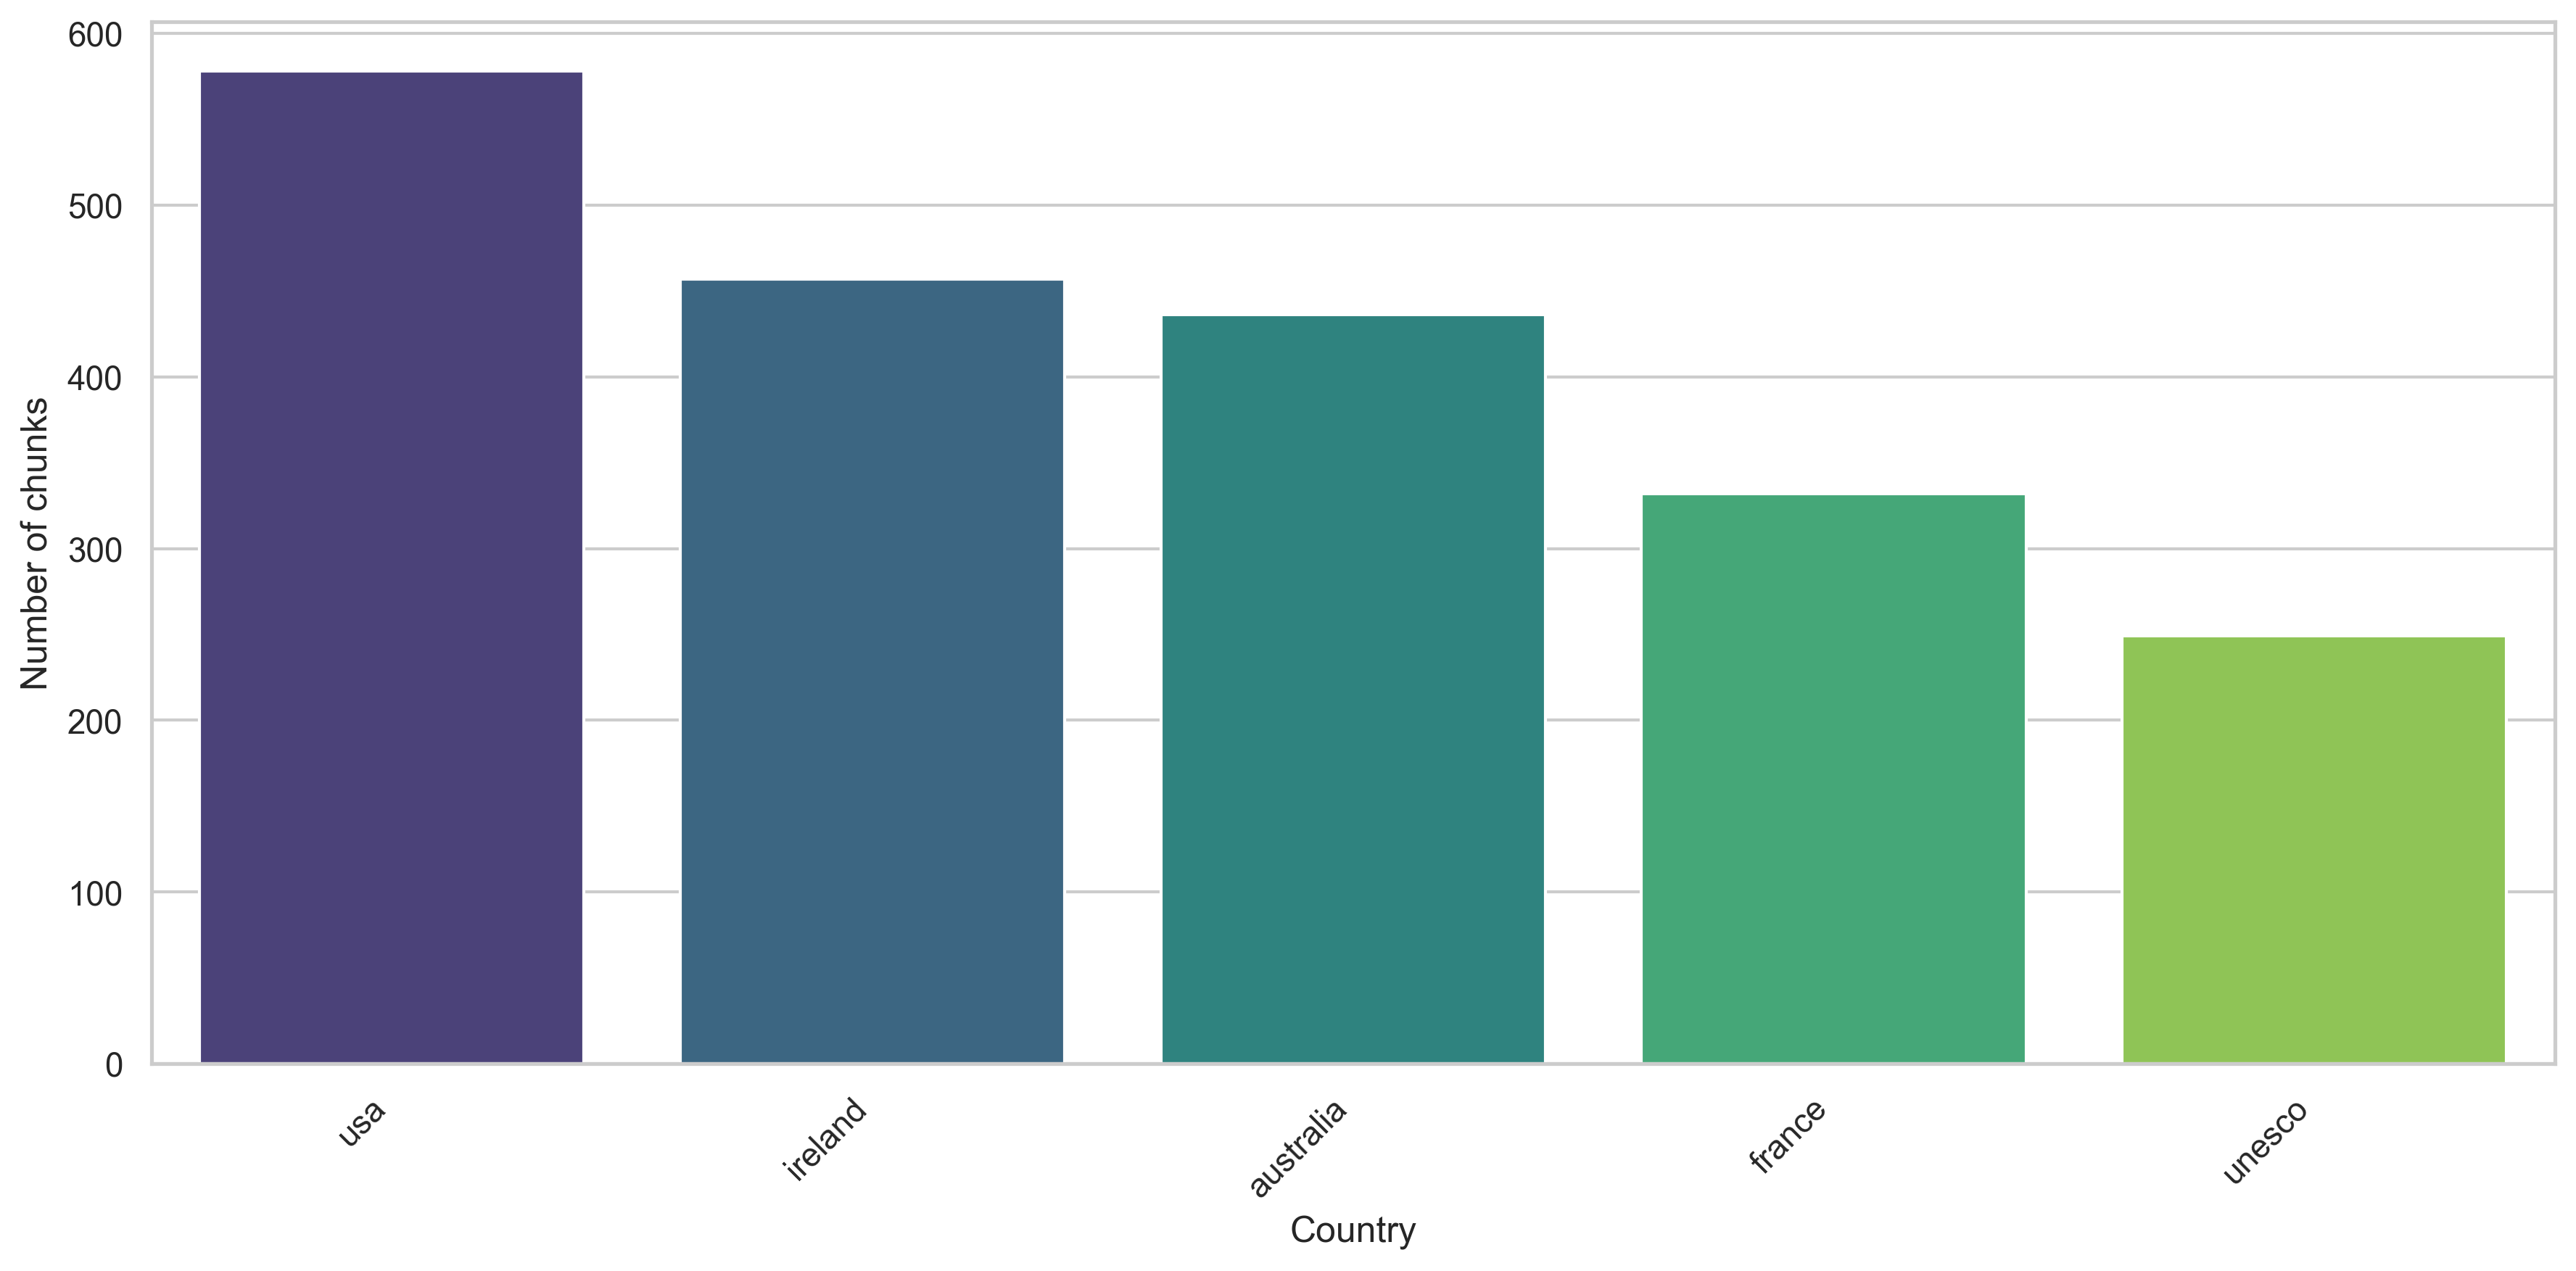
\includegraphics[width=\linewidth]{doc_count_per_country.png}
    \caption{Policy chunks by source group.}
    \label{fig:impl-country-chunks}
\end{subfigure}

\vspace{0.5em}

\begin{subfigure}[t]{0.49\textwidth}
    \centering
    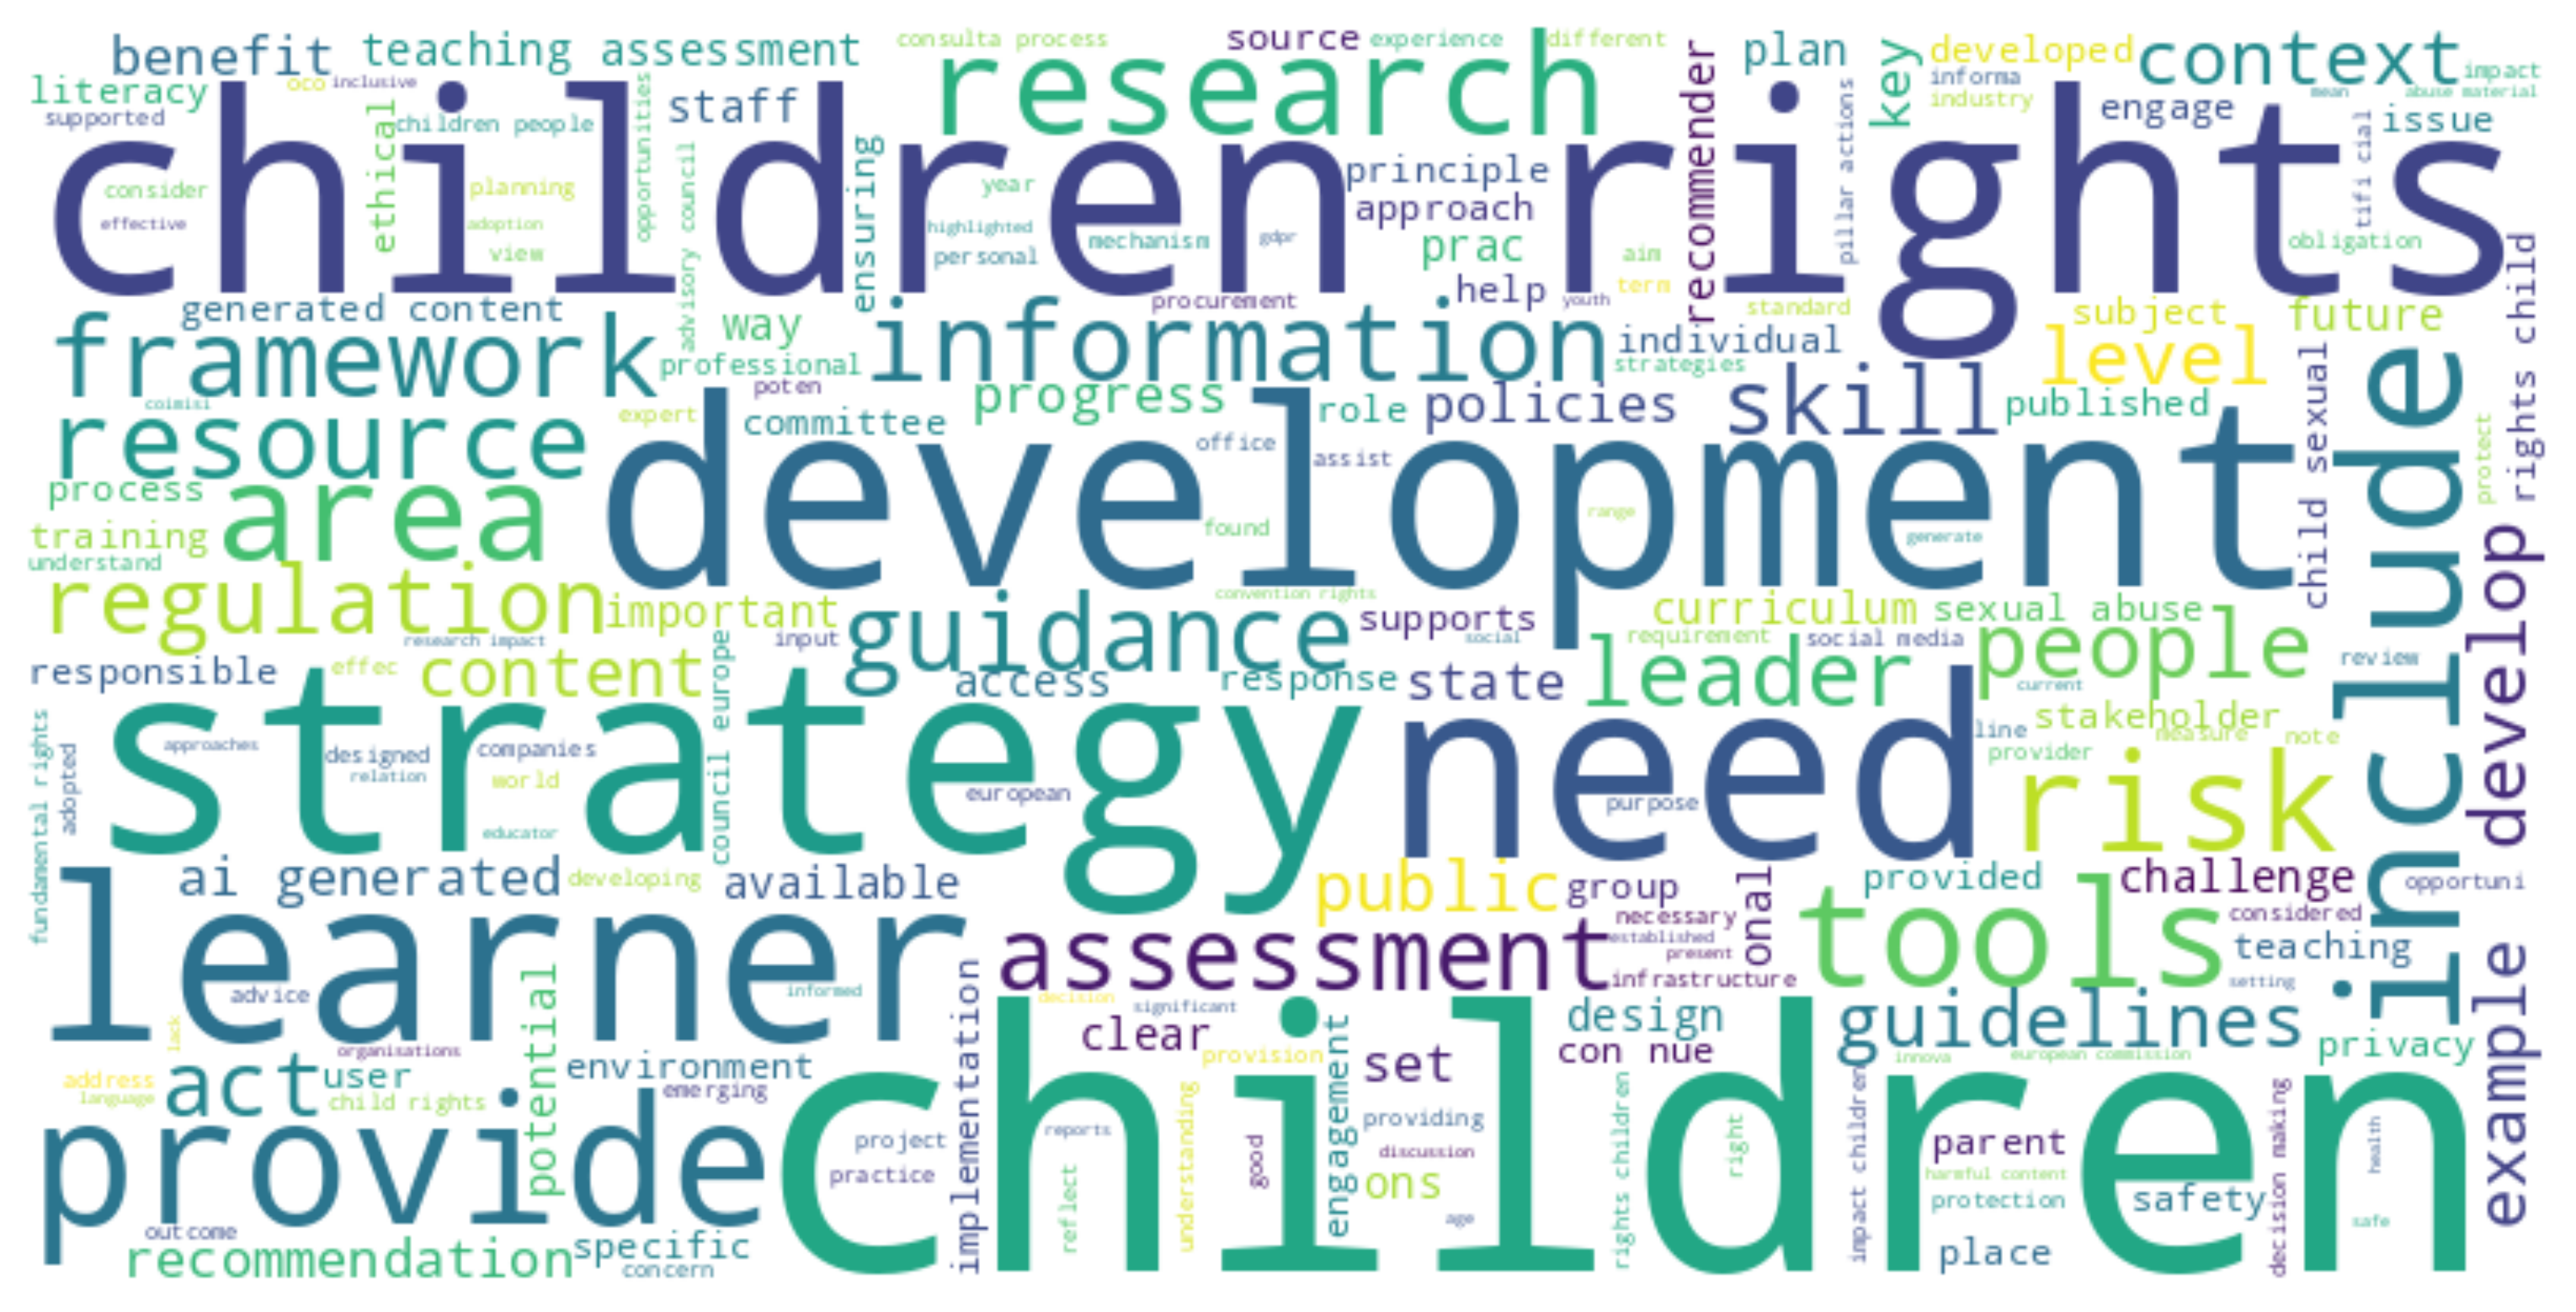
\includegraphics[width=\linewidth]{wordcloud_ireland.png}
    \caption{Irish policy corpus.}
    \label{fig:impl-wordcloud-ireland}
\end{subfigure}
\hfill
\begin{subfigure}[t]{0.49\textwidth}
    \centering
    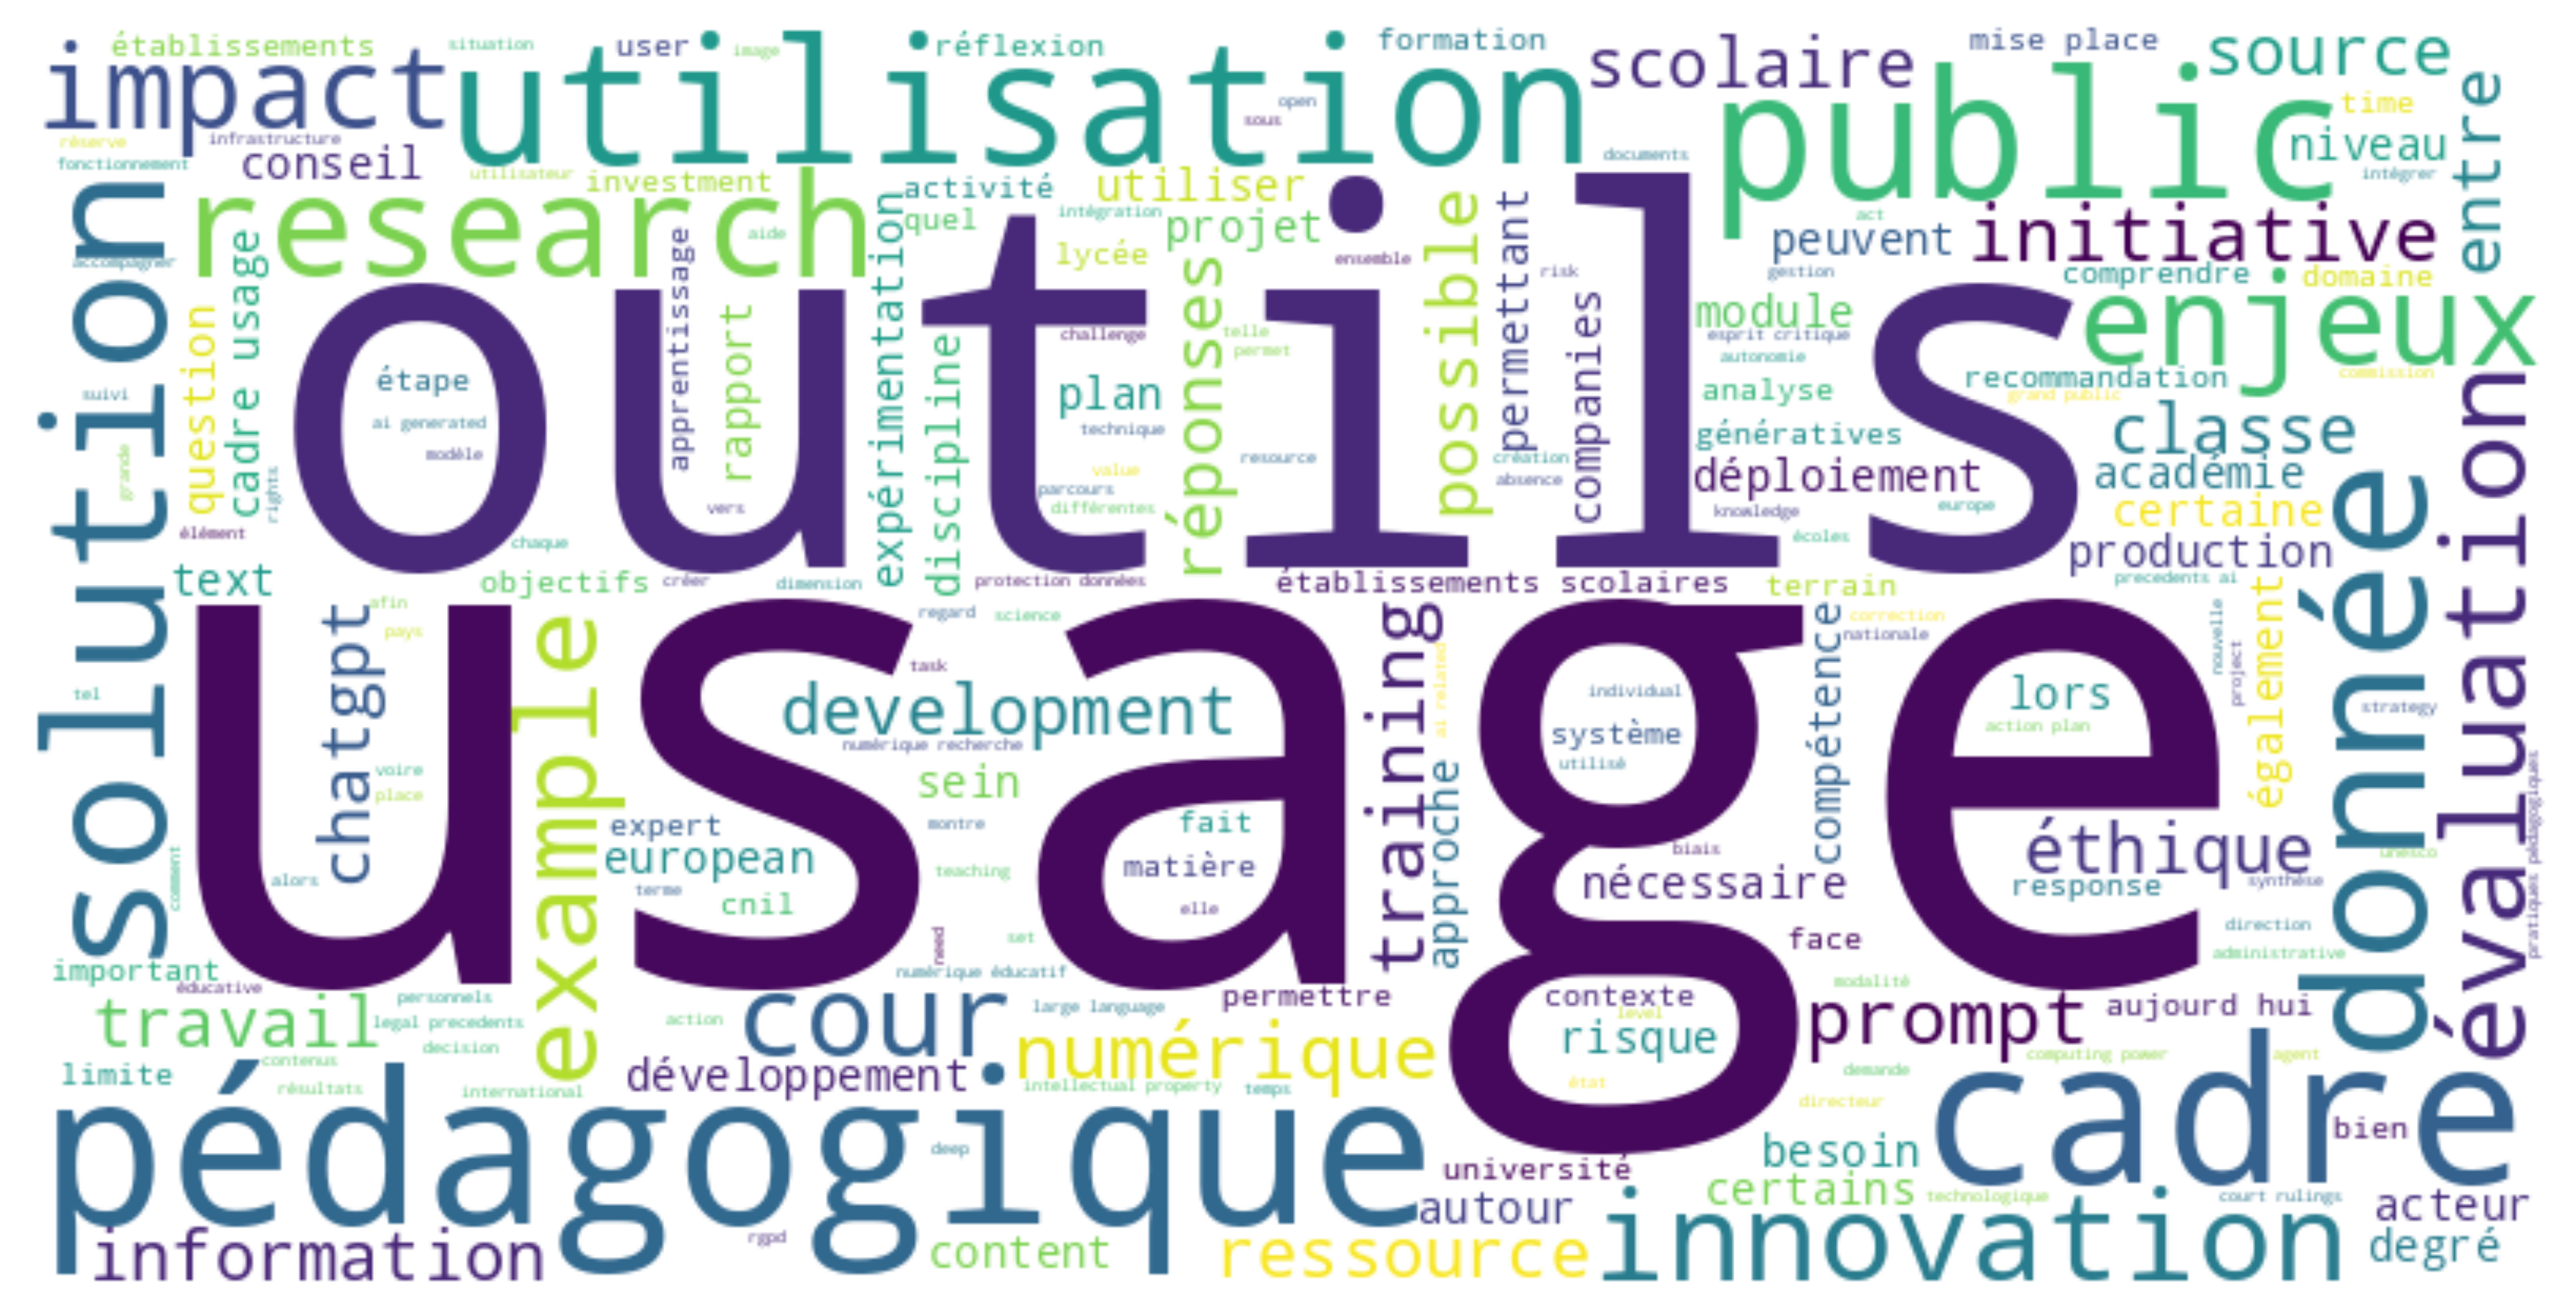
\includegraphics[width=\linewidth]{wordcloud_france.png}
    \caption{French policy corpus.}
    \label{fig:impl-wordcloud-france}
\end{subfigure}

\caption{Exploratory overview of source representation and recurrent vocabulary in
the policy corpus, including the combined collection and the Irish and French
subsets.}
\label{fig:impl-policy-exploration}
\end{figure}

\subsection{Exploratory Corpus Analysis}
\label{subsec:impl-corpus-exploration}

Before model fitting, exploratory analysis examined source representation, recurrent
vocabulary, and extraction artefacts. The policy exploration covered 2,052 chunks
from the United States, Ireland, Australia, France, and two UNESCO global documents
discussed in Chapter~\ref{chap:litrev} by \cite{miao2024aiteachers} and
\cite{miao2024aistudents}. As shown in
Figure~\ref{fig:impl-policy-exploration}, the United States contributed the largest
number of chunks, followed by Ireland and Australia, while France and the UNESCO
documents contributed smaller collections. The global policy word cloud contained
references to needs, tools, research, information, guidance, development, learning,
and resources.

Country-level word clouds were generated for the Irish and French policy collections.
The Irish corpus contained frequent references to children, rights, development,
learning, guidance, strategy, and resources. {\color{blue}These terms reflect
educational support, governance, and learner protection.}
The French corpus included both French and English vocabulary, with terms related
to usage, tools, pedagogical practice, evaluation, research, innovation, and public
institutions. {\color{blue}This indicates a focus on implementation, institutional
coordination, and pedagogical AI use.}

\begin{figure}[ht]
\centering

\begin{subfigure}[t]{0.49\textwidth}
    \centering
    
\includegraphics[width=\linewidth]{wordcloud_europe_sentiment.png}
    \caption{Europe-wide original sentiment word cloud.}
    \label{fig:impl-sentiment-europe-wordcloud}
\end{subfigure}
\hfill
\begin{subfigure}[t]{0.49\textwidth}
    \centering
    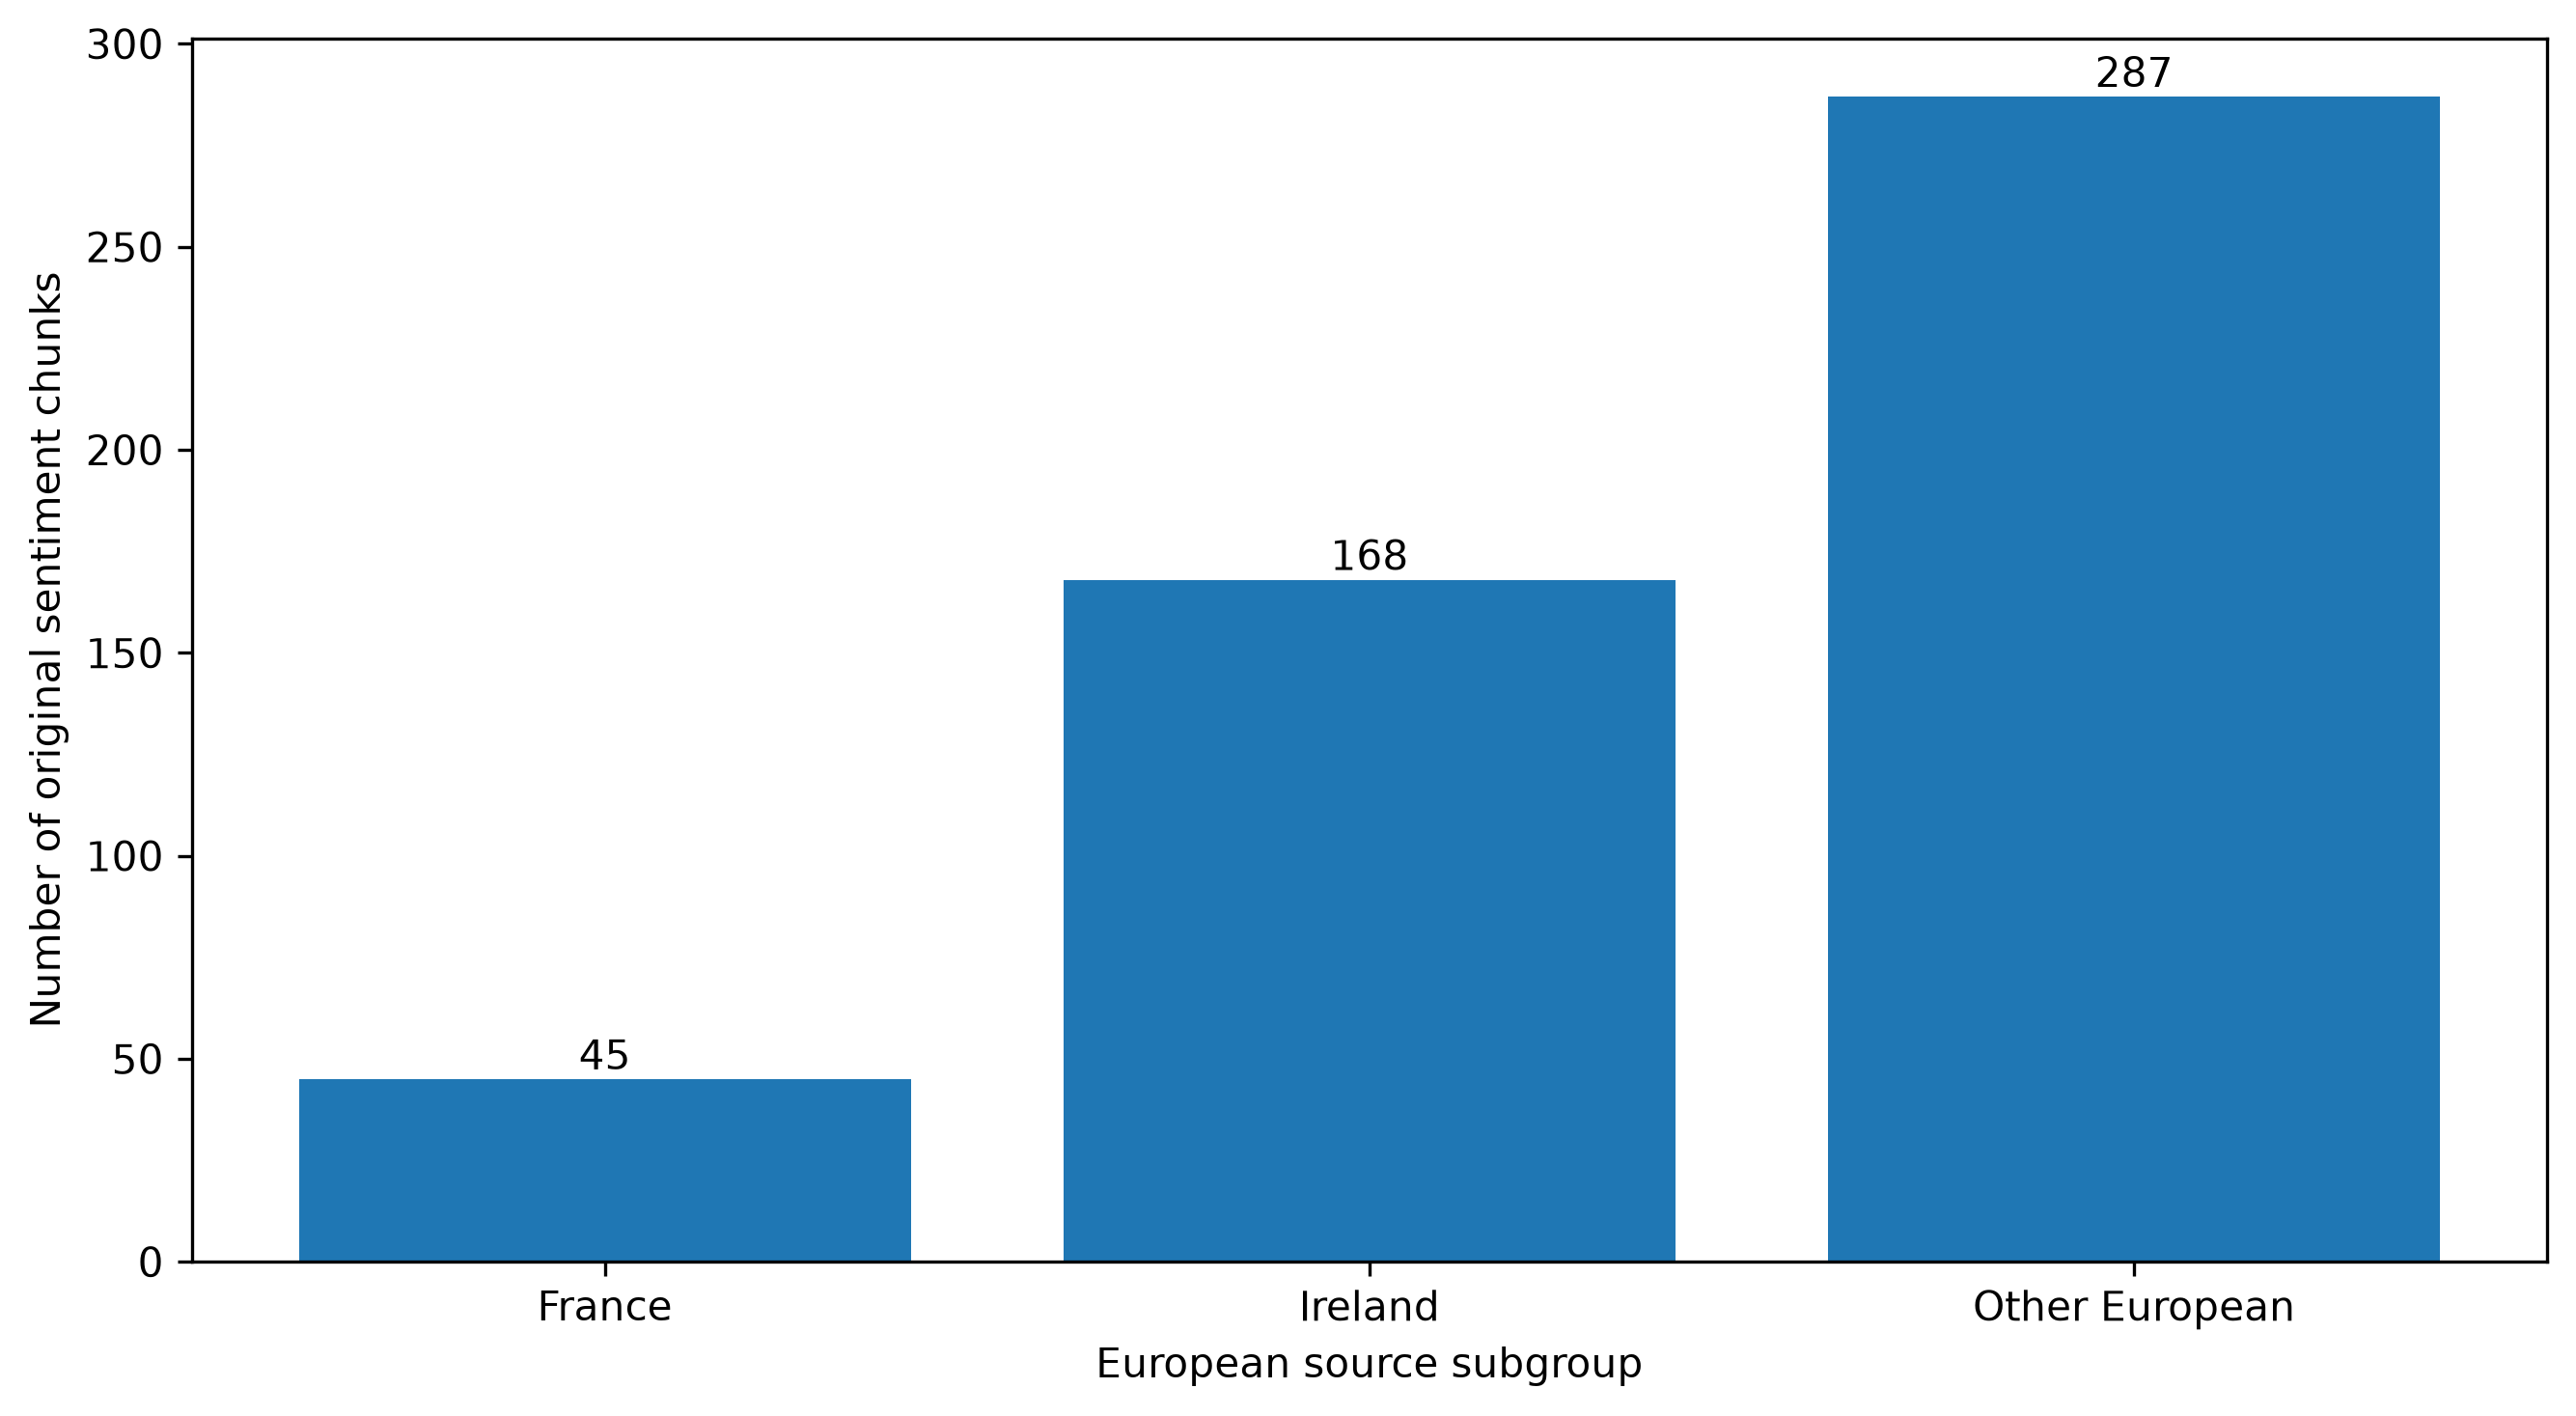
\includegraphics[width=\linewidth]{chunk_count_by_scope_sentiment.png}
    \caption{Chunks by European source subgroup.}
    \label{fig:impl-sentiment-scope-chunks}
\end{subfigure}

\vspace{0.5em}

\begin{subfigure}[t]{0.49\textwidth}
    \centering
    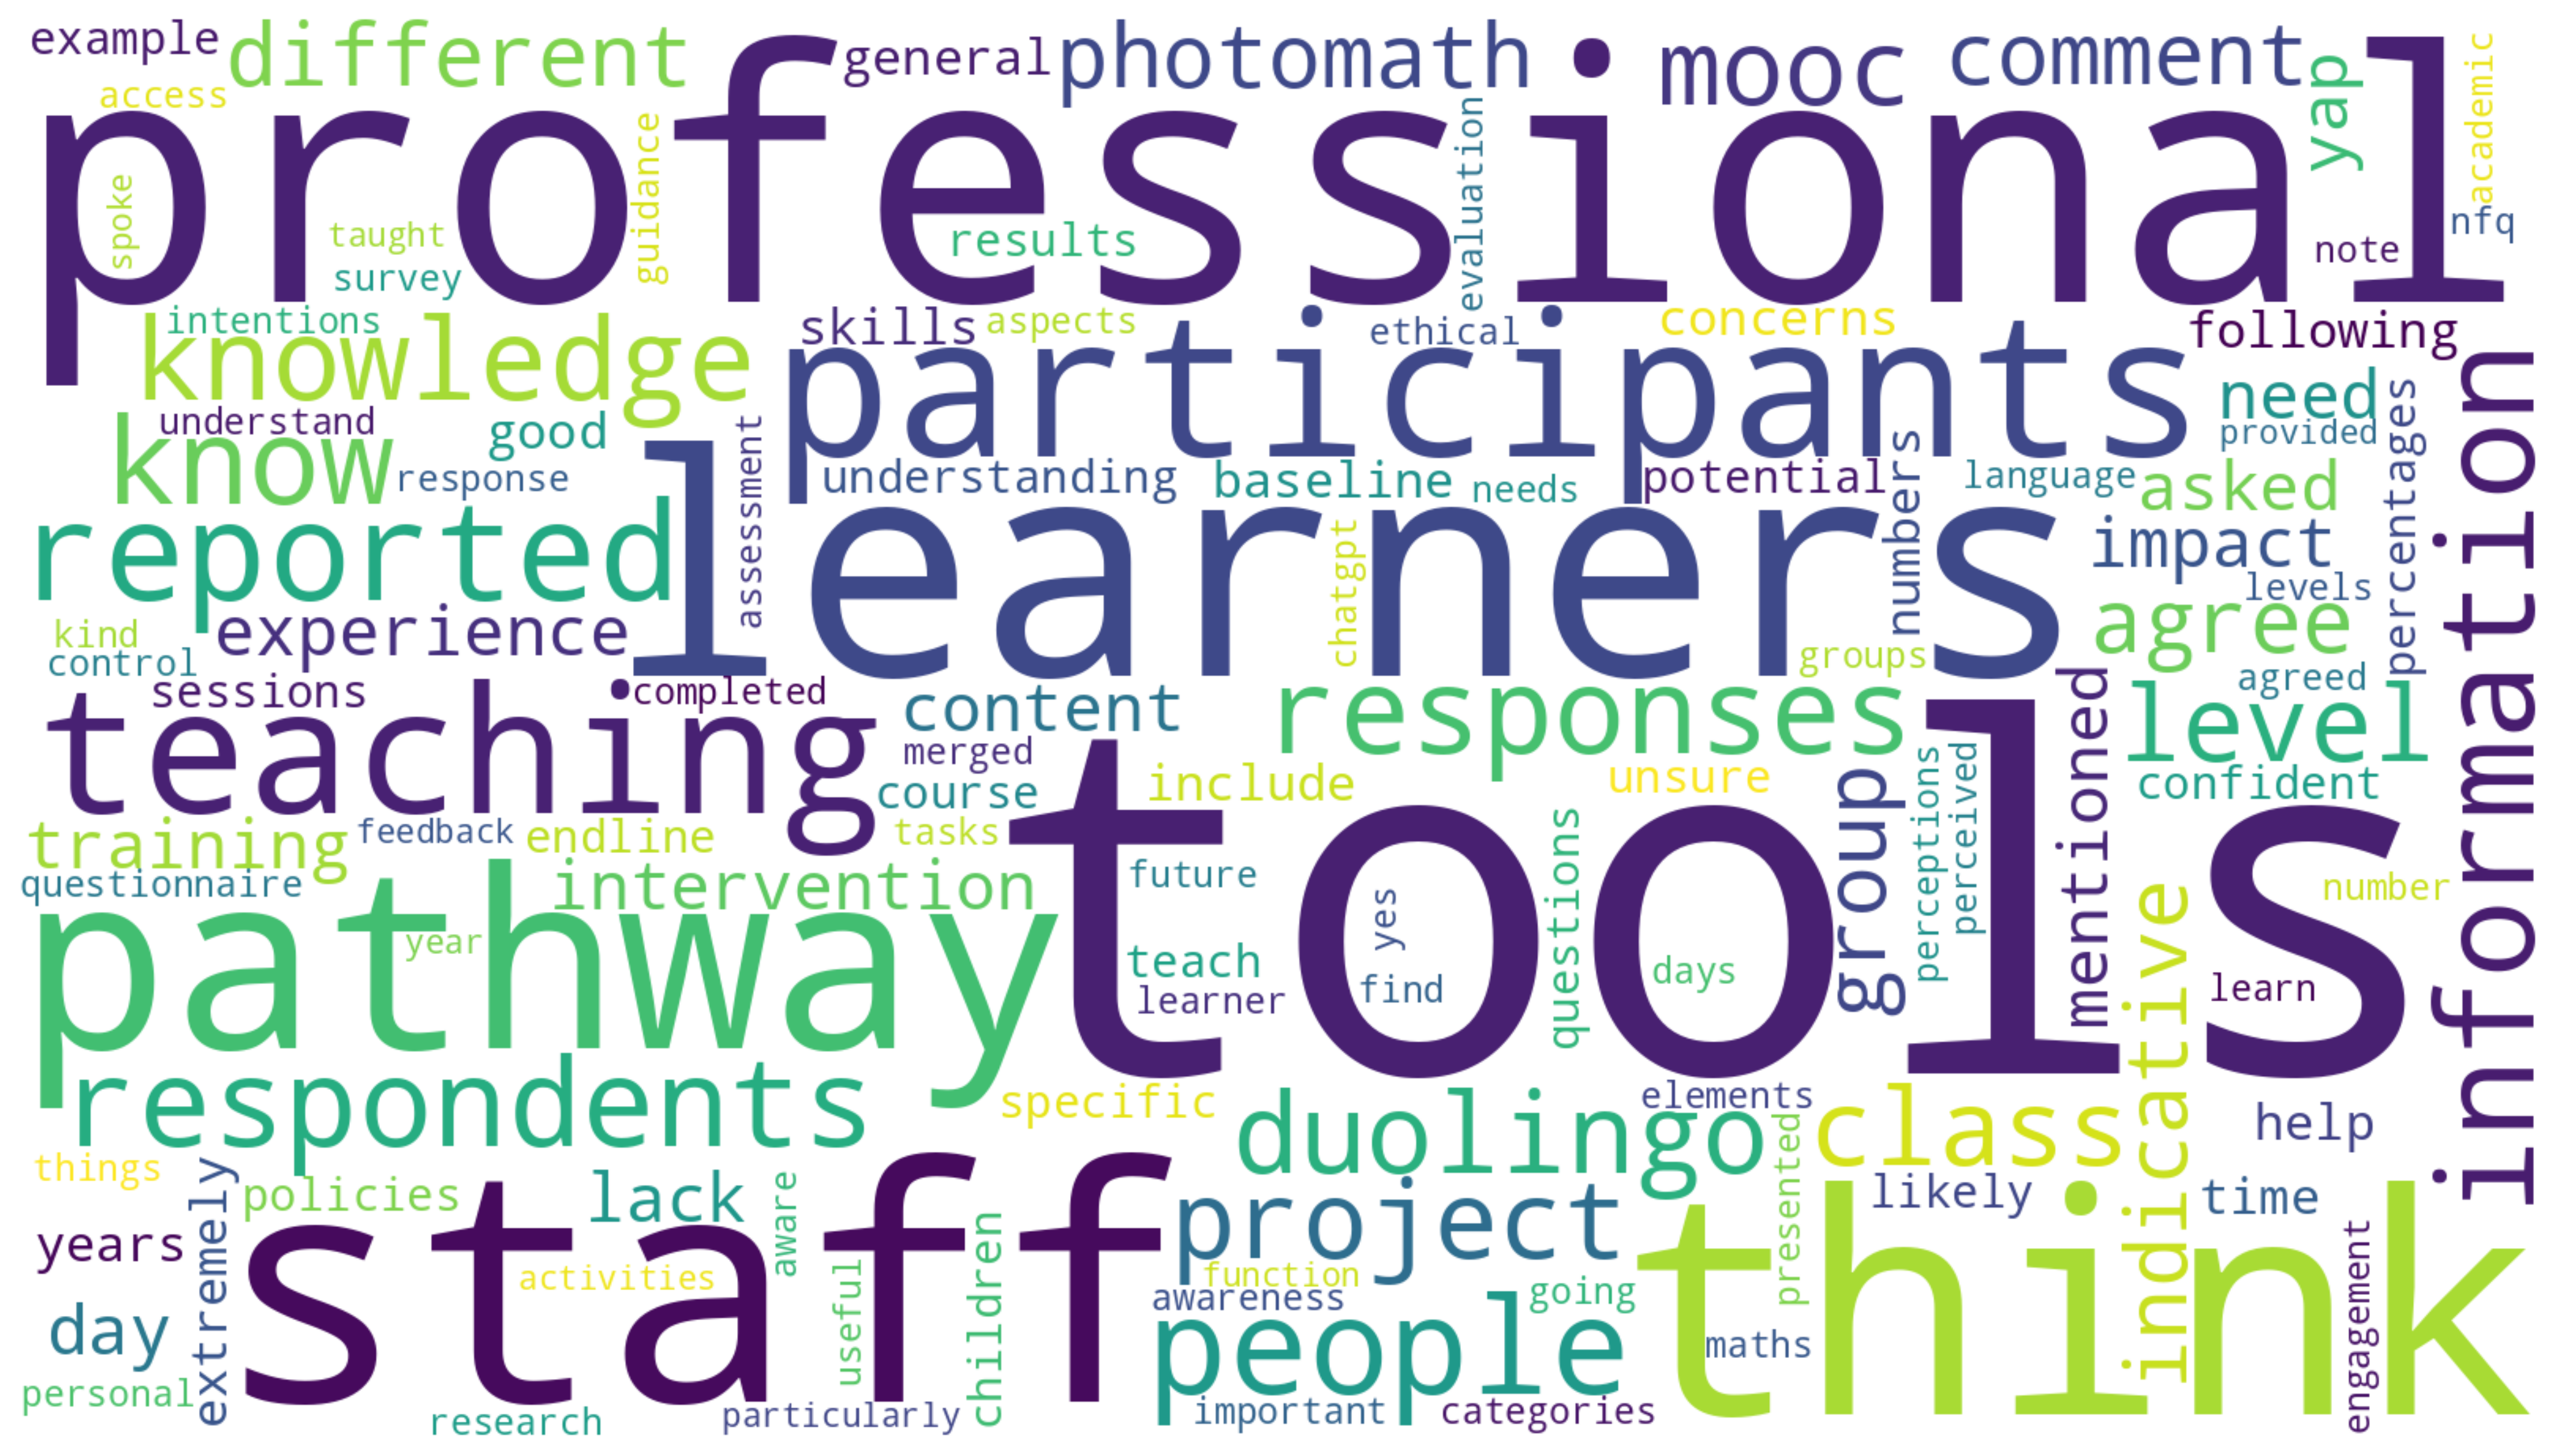
\includegraphics[width=\linewidth]{wordcloud_ireland_sentiment.png}
    \caption{Irish sentiment corpus.}
    \label{fig:impl-sentiment-wordcloud-ireland}
\end{subfigure}
\hfill
\begin{subfigure}[t]{0.49\textwidth}
    \centering
    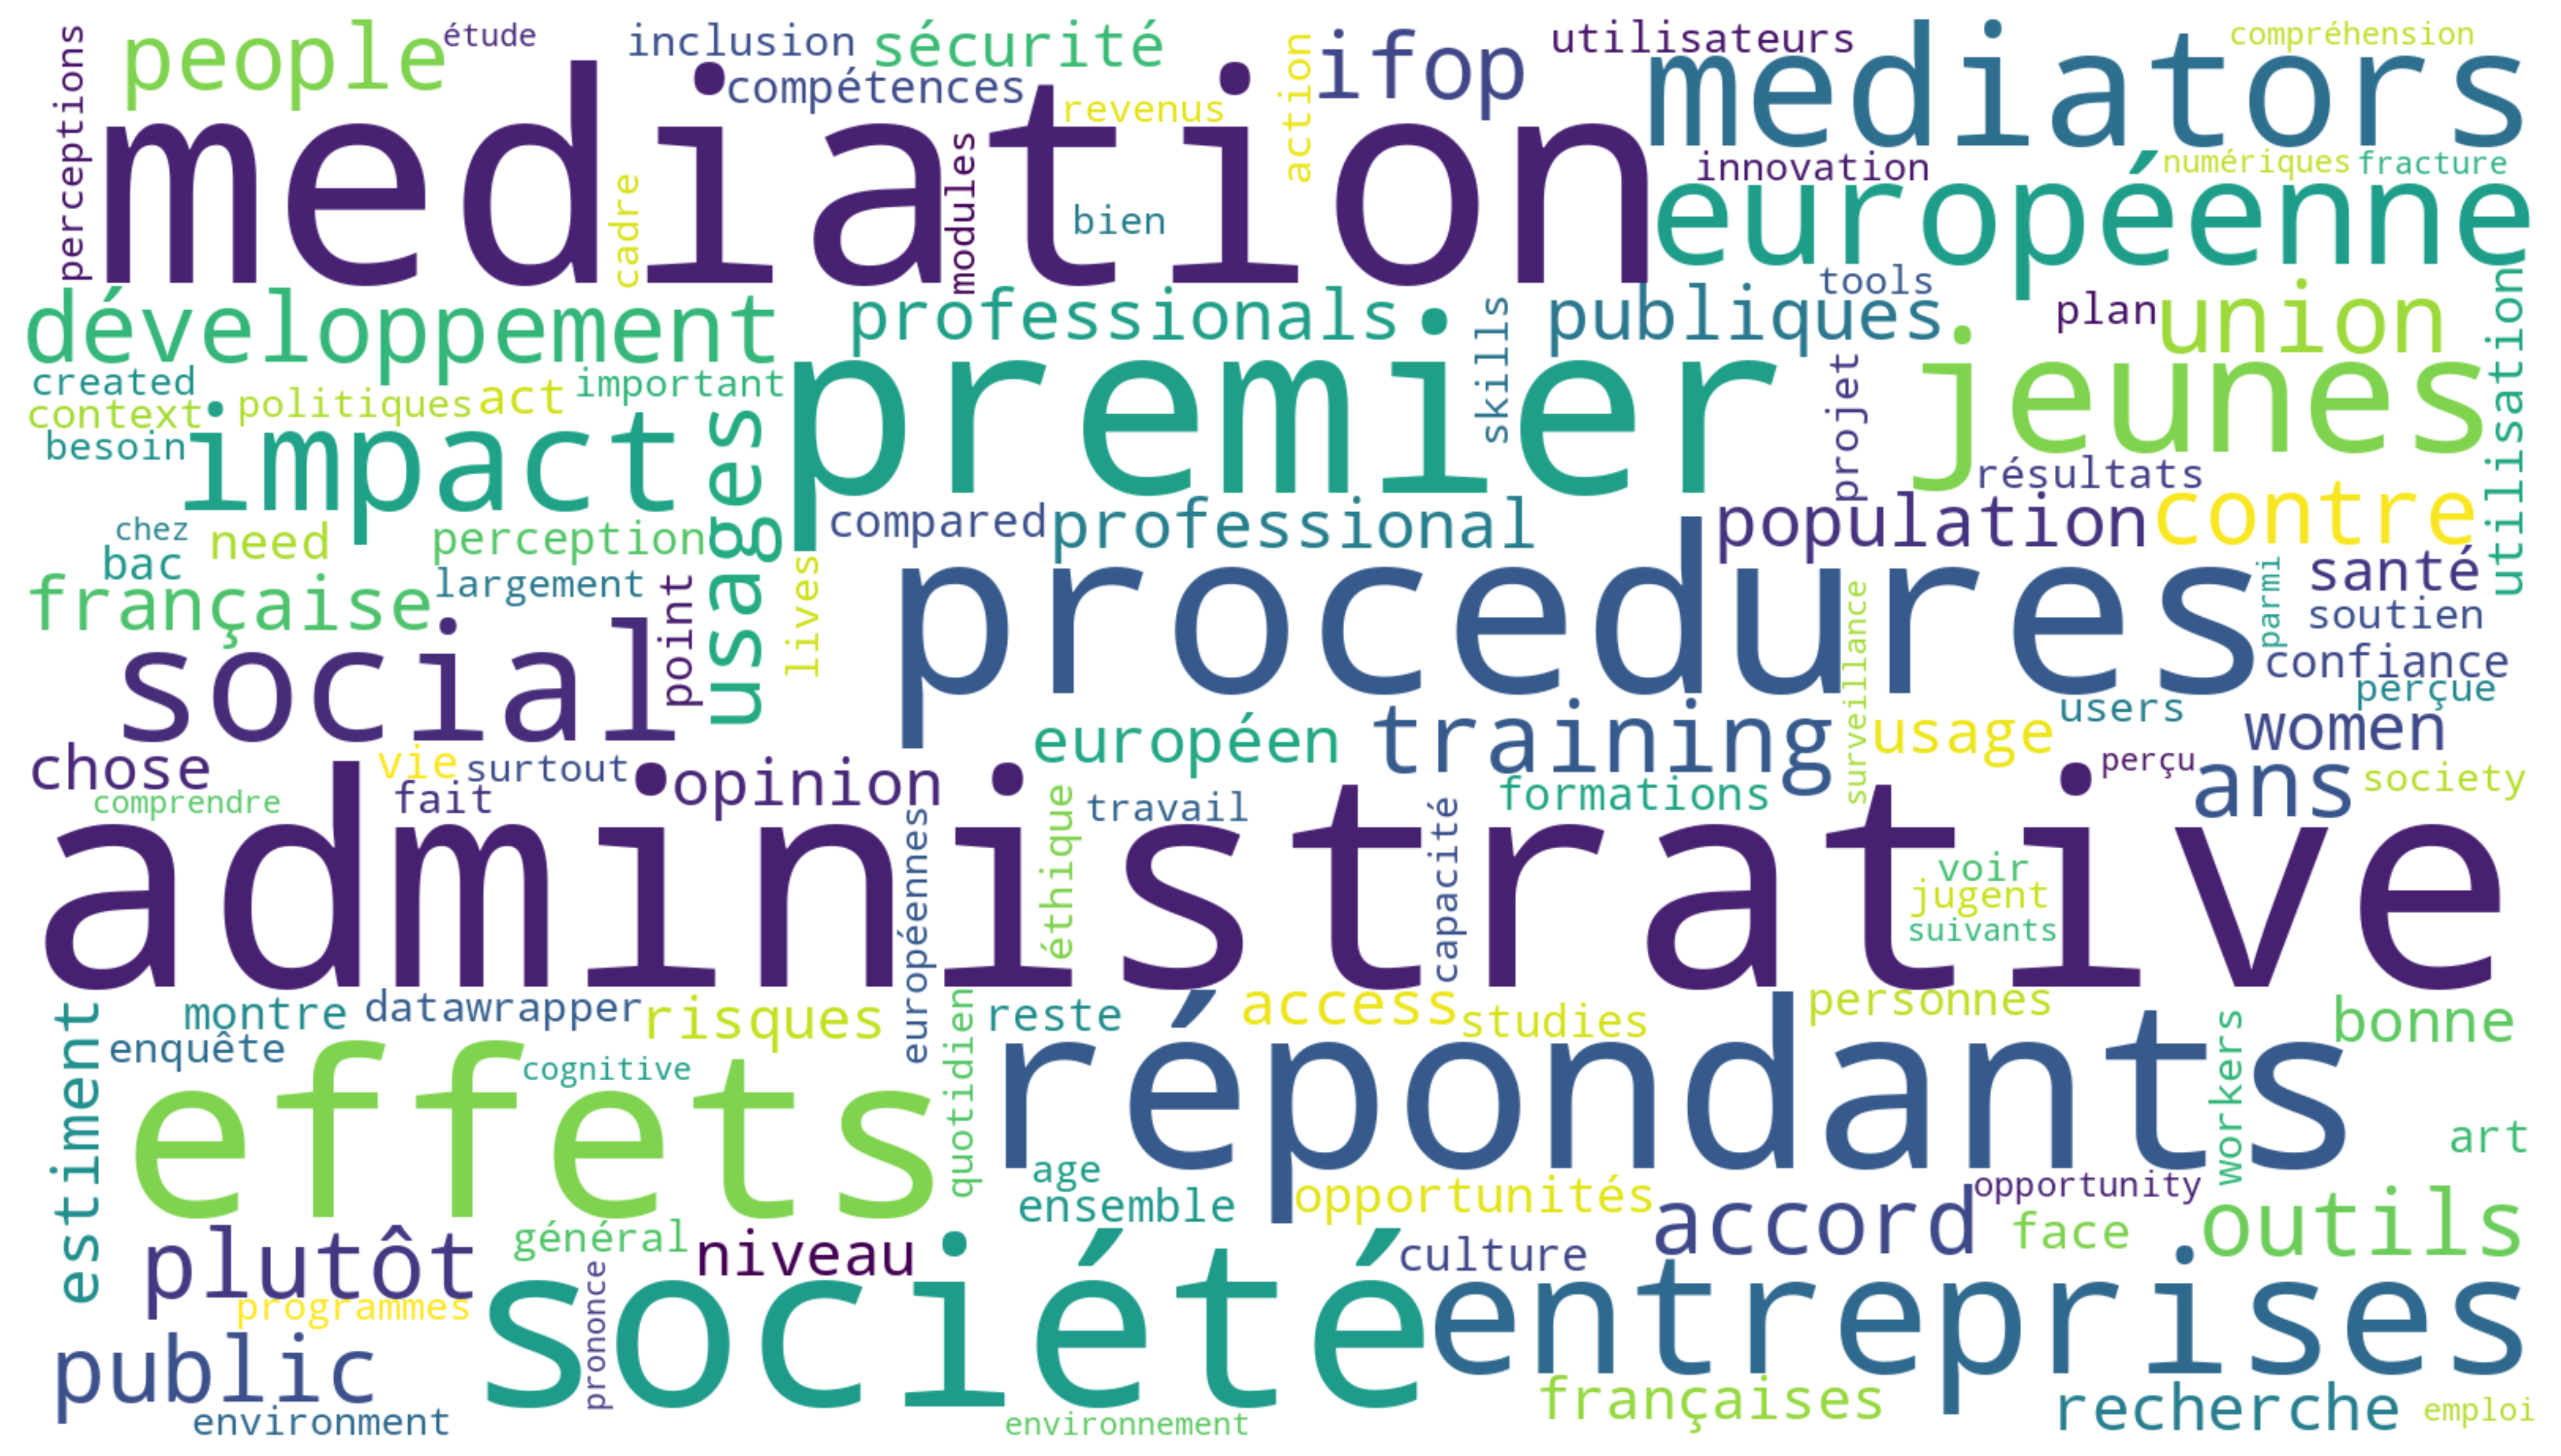
\includegraphics[width=\linewidth]{wordcloud_france_sentiment.png}
    \caption{French sentiment corpus.}
    \label{fig:impl-sentiment-wordcloud-france}
\end{subfigure}

\caption{Source representation and recurrent vocabulary in the European sentiment
corpus and its Irish and French subsets.}
\label{fig:impl-sentiment-exploration}
\end{figure}



The sentiment corpus was processed using the policy cleaning rules and stop-word
vocabulary. French and English variants of positive and negative were removed as
sentiment labels rather than substantive terms.
Figure~\ref{fig:impl-sentiment-exploration} shows the Europe-wide word cloud for the
corpus, whose reports concerned European contexts.

Because the sentiment \texttt{country} field was empty, source groups were assigned
from filenames, source paths, and document identifiers. French and Irish
indicators determined country assignment, while remaining reports were assigned
to \textit{Other European}. Manual overrides covered ambiguous source names.
Figure~\ref{fig:impl-sentiment-exploration} shows that the exploration retained
500 original-report chunks: 45 from France, 168 from Ireland, and 287 from
Other European sources. {\color{blue}The exploratory grouping compared
source balance and recurring vocabulary across the French, Irish, and
European subsets, while retaining provenance for interpretation and avoiding
claims of national representativeness.} In corpus-level analyses, the European
sentiment corpus provided a shared contextual baseline for France and Ireland,
reflecting limited national evidence and broadly convergent sentiment patterns
across European sources.

The word clouds in Figure~\ref{fig:impl-sentiment-exploration} show frequent
Europe-wide references to people, tools, teaching, practice, development, skills,
rights, ethics, training, impact, privacy, risk, and access. The French subset
included terms related to administration, respondents, mediation, enterprises,
institutions, employment, health, and security. The Irish subset included learners,
staff, teaching, training, educational pathways, participants, classroom activities,
evaluation, and reported outcomes.

The exploratory results must be interpreted cautiously because source frequencies
reflect unequal document availability rather than equal international weighting.
Vocabulary differences may also arise from document genre, with policy texts
emphasising guidance and resources, and sentiment reports focusing more on people,
practice, privacy, risk, and access. Figure~\ref{fig:impl-sentiment-exploration} was
therefore used descriptively rather than as evidence of policy effectiveness,
national opinion, or causal relationships.


\section{Topic-Modelling Pipelines and Thematic Analysis}
\label{sec:impl-topic-modelling}

Following corpus construction, the study applied topic modelling to compare the
thematic structures of the policy and sentiment corpora. This section presents the
LDA, BERTopic-style, and NMF pipelines defined in
Section~\ref{sec:method-topic-modelling}, including candidate models, retained topic
counts, labels, country-level distributions, and synthetic-sentiment robustness
checks. The analysis is included here because the thematic differences address the
research question and define the topic spaces used by the causal NLP methods.

\subsection{Shared Topic-Labelling and Robustness Procedures}
\label{subsec:impl-topic-labelling}

As defined in Subsections~\ref{subsec:method-bertopic} and
\ref{subsec:method-nmf}, BERTopic and NMF used
{\color{blue}the instruction-tuned SLM} \texttt{Qwen/Qwen2.5-1.5B-Instruct}, only after fitting. It generated labels from keywords and
representative chunks, which were reviewed before use. The SLM did not alter
assignments, shares, scores, or distributions.

\begin{verbatim}
Fitted BERTopic or NMF topics
  -> extract top keywords and representative chunks
  -> send these summaries to Qwen2.5-1.5B-Instruct
  -> generate a short topic phrase and prototype sentence
  -> attach the final label without changing topic assignments
\end{verbatim}


Synthetic sentiment remained separately labelled and was used only for sensitivity
and robustness checks. As discussed in
Subsection~\ref{subsec:method-synthetic-robustness}, it was not allowed to define the
empirical sentiment topic structure. LDA fitted separate models to the original and
synthetic sentiment corpora because its role was to provide an exploratory lexical
stress test. Independent fitting allowed the analysis to determine whether the
synthetic corpus produced a different optimal topic count, vocabulary structure, or
set of themes rather than forcing it into topics discovered from the original
reports. The comparison therefore examined changes in the discovered structures
rather than directly aligned topic shares.

BERTopic and NMF instead fitted their empirical sentiment models only on original
chunks and then assigned synthetic chunks to the retained topic spaces. Freezing the
original topics prevented synthetic material from changing the clusters, factors, or
topic definitions. It also enabled direct comparison of topic coverage and shares,
showing which empirical themes were over-represented, under-represented, or absent in
the synthetic corpus.

\begin{verbatim}
Original sentiment chunks
  -> fit the empirical topic model
  -> retain topics, assignments, and topic shares

Synthetic sentiment chunks
  -> apply the same preprocessing rules
  -> LDA: fit a separate model to compare discovered structures
  -> BERTopic/NMF: assign chunks to the fitted original topic space
  -> compare topic coverage and topic shares
  -> export sensitivity and robustness results
\end{verbatim}


\subsection{LDA Lexical Baseline}
\label{subsec:impl-lda}

LDA provided a lexical topic representation. As defined in
Subsection~\ref{subsec:method-lda}, cleaned chunks were converted into document--term
matrices. Candidate counts were assessed using coherence and diversity. Policy
models were fitted globally and by country; sentiment corpora separately.
{\color{blue}Gensim used \texttt{alpha="auto"} and \texttt{eta="auto"}, learning the
document--topic and topic--word priors from the corpus during fitting.} LDA served as
the baseline for later topic-modelling pipeline comparisons.


\begin{verbatim}
Policy or sentiment chunks
  -> select the corpus or country subset
  -> lowercase, tokenise, and remove stopwords
  -> lemmatise the retained tokens
  -> remove weak, short, or repeated chunks
  -> build a dictionary and document-term matrix
  -> fit candidate LDA topic models
  -> compare coherence and topic diversity
  -> retain and export the selected model
\end{verbatim}



\begin{figure}[!htbp]
\centering
\begin{subfigure}[t]{0.32\textwidth}
  \centering
  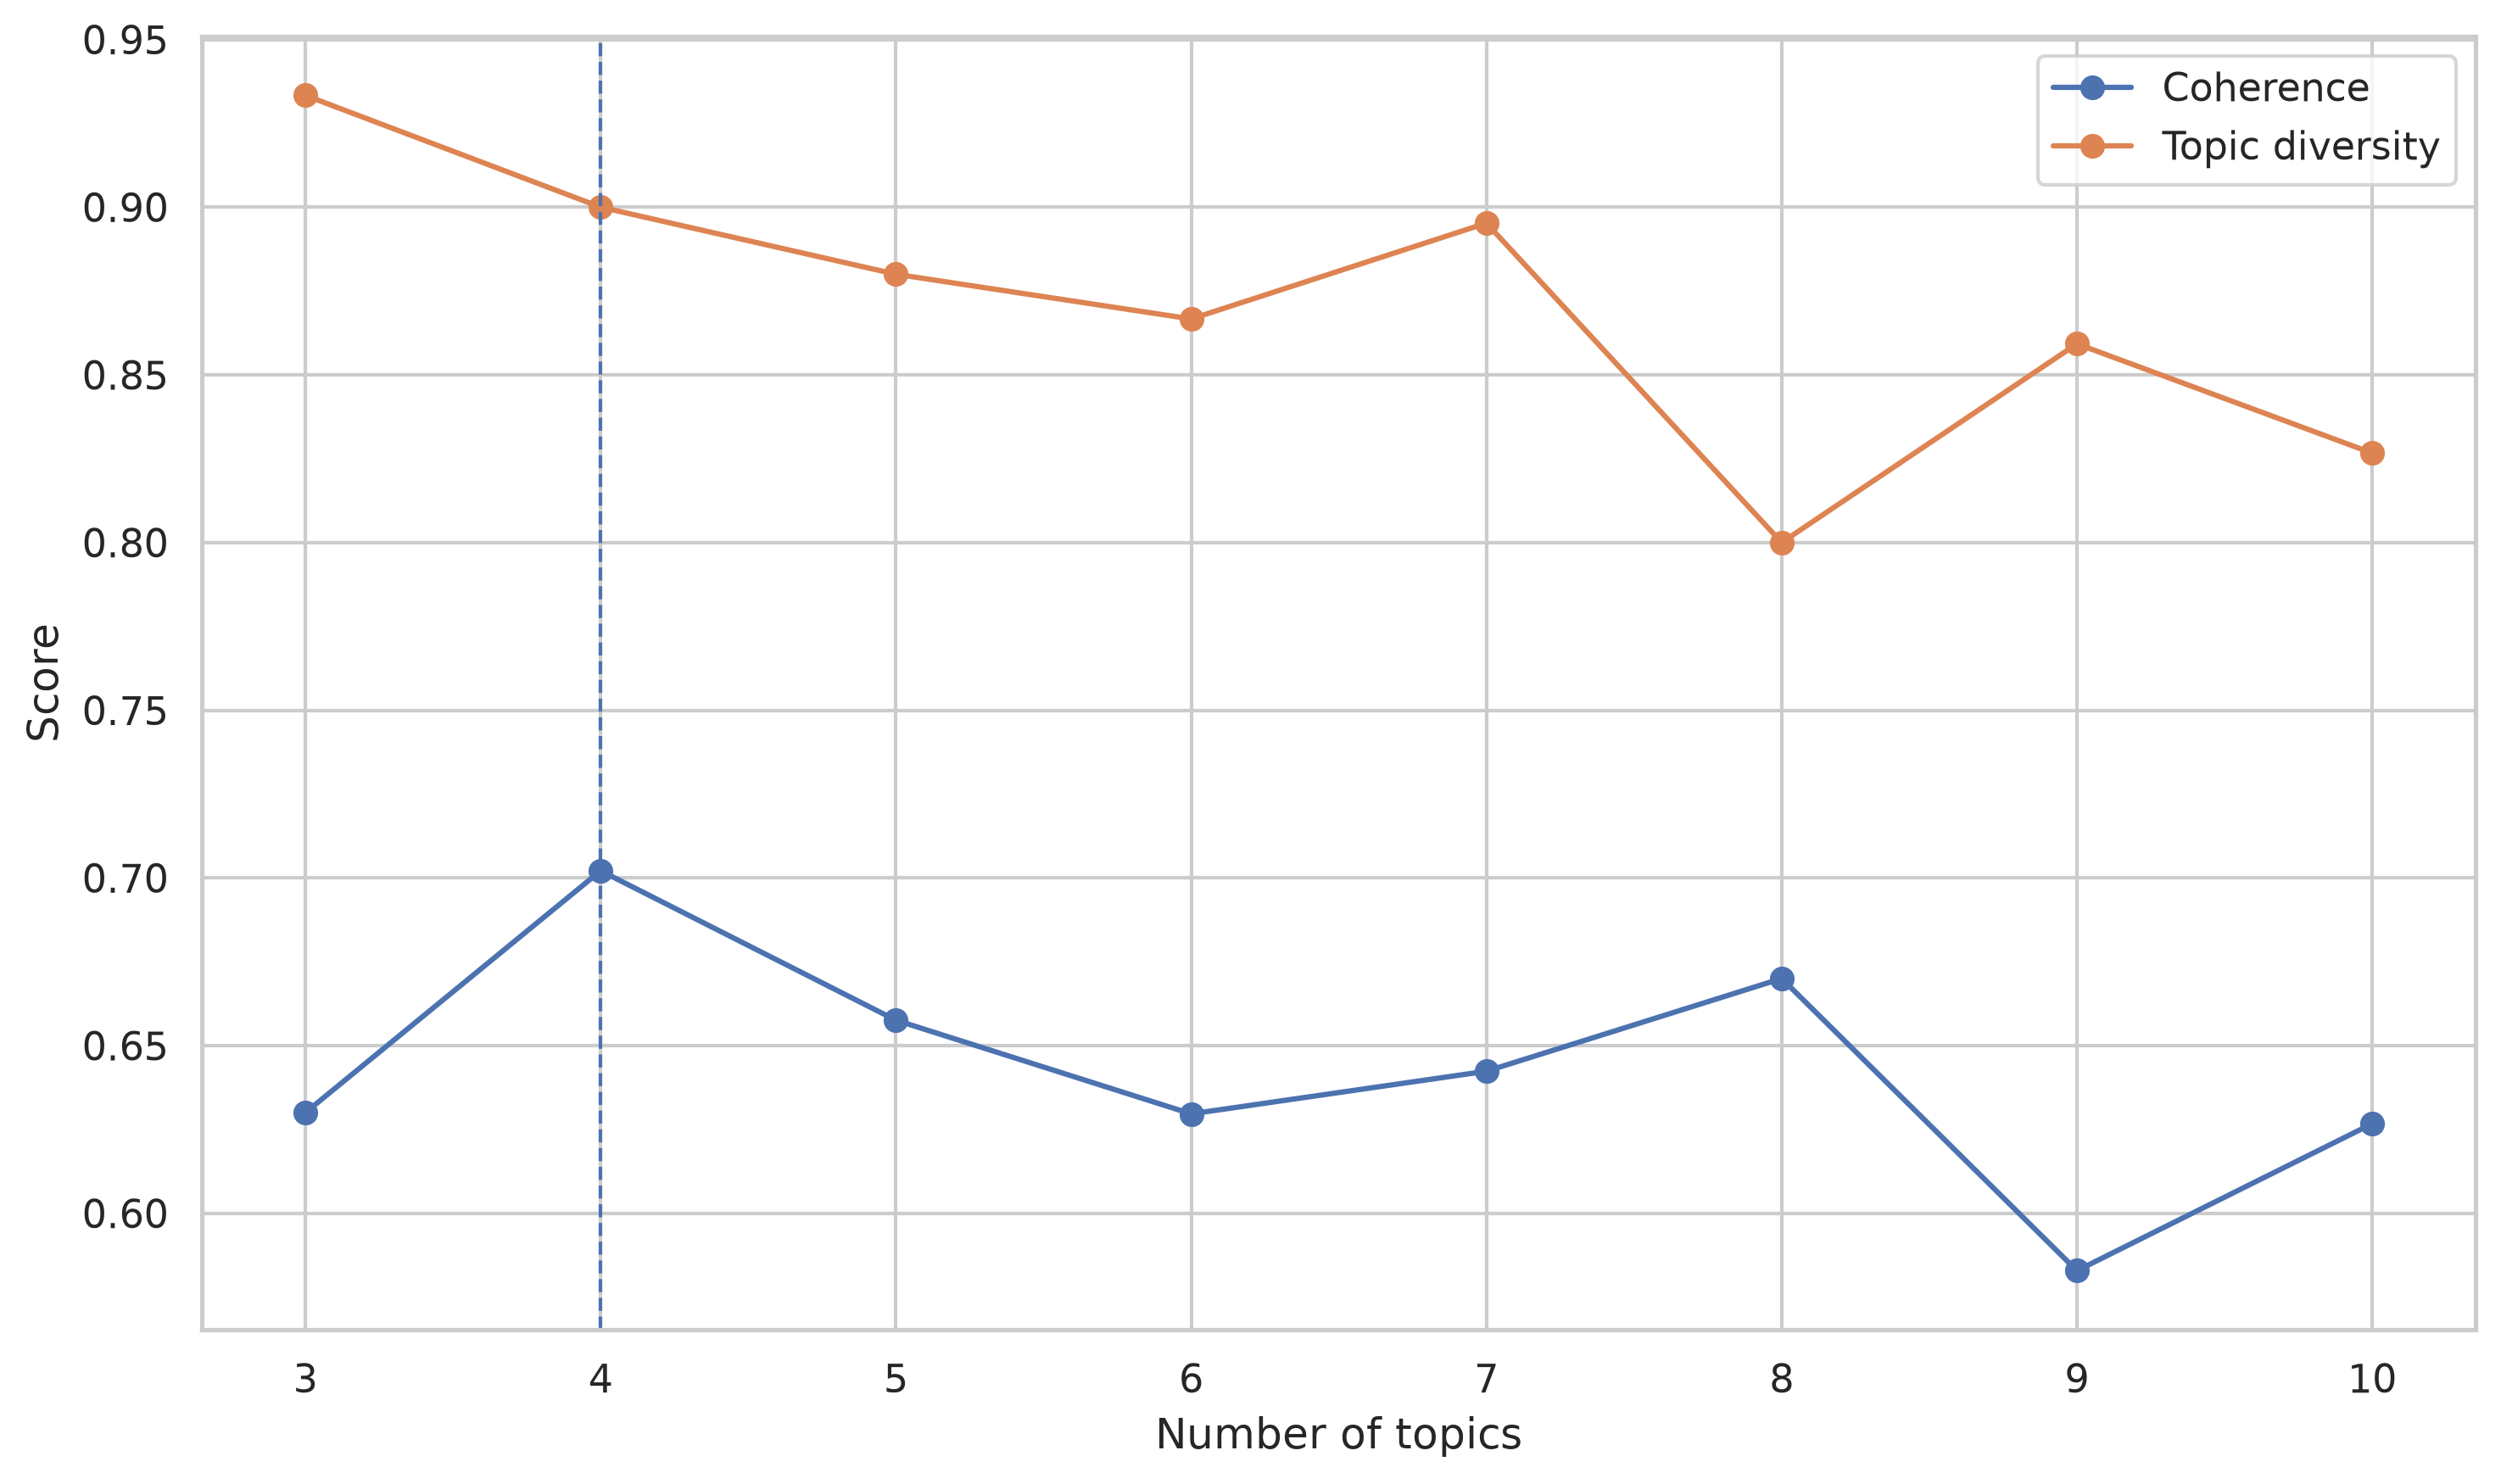
\includegraphics[width=\linewidth]{lda_policy_global_coherence_diversity.png}
  \caption{Policy search.}
  \label{fig:impl-lda-policy-search}
\end{subfigure}
\hfill
\begin{subfigure}[t]{0.32\textwidth}
  \centering
  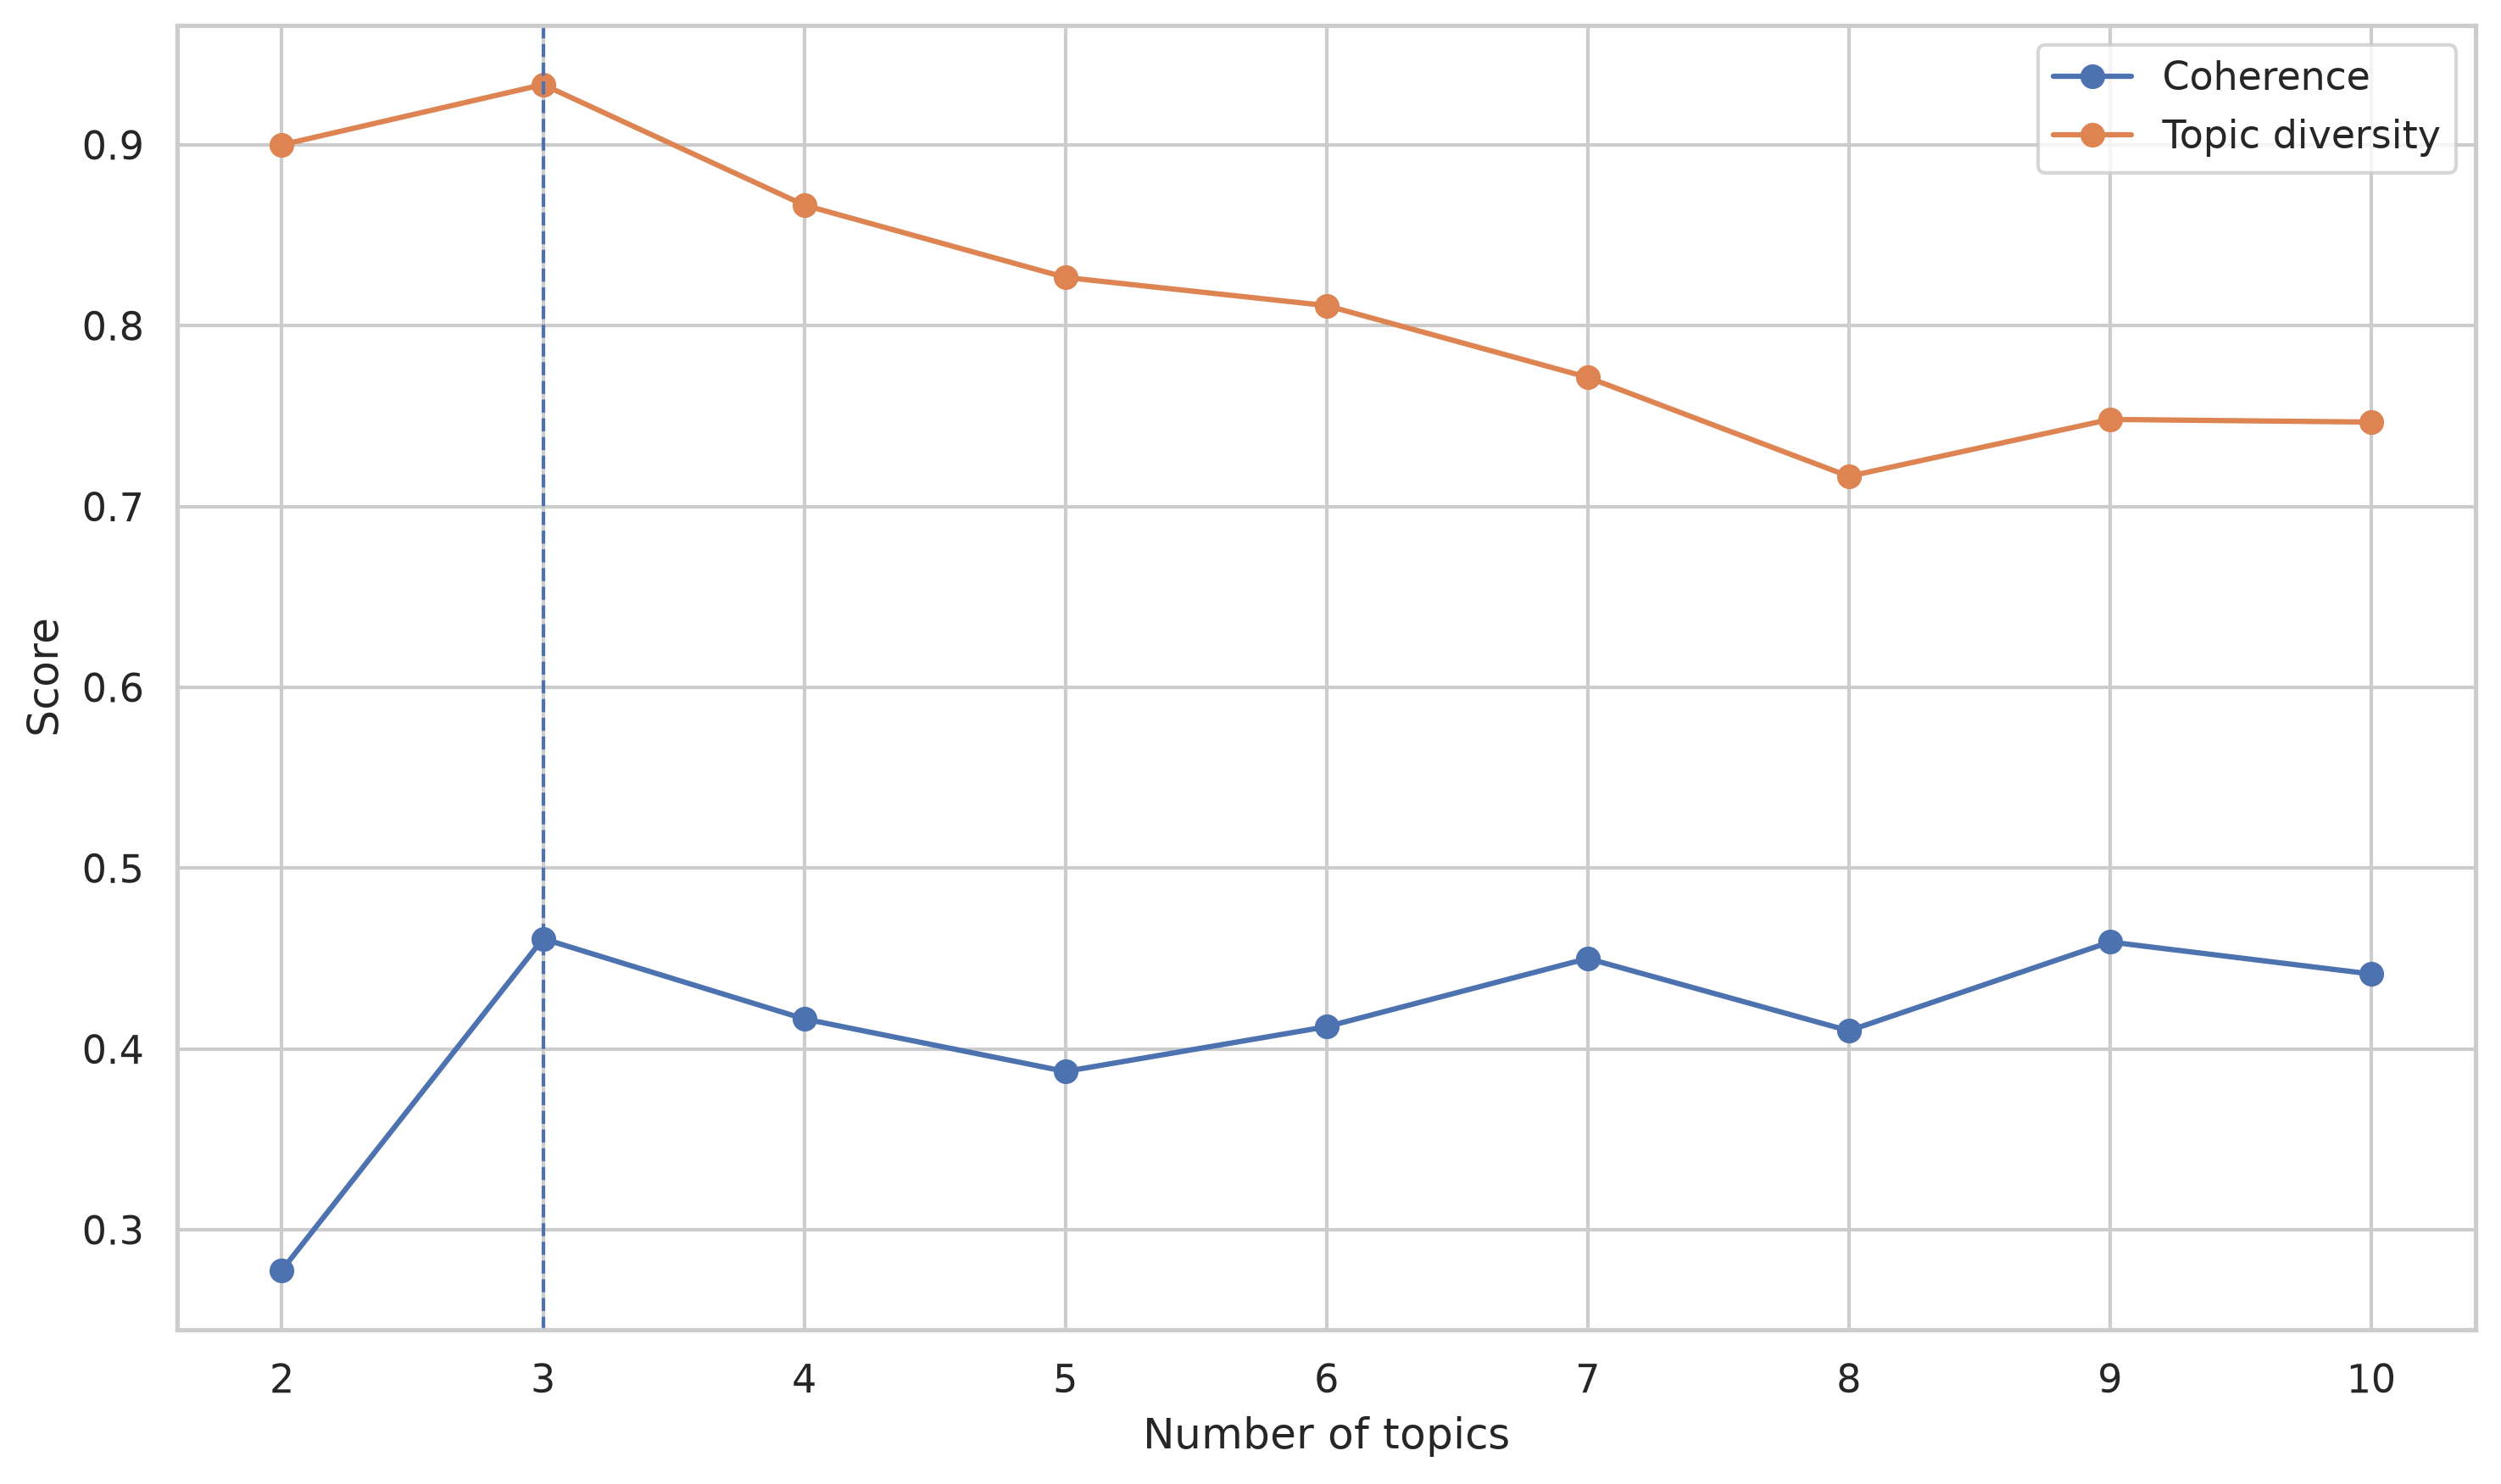
\includegraphics[width=\linewidth]{lda_sentiment_original_coherence_diversity.png}
  \caption{Original sentiment search.}
  \label{fig:impl-lda-original-search}
\end{subfigure}
\hfill
\begin{subfigure}[t]{0.32\textwidth}
  \centering
  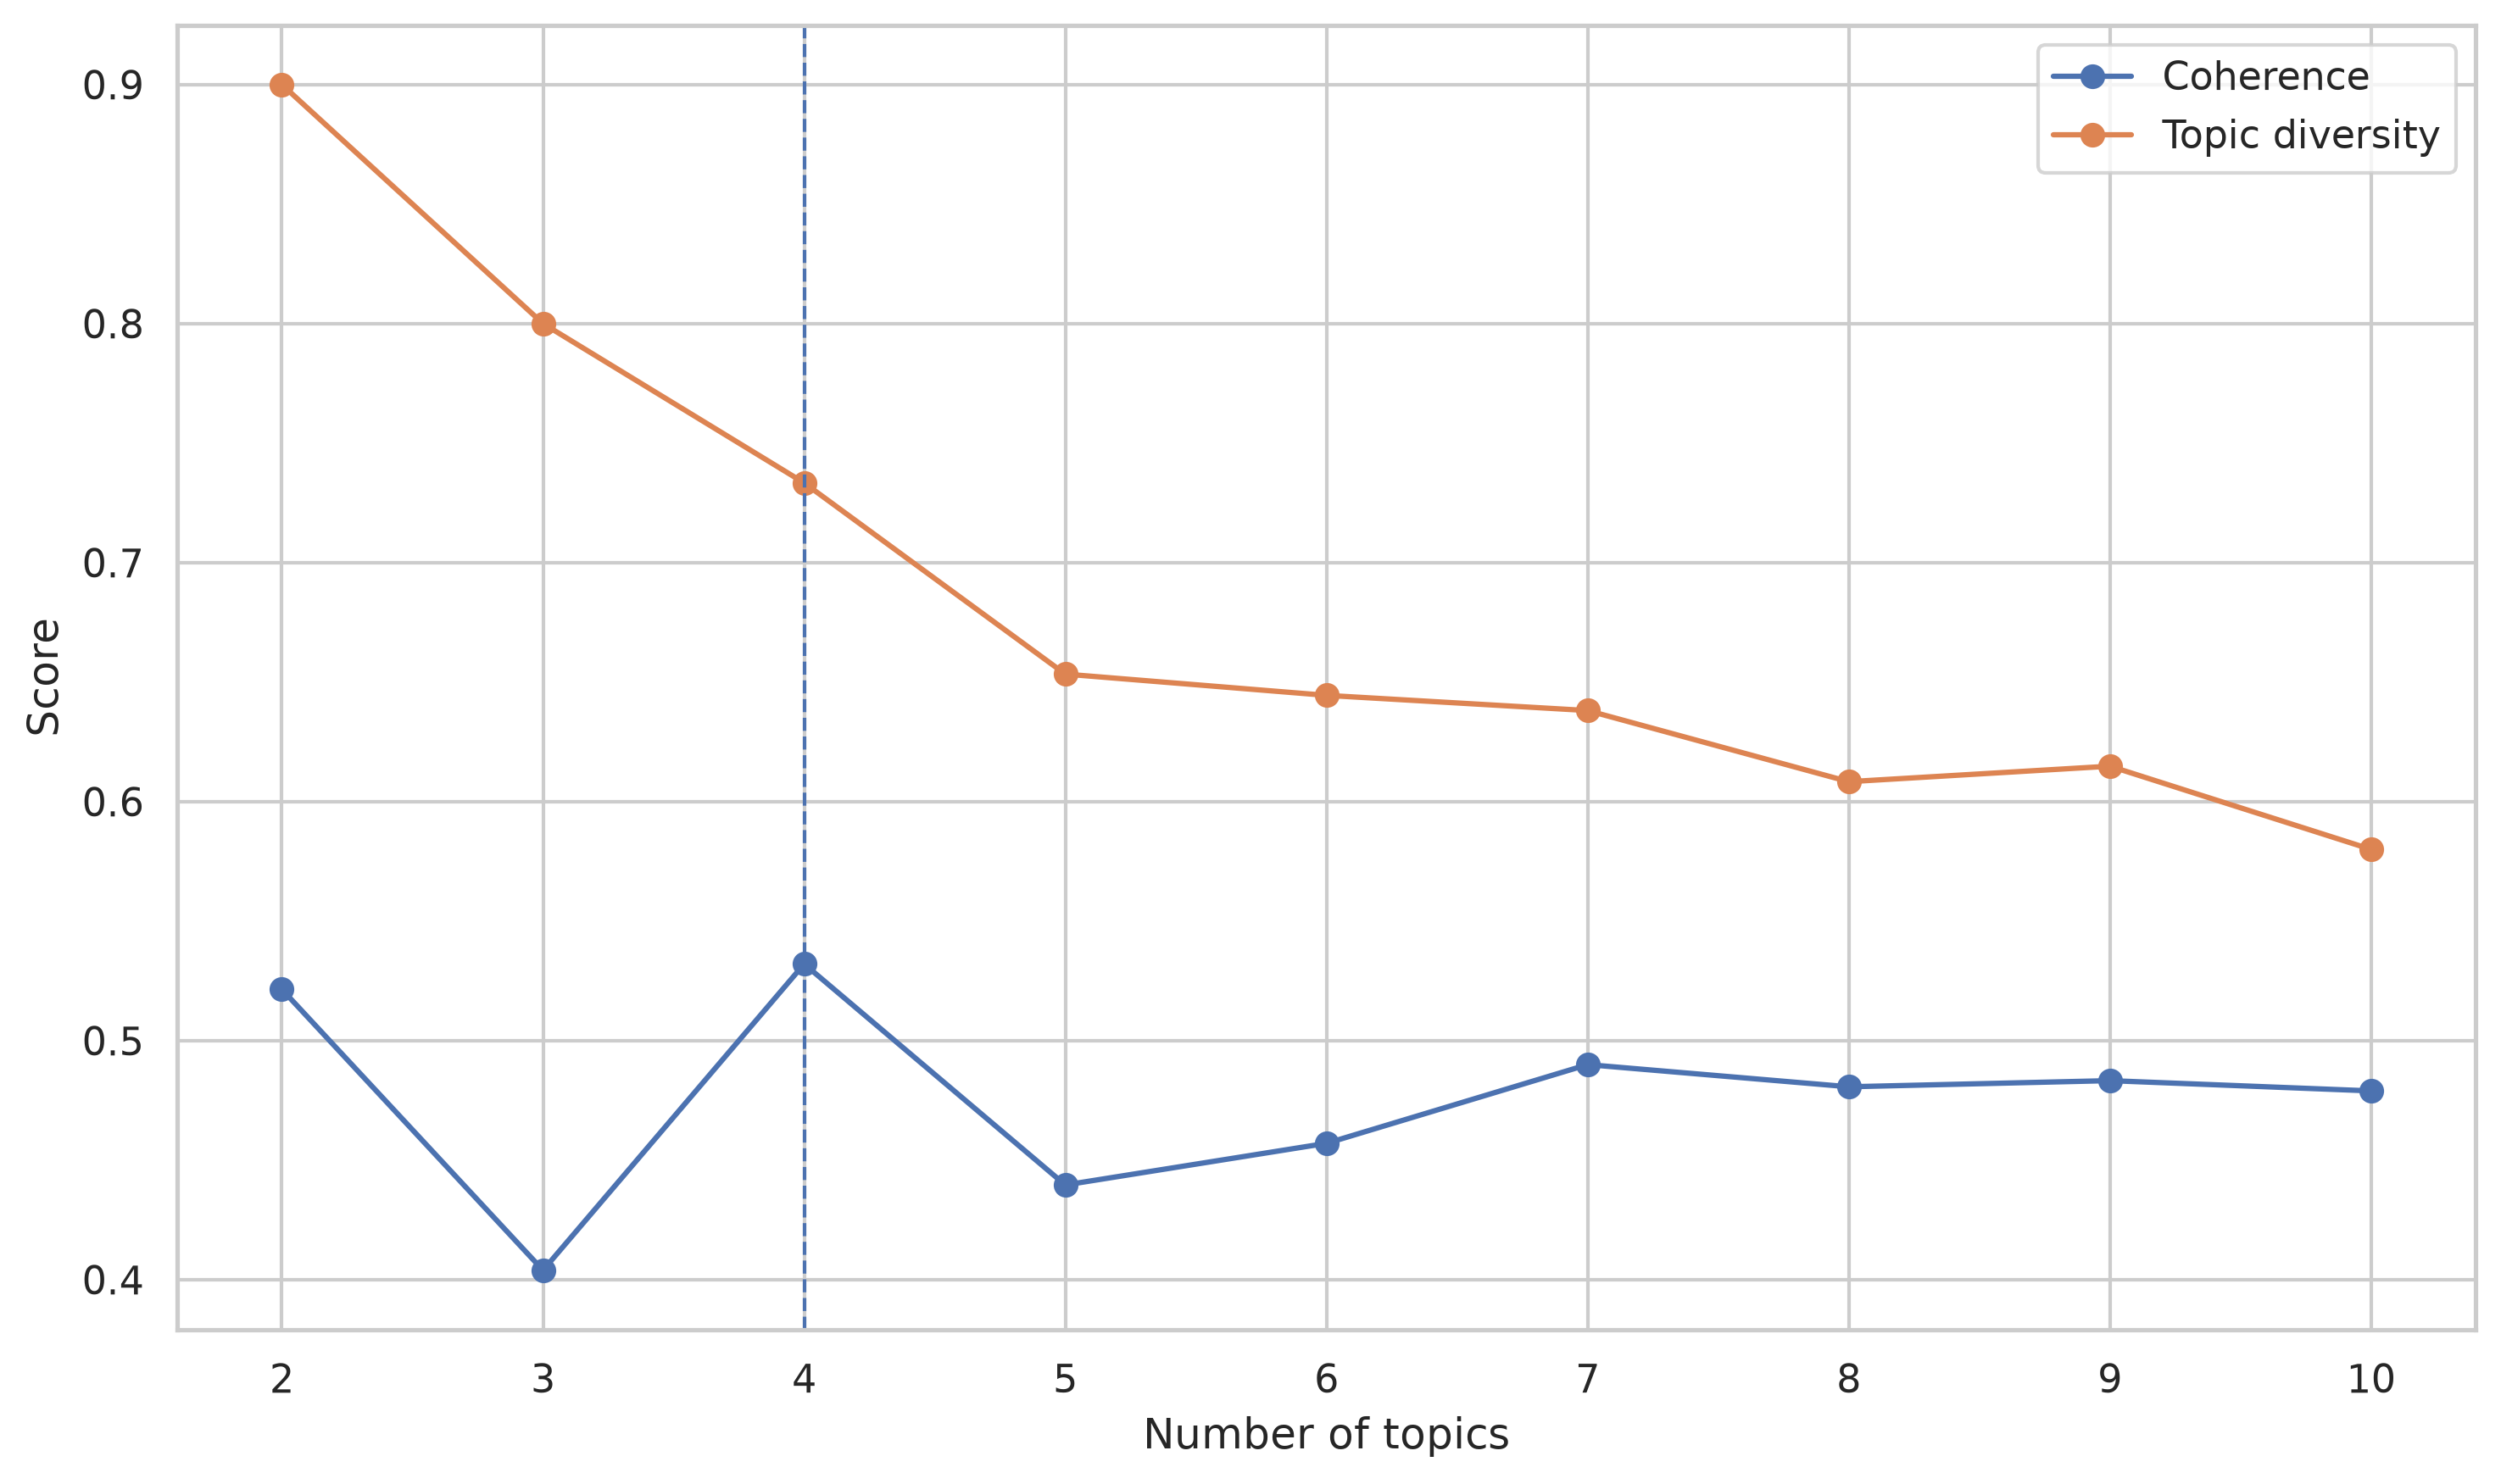
\includegraphics[width=\linewidth]{lda_sentiment_synthetic_coherence_diversity.png}
  \caption{Synthetic sentiment search.}
  \label{fig:impl-lda-synthetic-search}
\end{subfigure}
\caption{LDA coherence and diversity diagnostics for the policy, original-sentiment,
and synthetic-sentiment models.}
\label{fig:impl-lda-searches}
\end{figure}

\begin{table}[!htbp]
\centering
\small
\begin{tabular}{
  >{\centering\arraybackslash}p{0.05\linewidth}
  >{\raggedright\arraybackslash}p{0.82\linewidth}
}
\hline
Topic & Main terms \\
\hline
0 & privacy, staff, content, educator, bias, guidance, decision, potential,
principle, risk \\
1 & competency, knowledge, skill, curriculum, framework, professional,
ethic, pedagogical \\
2 & child, strategy, framework, literacy, research, public, guidance, learner,
regulation \\
3 & usage, outils, cadre, donn\'{e}es, p\'{e}dagogique, num\'{e}rique,
utilisation, d\'{e}ploiement \\
\hline
\end{tabular}
\caption{Global policy LDA topics.}
\label{tab:impl-lda-policy-topics}
\end{table}



Of 1,843 policy chunks, 1,724 were retained: {\color{blue}115 were removed because
fewer than 30 processed tokens remained after cleaning and lemmatisation, and four
exact processed-text duplicates were excluded.} The retained global
{\color{blue}model} contained four topics, with coherence of 0.7021 and diversity
of 0.9000. Figure~\ref{fig:impl-lda-searches} presents the
{\color{blue}candidate searches}, while
Table~\ref{tab:impl-lda-policy-topics} lists the retained
{\color{blue}topics}.

{\color{blue}Country-specific models retained three topics for Australia, two for
France and Ireland, and seven for the USA. Principal terms also varied across
countries. Australian topics emphasised cognitive, privacy, assessment, risk; French
topics research, innovation, pedagogical deployment; Irish topics regulation, safety,
assessment, literacy; USA topics privacy, bias, equity, assessment, guidance.}


For sentiment, the original corpus was modelled separately before synthetic data
were added. {\color{blue}Figure~\ref{fig:impl-lda-searches} shows two topics for the
original corpus and four for the combined corpus, indicating that synthetic
augmentation altered the recovered thematic structure.}
Table~\ref{tab:impl-lda-sentiment-comparison} records the resulting topic counts
and main terms.

\begin{table}[!htbp]
\centering
\small
\begin{tabular}{
  >{\raggedright\arraybackslash}p{0.2\linewidth}
  >{\centering\arraybackslash}p{0.1\linewidth}
  >{\raggedright\arraybackslash}p{0.5\linewidth}}
\hline
Subset & Topics & Main terms \\
\hline
Original sentiment & 3 & ethics, skills, social perception, experience, learning
pathways \\
Synthetic sentiment & 4 & protection, negative sentiment, integrity, access, fear,
trust, governance \\
\hline
\end{tabular}
\caption{LDA sentiment results; full topic terms are available under \texttt{LDA-S} in Table~4.1.}
\label{tab:impl-lda-sentiment-comparison}
\end{table}


LDA recovered recognisable broad themes and provided a transparent lexical
baseline. Its policy components nevertheless combined some governance,
pedagogical, and institutional concerns, while one component reflected both French
vocabulary and source concentration. The separately fitted original and synthetic
sentiment models also produced different topic counts. BERTopic-style clustering was
therefore implemented as a second view that assigned every retained chunk to a more
granular cluster.

\subsection{BERTopic-Style Clustering Results}
\label{subsec:impl-bertopic}

As defined in Subsection~\ref{subsec:method-bertopic}, the BERTopic-style
configuration combined TF--IDF, truncated {\color{blue}Singular Value Decomposition
(SVD)}, K-means, and class-based TF--IDF. {\color{blue}\cite{deerwester1990indexing} use SVD to reduce high-dimensional representations
to latent components. \cite{macqueen1967methods} introduced K-means, which
partitions vectors around $k$ centroids.} K-means replaced density-based clustering
to provide fixed topic counts, complete assignments, stable identifiers, reproducible
country distributions, and synthetic projection. Class-based TF--IDF produced
representative terms. BERTopic supplied the cluster-level representation, while
transformer embeddings, UMAP, and HDBSCAN were excluded.

Earlier transformer-based trials did not produce a more stable topic structure during
model selection. This result aligns with~\cite{antoniak2018evaluating}, who show that
embedding-based similarities can vary across small corpora,
and~\cite{yang2021language}, who find that multilingual representations retain
language-specific signals. In this heterogeneous corpus, they also captured
institutional style and report format alongside policy distinctions rather than
purely semantic topic content.

\begin{verbatim}
Policy or original sentiment chunks
  -> clean, tokenise, and filter the text
  -> build a TF-IDF document representation
  -> reduce and normalise it using truncated SVD
  -> fit candidate K-means cluster solutions
  -> compare coherence, silhouette, balance, and diversity
  -> retain the selected topic count
  -> fit BERTopic with K-means and class-based TF-IDF
  -> extract keywords and representative chunks
  -> generate and review SLM topic phrases
  -> export assignments, labels, and topic distributions
\end{verbatim}

For the synthetic robustness check, synthetic sentiment chunks were projected using
the TF--IDF vectoriser and SVD model fitted on the original sentiment corpus.
K-means then assigned each chunk to one of the retained original-sentiment topics.

\begin{samepage}
\begin{verbatim}
Synthetic sentiment chunks
  -> apply the original sentiment preprocessing rules
  -> transform with the fitted TF-IDF vectoriser
  -> transform with the fitted SVD model
  -> assign each chunk to an existing K-means topic
  -> attach the reviewed topic labels
  -> compare original and synthetic topic shares
\end{verbatim}
\end{samepage}

\begin{table}[ht]
\centering
\small
\setlength{\tabcolsep}{4pt}
\begin{tabular}{crrrrr}
\hline
Topics & Coherence & Silhouette & Balance & Diversity & Score \\
\hline
\textbf{8} & \textbf{0.1083} & 0.1297 & 0.7585 & \textbf{0.9063} &
\textbf{0.6921} \\
9 & 0.1060 & \textbf{0.1370} & \textbf{0.7961} & 0.8704 & 0.6576 \\
\hline
\end{tabular}
\caption{Policy BERTopic candidate metrics.}
\label{tab:impl-bertopic-policy-candidates}
\end{table}


\subsubsection*{Policy BERTopic Results}

The policy search compared eight- and nine-topic candidates. The eight-topic
solution obtained a combined score of 0.6921, compared with 0.6576 for the
nine-topic solution, and was retained for the reported outputs after comparative
metric review. Table~\ref{tab:impl-bertopic-policy-candidates} gives the candidate
metrics.

\begin{figure}[!htbp]
\centering
\begin{minipage}[t]{0.49\linewidth}
 \centering
 
\includegraphics[width=\linewidth]
 {bert_policy_global_topic_selection_metrics.png}
 \vspace{-0.5em}
 {\scriptsize (a) Candidate diagnostics.}
\end{minipage}\hfill
\begin{minipage}[t]{0.49\linewidth}
 \centering
 
\includegraphics[width=\linewidth]
 {bert_policy_global_topic_distribution_by_country.png}
 \vspace{-0.5em}
 {\scriptsize (b) Topic distribution by country.}
\end{minipage}
\caption{Policy BERTopic results for the retained eight-topic model.}
\label{fig:impl-bertopic-policy}
\end{figure}

The retained topic shares and reviewed report labels are listed in
Table~\ref{tab:impl-bertopic-policy-topics}. The labels were produced after
clustering from the keywords and representative chunks and did not affect the model
outputs.

\begin{table}[!htbp]
\centering
\small
\begin{tabular}{
  >{\centering\arraybackslash}p{0.08\linewidth}
  >{\raggedright\arraybackslash}p{0.12\linewidth}
  >{\raggedright\arraybackslash}p{0.68\linewidth}
}
\hline
Topic & Share & Reviewed topic label \\
\hline
0 & 0.242 & Artificial intelligence impact on educational practices \\
1 & 0.192 & AI teacher-assistant oversight and curriculum alignment \\
2 & 0.141 & AI-powered learning platforms and student privacy \\
3 & 0.113 & AI in school curriculum and teacher training \\
4 & 0.105 & AI competency-framework design and ethical application \\
5 & 0.094 & Child protection and digital-education oversight \\
6 & 0.076 & AI-powered digital-learning strategies for youth \\
7 & 0.037 & Cognitive offloading and metacognitive skills in education \\
\hline
\end{tabular}
\caption{Retained global policy BERTopic topics and reviewed labels.}
\label{tab:impl-bertopic-policy-topics}
\end{table}

The global model supplied a shared country--topic matrix, while separate country
models produced local topic structures. Australia retained six topics, France eight,
Ireland four, and the USA seven. Table~\ref{tab:impl-bertopic-policy-countries}
reports the principal country-level outputs used in subsequent comparisons.

\begin{table}[!htbp]
\centering
\footnotesize
\begin{tabular}{
  >{\centering\arraybackslash}p{0.12\linewidth}
  >{\centering\arraybackslash}p{0.10\linewidth}
  >{\raggedright\arraybackslash}p{0.68\linewidth}
}
\hline
Country & Topics & Main country-specific topics and shares \\
\hline
Australia & 6 & Curriculum-development oversight (22.7\%); cognitive offloading
and metacognition (18.9\%); academic-integrity guidance for generative AI (16.4\%);
followed by ethics, governance, and an Australian school-AI framework. \\
France & 8 & National AI-strategy implementation in education (20.9\%); school
curriculum and teacher training (19.0\%); curriculum integration (18.4\%);
personalised learning (13.2\%); followed by research funding, regulation, and digital
leadership. \\
Ireland & 4 & Public AI governance and oversight (35.5\%); digital-learning
framework implementation and teacher development (34.8\%); staff AI use and academic
responsibility (16.8\%); child protection (12.9\%). \\
USA & 7 & AI-supported assessment and feedback (17.7\%); educational-tool
oversight (17.1\%); curriculum and teacher training (16.7\%); student privacy
(15.4\%); followed by district policy and further curriculum topics. \\
\hline
\end{tabular}
\caption{Country-level policy BERTopic outputs.}
\label{tab:impl-bertopic-policy-countries}
\end{table}


The country-level models reveal differences in thematic concentration across the
national corpora. Ireland produced the most concentrated structure, with governance
and digital-learning implementation accounting for most chunks, whereas France and
Australia required more granular topic spaces covering strategy, curriculum,
training, integrity, and cognitive effects. The USA showed a broader distribution
across assessment, tool oversight, teacher preparation, and privacy. These outputs
describe differences in corpus emphasis and should not be interpreted as direct
measures of national policy maturity or effectiveness.

\subsubsection*{Sentiment BERTopic Results}

The original sentiment search compared eight-, nine-, and ten-topic candidates. The
nine-topic solution had the highest coherence and combined score, with
{\color{blue}qualitative review confirming clearer topic separation.}
Figure~\ref{fig:impl-bertopic-sentiment-results}(a) shows selection diagnostics;
candidate metrics appear in
Table~\ref{tab:impl-bertopic-sentiment-candidates}.

Synthetic chunks were assigned to the retained nine-topic original-sentiment space.
Their topic shares and differences across both sets are shown in
Figure~\ref{fig:impl-bertopic-sentiment-results}(b)--(c) and reported in
Table~\ref{tab:impl-bertopic-synthetic-topics}. The mean absolute topic-share
difference was 8.4 percentage points. No synthetic chunks were assigned to Topics~1
or~5. These results formed the BERTopic sensitivity result. The topic shares and
reviewed SLM-assisted labels are shown in
Table~\ref{tab:impl-bertopic-sentiment-topics}.

\begin{table}[ht]
\centering
\small
\setlength{\tabcolsep}{4pt}
\begin{tabular}{crrrrr}
\hline
Topics & Coherence & Silhouette & Balance & Diversity & Score \\
\hline
8 & 0.0184 & 0.1318 & 0.7495 & 0.8125 & 0.5247 \\
\textbf{9} & \textbf{0.0538} & 0.1418 & 0.7692 & \textbf{0.8241} &
\textbf{0.8388} \\
10 & 0.0377 & \textbf{0.1442} & \textbf{0.7758} & 0.8000 & 0.6877 \\
\hline
\end{tabular}
\caption{Original sentiment BERTopic candidate metrics.}
\label{tab:impl-bertopic-sentiment-candidates}
\end{table}

The retained topics organise sentiment around three connected dimensions: classroom
use and teacher adaptation, governance and implementation, and wider youth and public
concerns. As shown in Table~\ref{tab:impl-bertopic-sentiment-topics}, Topics~0--2
represent the largest shares and emphasise educational experience, while Topics~3--6
focus on ethics, implementation, and social risks. Topics~7 and~8 capture smaller but
distinct Irish and French public perspectives. Overall, the distribution reflects
both shared educational concerns and context-specific public attitudes towards AI.


\begin{figure}[!htbp]
\centering

\begin{subfigure}[t]{0.68\linewidth}
    \centering
    
\includegraphics[scale=.26]
    {bert_sentiment_topic_selection_metrics.png}
    \caption{Topic-number selection diagnostics.}
    \label{fig:impl-bertopic-sentiment-search}
\end{subfigure}

\vspace{0.6em}

\begin{subfigure}[t]{0.49\linewidth}
    \centering
    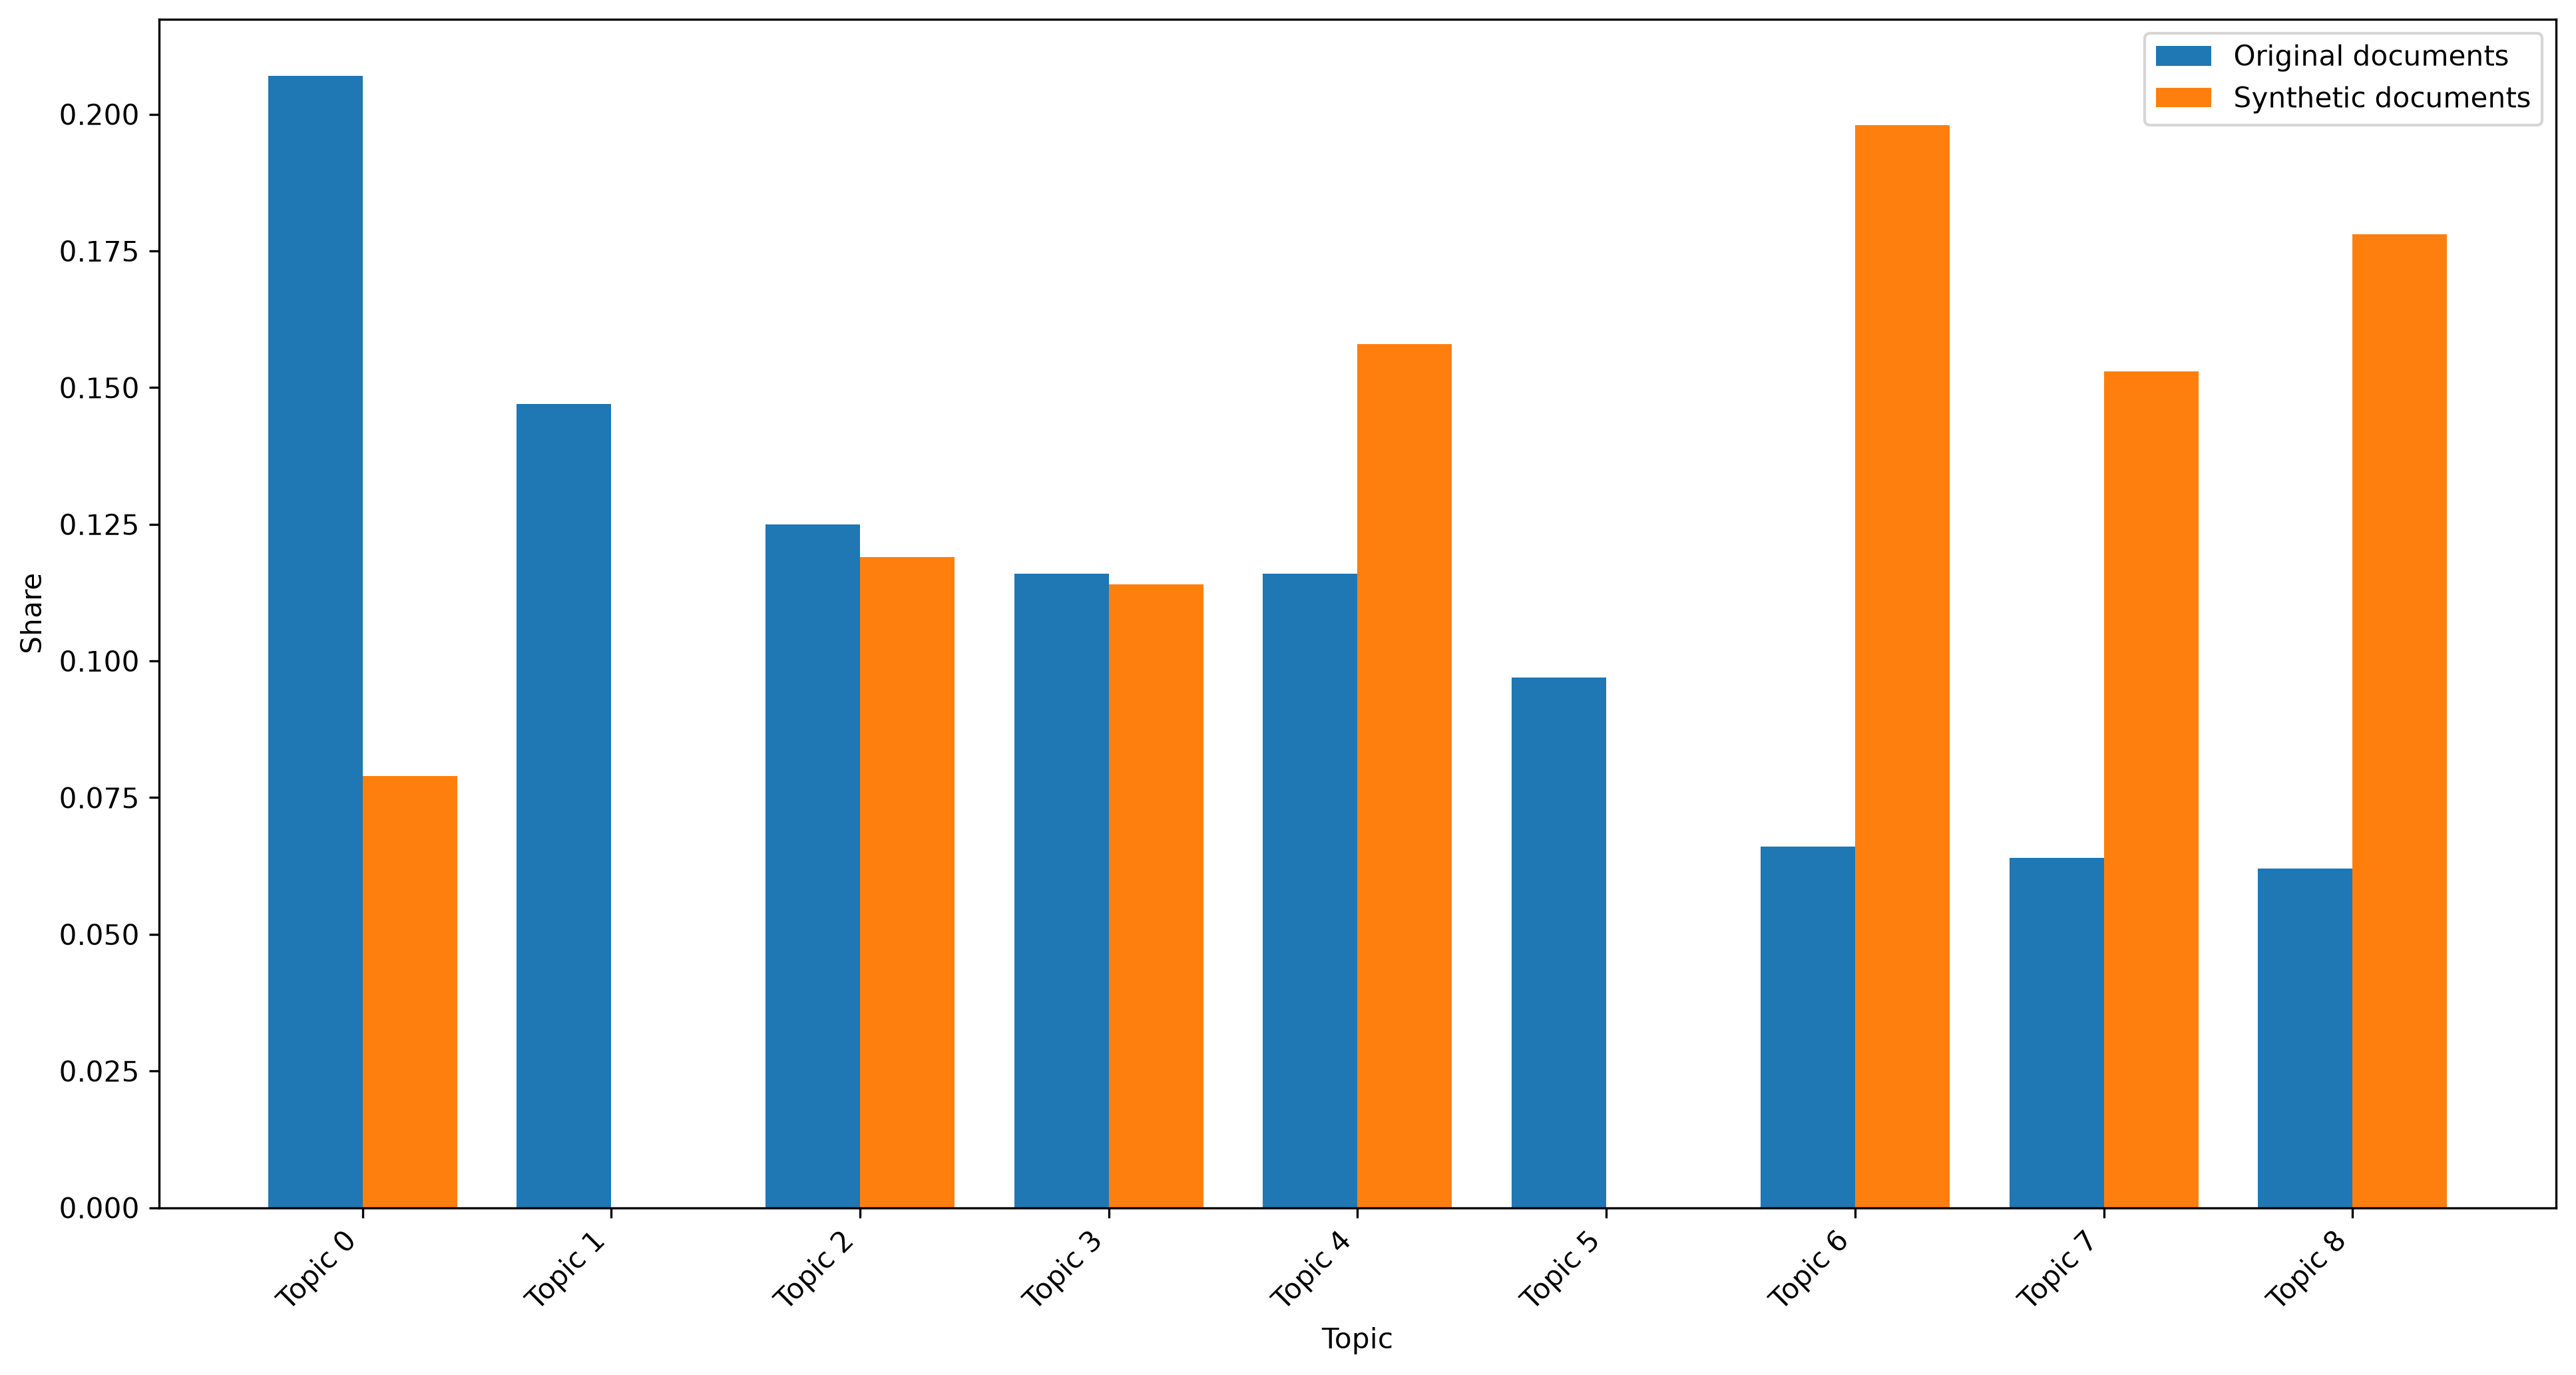
\includegraphics[scale=.21]
    {bert_sentiment_original_vs_synthetic_distribution.png}
    \caption{Original and synthetic topic shares.}
    \label{fig:impl-bertopic-synthetic-distribution}
\end{subfigure}
\hfill
\begin{subfigure}[t]{0.49\linewidth}
    \centering
    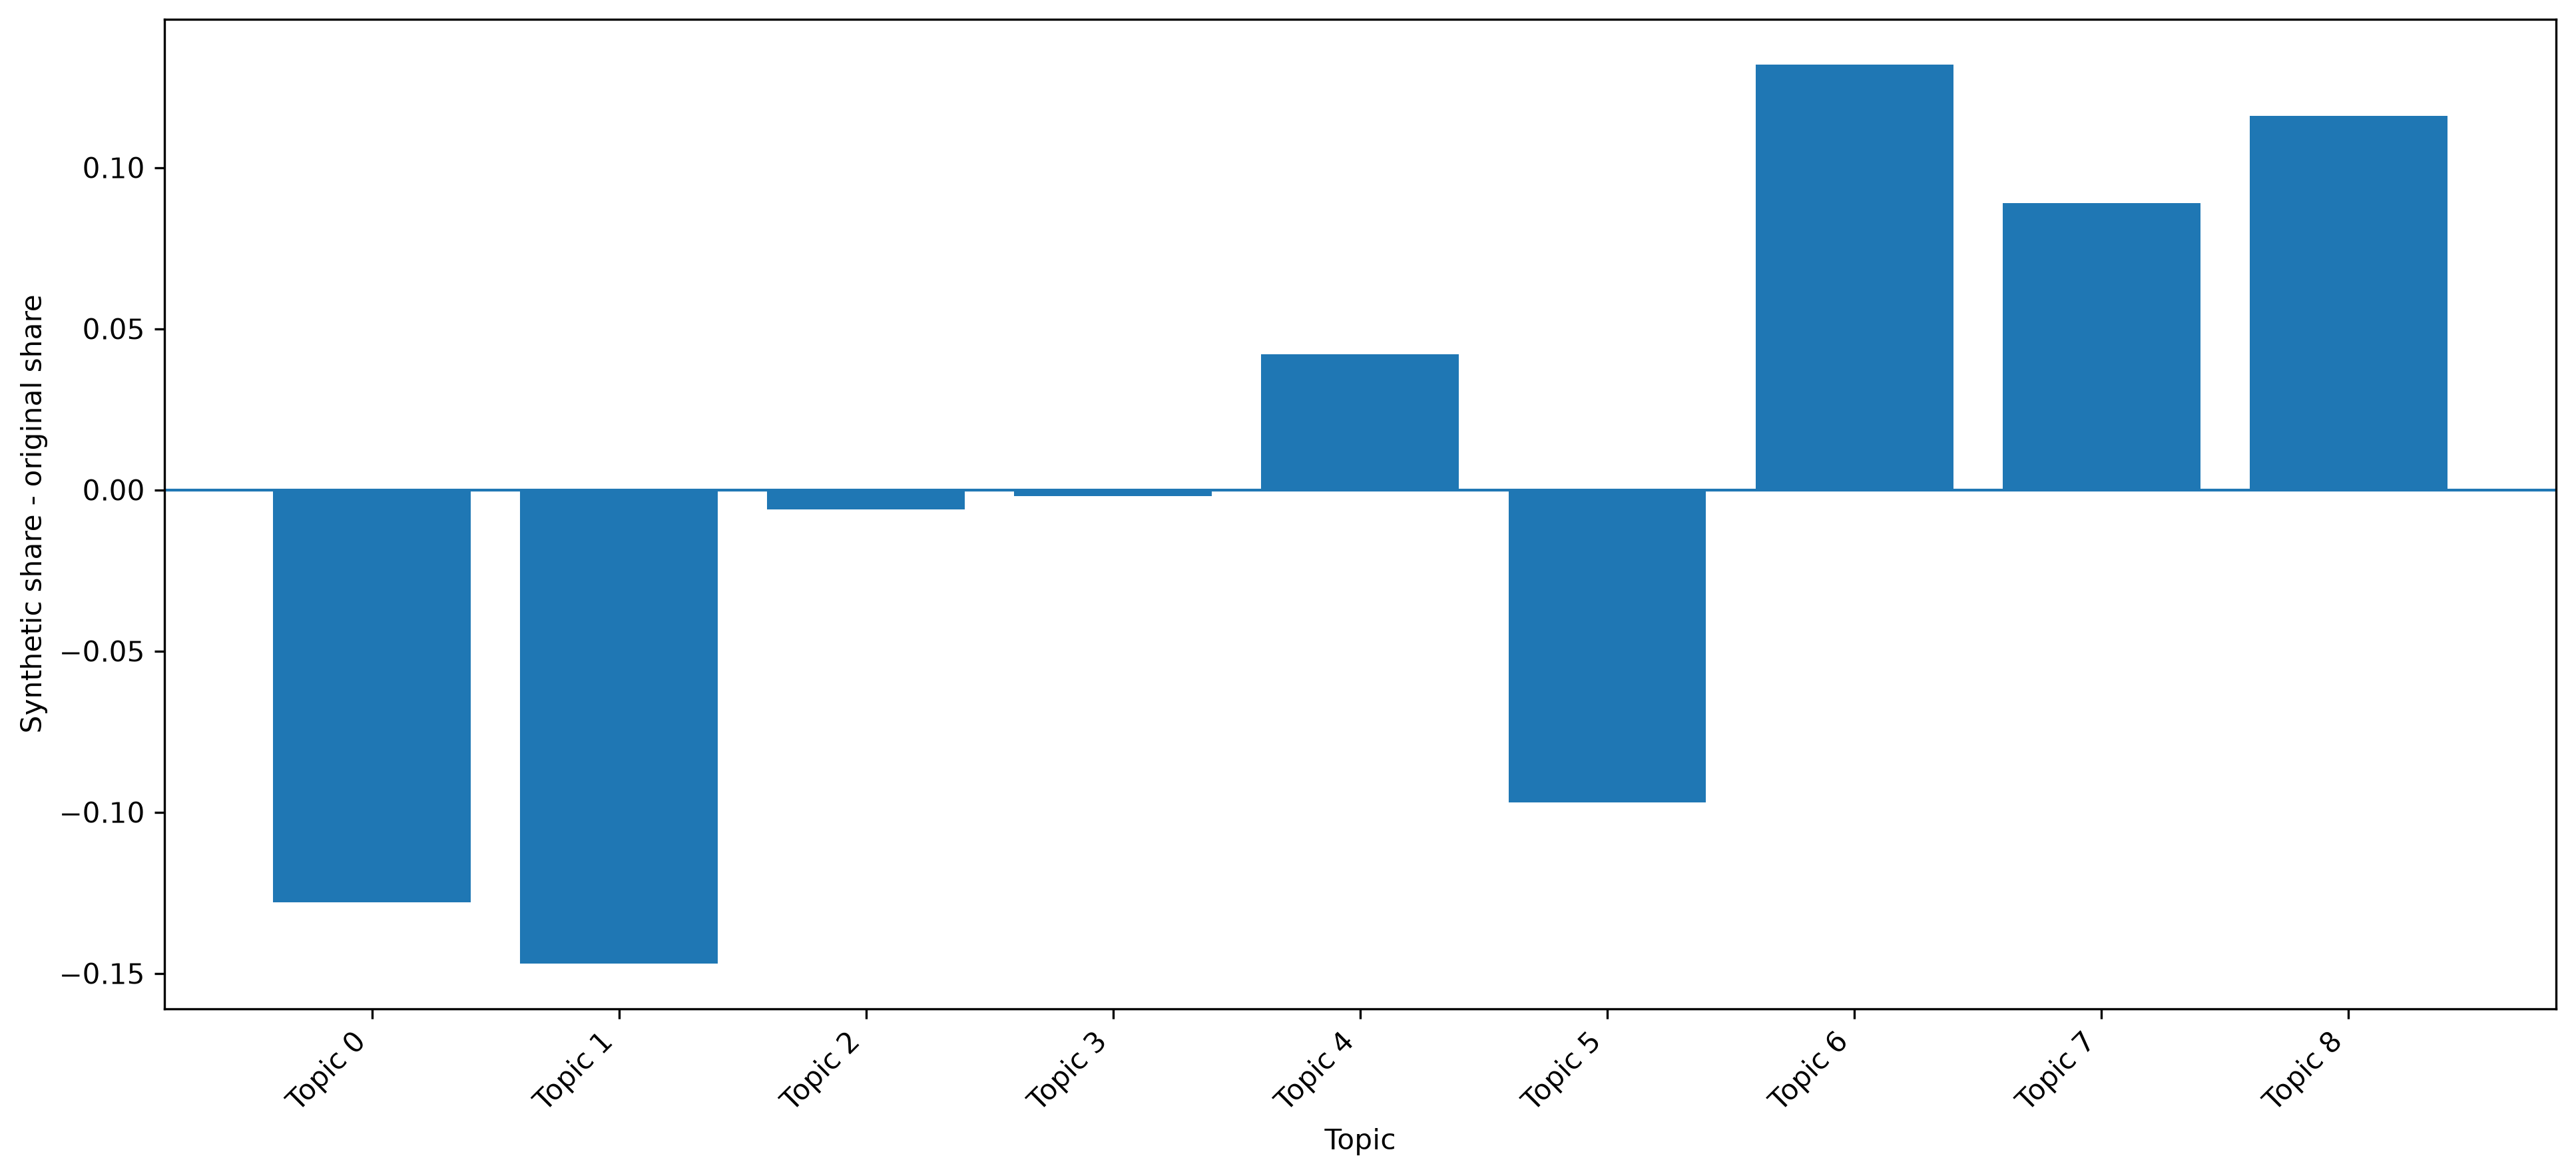
\includegraphics[scale=.22]
    {bert_sentiment_synthetic_share_difference.png}
    \caption{Synthetic minus original share.}
    \label{fig:impl-bertopic-synthetic-difference}
\end{subfigure}

\caption{Sentiment BERTopic model selection and synthetic-sentiment robustness
results.}
\label{fig:impl-bertopic-sentiment-results}
\end{figure}


\begin{table}[!htbp]
\centering
\small
\begin{tabular}{
>{\raggedright\arraybackslash}p{0.08\linewidth}
>{\raggedright\arraybackslash}p{0.12\linewidth}
>{\raggedright\arraybackslash}p{0.68\linewidth}
}
\hline
Topic & Share & Reviewed topic label \\
\hline
0 & 0.207 & Student and classroom AI use: benefits and concerns \\
1 & 0.147 & Teacher adaptation and professional learning for AI \\
2 & 0.125 & AI4T professional-learning experiences and perceptions \\
3 & 0.116 & Ethics and governance frameworks for AI in education \\
4 & 0.116 & Youth-sector AI opportunities and governance risks \\
5 & 0.097 & Child and youth concerns about AI-related social harm \\
6 & 0.066 & Staff and learner concerns about GenAI implementation \\
7 & 0.064 & Irish public fears and hopes about AI \\
8 & 0.062 & French public views on AI regulation, risks, and benefits \\
\hline
\end{tabular}
\caption{Original sentiment BERTopic topics and reviewed labels.}
\label{tab:impl-bertopic-sentiment-topics}
\end{table}

\begin{table}[!htbp]
\centering
\scriptsize
\begin{tabular}{
>{\raggedright\arraybackslash}p{0.06\linewidth}
>{\raggedright\arraybackslash}p{0.45\linewidth}
rrr
}
\hline
Topic & Short label & Original & Synthetic & Difference \\
\hline
0 & Classroom AI use & 20.7\% & 7.9\% & $-12.8$ pp \\
1 & Teacher adaptation & 14.7\% & 0.0\% & $-14.7$ pp \\
2 & AI4T professional learning & 12.5\% & 11.9\% & $-0.6$ pp \\
3 & Ethics and governance & 11.6\% & 11.4\% & $-0.2$ pp \\
4 & Youth-sector risks and opportunities & 11.6\% & 15.8\% & $+4.2$ pp \\
5 & Child and youth social harm & 9.7\% & 0.0\% & $-9.7$ pp \\
6 & GenAI implementation concerns & 6.6\% & 19.8\% & $+13.2$ pp \\
7 & Irish public fears and hopes & 6.4\% & 15.3\% & $+8.9$ pp \\
8 & French public risks and benefits & 6.2\% & 17.8\% & $+11.6$ pp \\
\hline
\end{tabular}
\caption{Original and synthetic sentiment shares in the fitted BERTopic space;
``pp'' denotes percentage points.}
\label{tab:impl-bertopic-synthetic-topics}
\end{table}

BERTopic supplied a clustering-based comparison and topic space for the synthetic
check. {\color{blue}The mean absolute difference between original and synthetic
topic shares was 8.4 percentage points}, and two sentiment topics received no
synthetic assignments. NMF was then implemented {\color{blue}as a
factorisation-based model to test whether the representation provided broader
thematic continuity.}

\subsection{NMF Factorisation Results}
\label{subsec:impl-nmf}

As defined in Subsection~\ref{subsec:method-nmf}, NMF factorised TF--IDF into
document--topic and topic--term matrices. {\color{blue}NNDSVDa initialisation,
which fills zero entries of NNDSVD with the input-matrix mean, followed the
SVD-based approach of Boutsidis and Gallopoulos~\cite{boutsidis2008svd}.
Coordinate descent was used to optimise the factor matrices, as described
by Hsieh and Dhillon~\cite{hsieh2011fast}, while Frobenius loss measured
reconstruction error, following the NMF formulation of Lee and
Seung~\cite{lee1999learning}.} A seed of 42 and 1000 iterations were used.

{\small
\begin{verbatim}
Policy or original sentiment chunks
  -> clean, tokenise, and filter the text
  -> build a unigram-and-bigram TF-IDF matrix
  -> fit candidate NMF factorisations
  -> assign each chunk to its highest-weight component
  -> compare candidate metrics and diagnostic outputs
  -> retain and fit the selected topic count
  -> export document-topic and topic-term matrices
  -> extract keywords and representative chunks
  -> generate and review SLM topic phrases
  -> export assignments, labels, and distributions
\end{verbatim}
}

For the synthetic check defined in
Subsection~\ref{subsec:method-synthetic-robustness}, synthetic sentiment was
transformed using the TF--IDF vectoriser and NMF model fitted on original sentiment.
Each synthetic chunk was assigned to its highest-weight topic.

{\small
\begin{verbatim}
Synthetic sentiment chunks
  -> apply the original sentiment preprocessing rules
  -> transform with the fitted TF-IDF vectoriser
  -> transform with the fitted NMF model
  -> assign each chunk to its highest-weight topic
  -> attach the reviewed topic labels
  -> compare original and synthetic topic shares
\end{verbatim}
}

\begin{table}[ht]
\centering
\small
\setlength{\tabcolsep}{4pt}
\begin{tabular}{crrrrr}
\hline
Topics & Coherence & Silhouette & Balance & Diversity & Score \\
\hline
8 & 0.0903 & \textbf{0.6875} & 0.8231 & 0.9167 & 0.5921 \\
\textbf{9} & \textbf{0.0953} & 0.6685 & \textbf{0.8533} &
\textbf{0.9167} & \textbf{0.6549} \\
10 & 0.0831 & 0.6626 & 0.8469 & 0.9083 & 0.4620 \\
\hline
\end{tabular}
\caption{Policy NMF candidate metrics.}
\label{tab:impl-nmf-policy-candidates}
\end{table}

\begin{figure}[!htbp]
\centering
\vspace*{-.25cm}
\begin{minipage}[t]{0.49\linewidth}
 \centering
 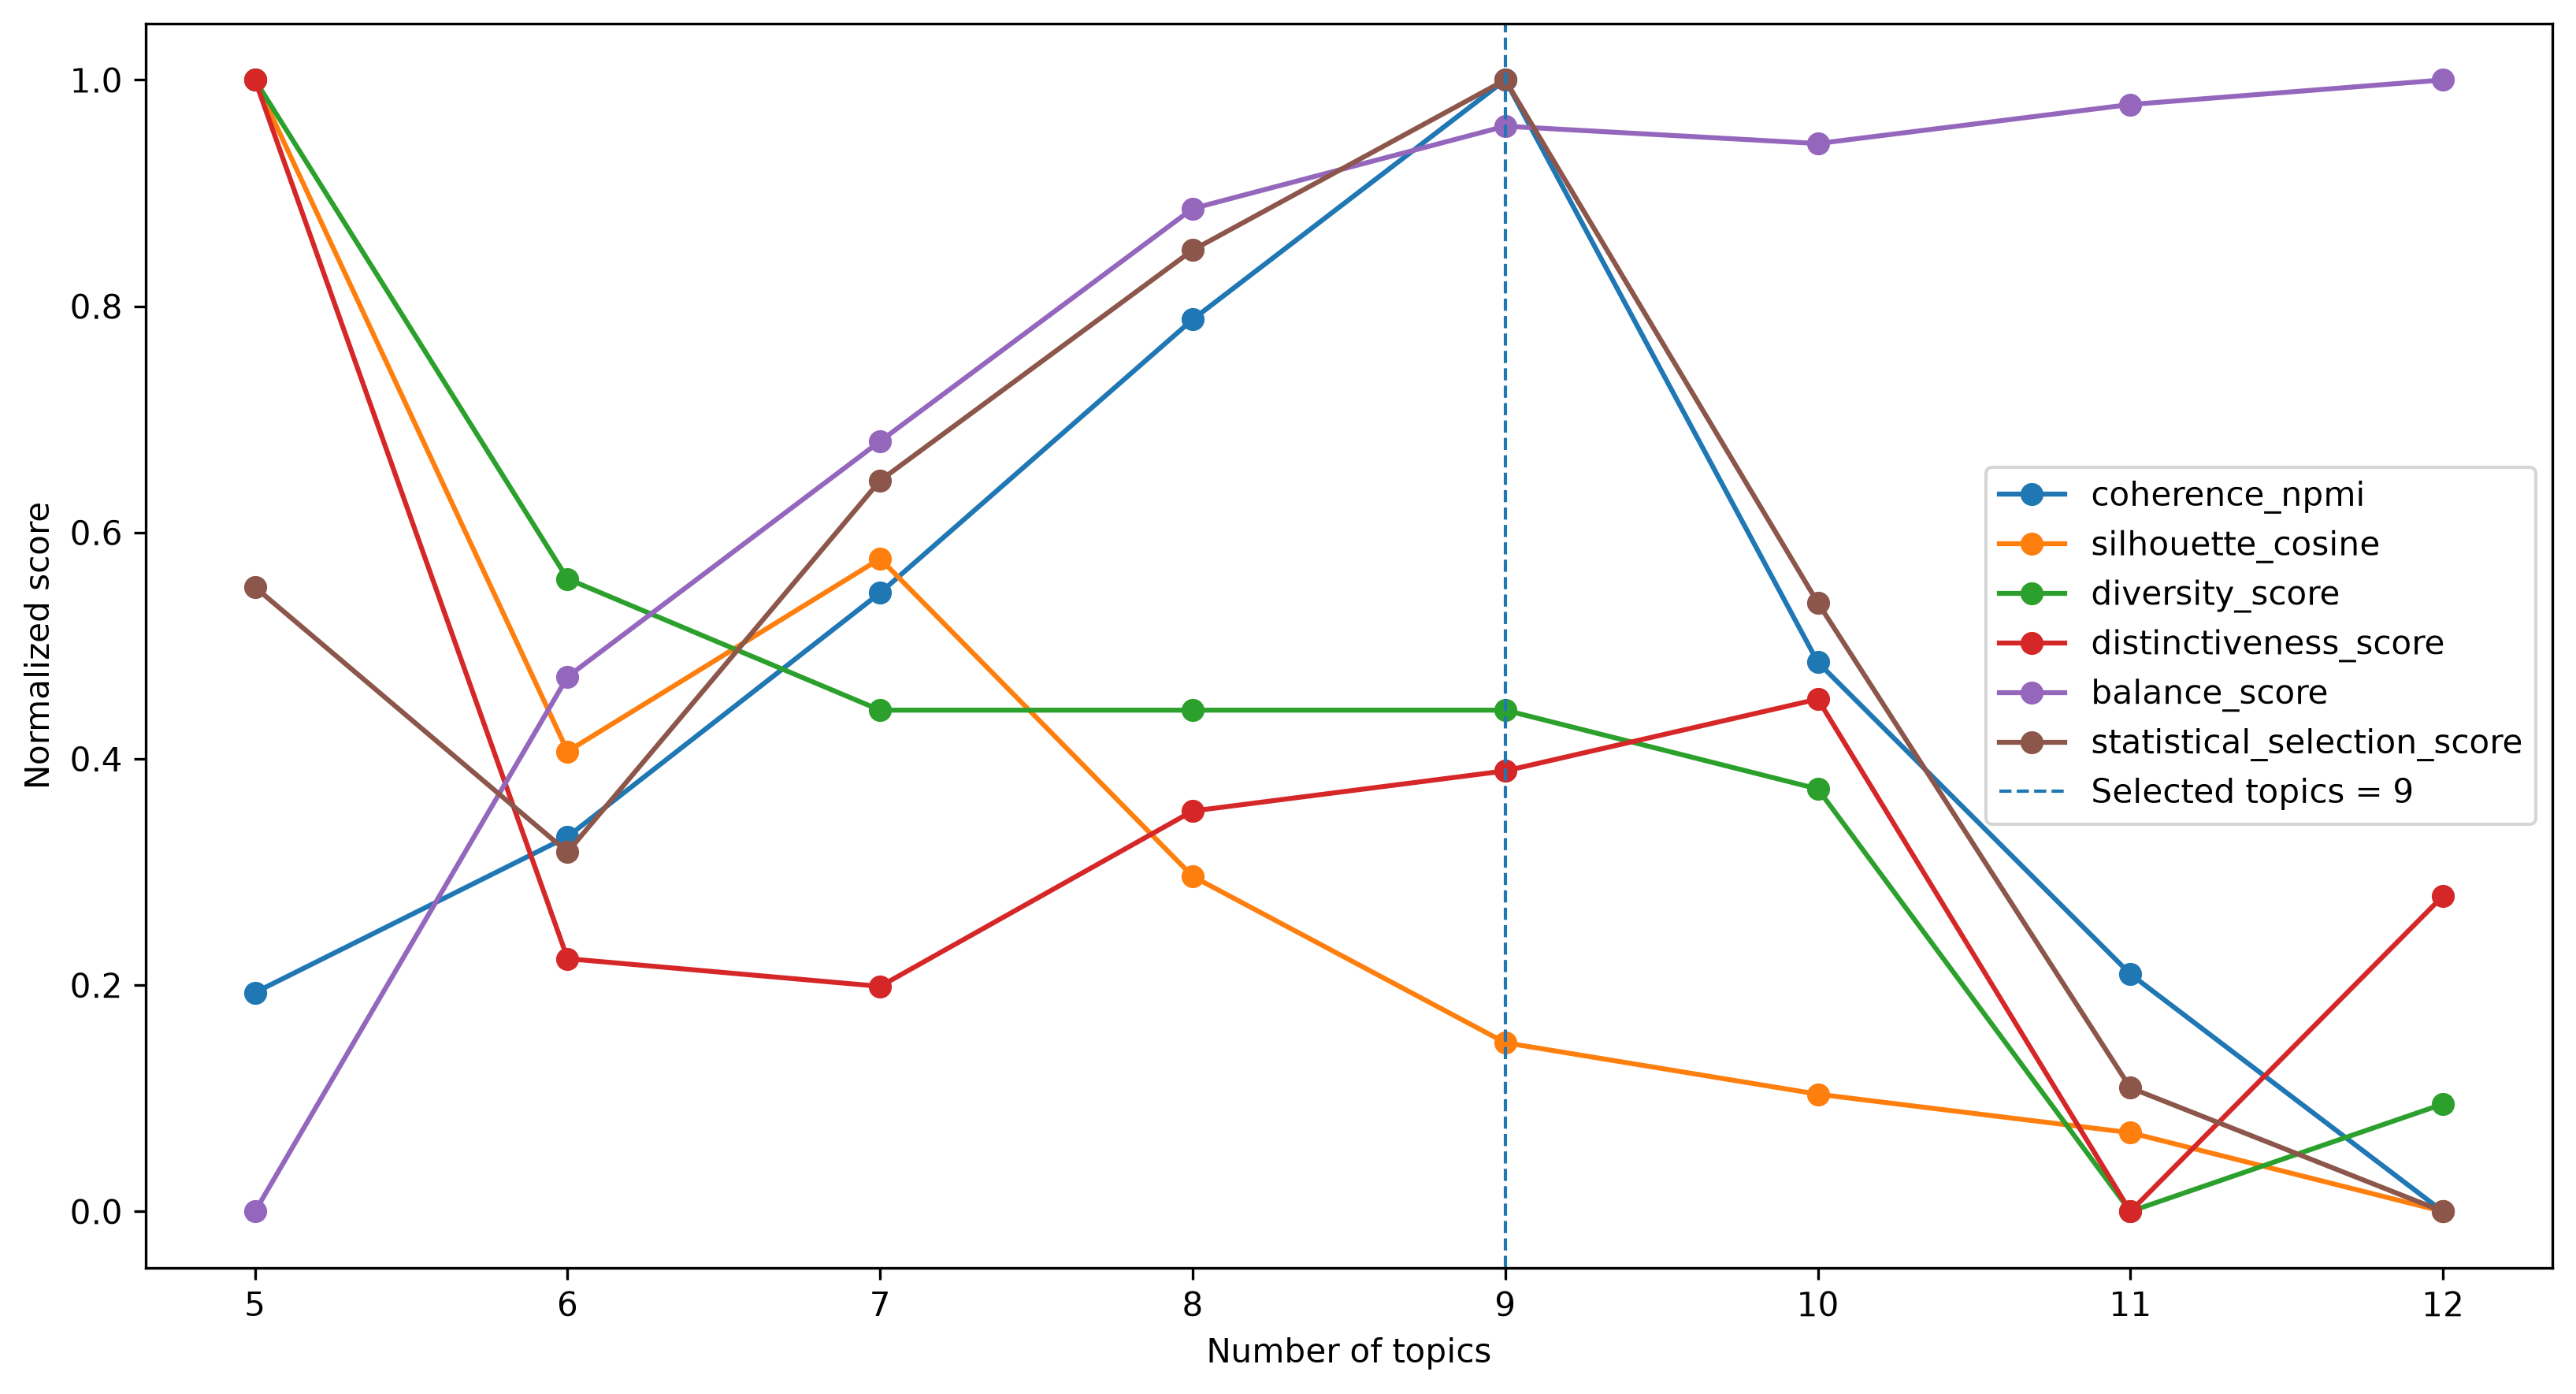
\includegraphics[width=\linewidth]
 {policy_global_nmf_topic_selection_metrics.png}
 \vspace{-0.5em}
 {\scriptsize (a) Topic-number diagnostics.}
\end{minipage}\hfill
\begin{minipage}[t]{0.49\linewidth}
 \centering
 
\includegraphics[scale=.2]
 {policy_global_nmf_topic_distribution_by_country.png}\\
 \vspace{-0.5em}
 {\scriptsize (b) Topic distribution by country.}
\end{minipage}
\caption{Policy NMF results for the retained nine-topic model.}
\label{fig:impl-nmf-policy}
\vspace*{-.25cm}
\end{figure}


\subsubsection*{Policy NMF Results}

The policy search compared eight-, nine-, and ten-topic candidates. The nine-topic
solution obtained the highest coherence and combined score and was retained.
{\color{blue}Qualitative review also supported nine topics: it separated
privacy and ethical governance from educator guidance and professional development,
whereas eight merged these themes and ten introduced further fragmentation.}
The candidate results are shown in Figure~\ref{fig:impl-nmf-policy} and
Table~\ref{tab:impl-nmf-policy-candidates}. The retained policy-topic shares and
reviewed SLM-assisted labels are listed in
Table~\ref{tab:impl-nmf-policy-topics}.
\begin{table}[!htbp]
\centering
\small
\begin{tabular}{>{\raggedright\arraybackslash}p{0.08\linewidth}>{\raggedright\arraybackslash}p{0.12\linewidth}>{\raggedright\arraybackslash}p{0.68\linewidth}}
\hline
Topic & Share & Reviewed topic label \\
\hline
0 & 0.147 & AI-assisted learning-assessment protocols \\
1 & 0.079 & AI child protection and rights \\
2 & 0.116 & AI usage and pedagogy in school governance \\
3 & 0.105 & AI competency-framework and curriculum development \\
4 & 0.048 & Cognitive offloading in AI-assisted education \\
5 & 0.102 & Digital-learning frameworks and assessment policies \\
6 & 0.147 & AI ethical guidelines and school-data protection \\
7 & 0.131 & AI educator guidance and professional development \\
8 & 0.125 & AI curriculum development and school oversight \\
\hline
\end{tabular}
\caption{Global policy NMF topics and reviewed labels.}
\label{tab:impl-nmf-policy-topics}
\vspace*{-.25cm}
\end{table}

\vspace*{-.25cm}
The global NMF model supplied the country--topic matrix, while separate national
models produced local topic structures. Australia retained three topics, France
seven, Ireland four, and the USA seven. Table~\ref{tab:impl-nmf-policy-countries}
reports the country-level outputs.

\begin{table}[!htbp]
\centering
\footnotesize
\begin{tabular}{
  >{\centering\arraybackslash}p{0.12\linewidth}
  >{\centering\arraybackslash}p{0.10\linewidth}
  >{\raggedright\arraybackslash}p{0.68\linewidth}}
\hline
Country & Topics & Main country-specific topics and shares \\
\hline
Australia & 3 & Ethics guidelines and staff training (54.3\%); AI governance and
stakeholder engagement (23.7\%); cognitive offloading in education (22.0\%). \\
France & 7 & Educational and pedagogical AI practices (33.4\%); national
curriculum development and school coordination (18.7\%); large language models in
educational technology (13.2\%); national strategy and funding (11.0\%); followed by
regulation, school-use challenges, and digital leadership. \\
Ireland & 4 & Digital-learning framework and teacher competence (32.4\%);
child-protection regulation (24.2\%); public AI oversight and rights compliance
(23.5\%); assessment and academic misconduct (19.9\%). \\
USA & 7 & Massachusetts K--12 AI guidance (20.3\%); AI-assisted learning and
academic integrity (20.1\%); student privacy and technology oversight (18.4\%);
adaptive learning and personalised instruction (18.2\%); followed by governance,
equity, and assessment-bias topics. \\
\hline
\end{tabular}
\caption{Country-level policy NMF outputs.}
\label{tab:impl-nmf-policy-countries}
\end{table}

The country-level NMF models show clear differences in thematic concentration.
Australia produced the most concentrated structure, with ethics guidance and staff
training accounting for more than half of the corpus. Ireland divided more evenly
across teacher competence, child protection, public oversight, and academic
integrity. France and the USA required broader seven-topic structures covering
pedagogy, curriculum, strategy, regulation, privacy, equity, and assessment. These
patterns reflect differences in corpus emphasis rather than direct measures of
national policy quality or maturity.

\subsubsection*{Sentiment NMF Results}

The original sentiment search produced the highest combined score at seven topics.
Five, seven, eight, and nine topics formed a close candidate range. Nine topics were
retained after reviewing terms and representative chunks because this solution
separated teacher experience, online-learning reactions, assessment uncertainty, and
French digital-technology views merged in smaller solutions.
Figure~\ref{fig:impl-nmf-sentiment}(a) shows the statistical winner and retained
output; nine topics are not presented as the unique optimum under the statistical
criteria alone.

The topic shares and reviewed SLM-assisted labels are shown in
Table~\ref{tab:impl-nmf-sentiment-topics}. Synthetic chunks were projected into the
retained original-sentiment topic space. Their shares and differences are shown in
Figure~\ref{fig:impl-nmf-sentiment}(b)--(c) and
Table~\ref{tab:impl-nmf-synthetic-topics}. The mean absolute share difference was
5.4 percentage points, with synthetic chunks assigned to eight of nine topics. This
shift was smaller and coverage broader than BERTopic's 8.4-percentage-point shift and
seven-of-nine coverage. The fitted NMF matrices were exported for the causal NLP
pipelines.

\begin{table}[!htbp]
\centering
\small
\begin{tabular}{
>{\raggedright\arraybackslash}p{0.08\linewidth}
>{\raggedright\arraybackslash}p{0.12\linewidth}
>{\raggedright\arraybackslash}p{0.68\linewidth}
}
\hline
Topic & Share & Reviewed topic label \\
\hline
0 & 0.081 & Young people's AI impact on education and well-being \\
1 & 0.158 & Student engagement and teacher adaptation to AI \\
2 & 0.073 & GenAI detection and assessment confusion \\
3 & 0.198 & Educator training and ethical AI integration \\
4 & 0.121 & Youth workers' perspectives on AI integration \\
5 & 0.147 & Teachers' experience and knowledge in AI integration \\
6 & 0.086 & Public perceptions of AI and youth employment \\
7 & 0.073 & Online-learning intention clarity and classroom relevance \\
8 & 0.064 & French views on digital technologies, youth, and education \\
\hline
\end{tabular}
\caption{Original sentiment NMF topics and reviewed labels.}
\label{tab:impl-nmf-sentiment-topics}
\end{table}



\begin{figure}[!htbp]
\centering

\begin{subfigure}[t]{0.68\linewidth}
    \centering
    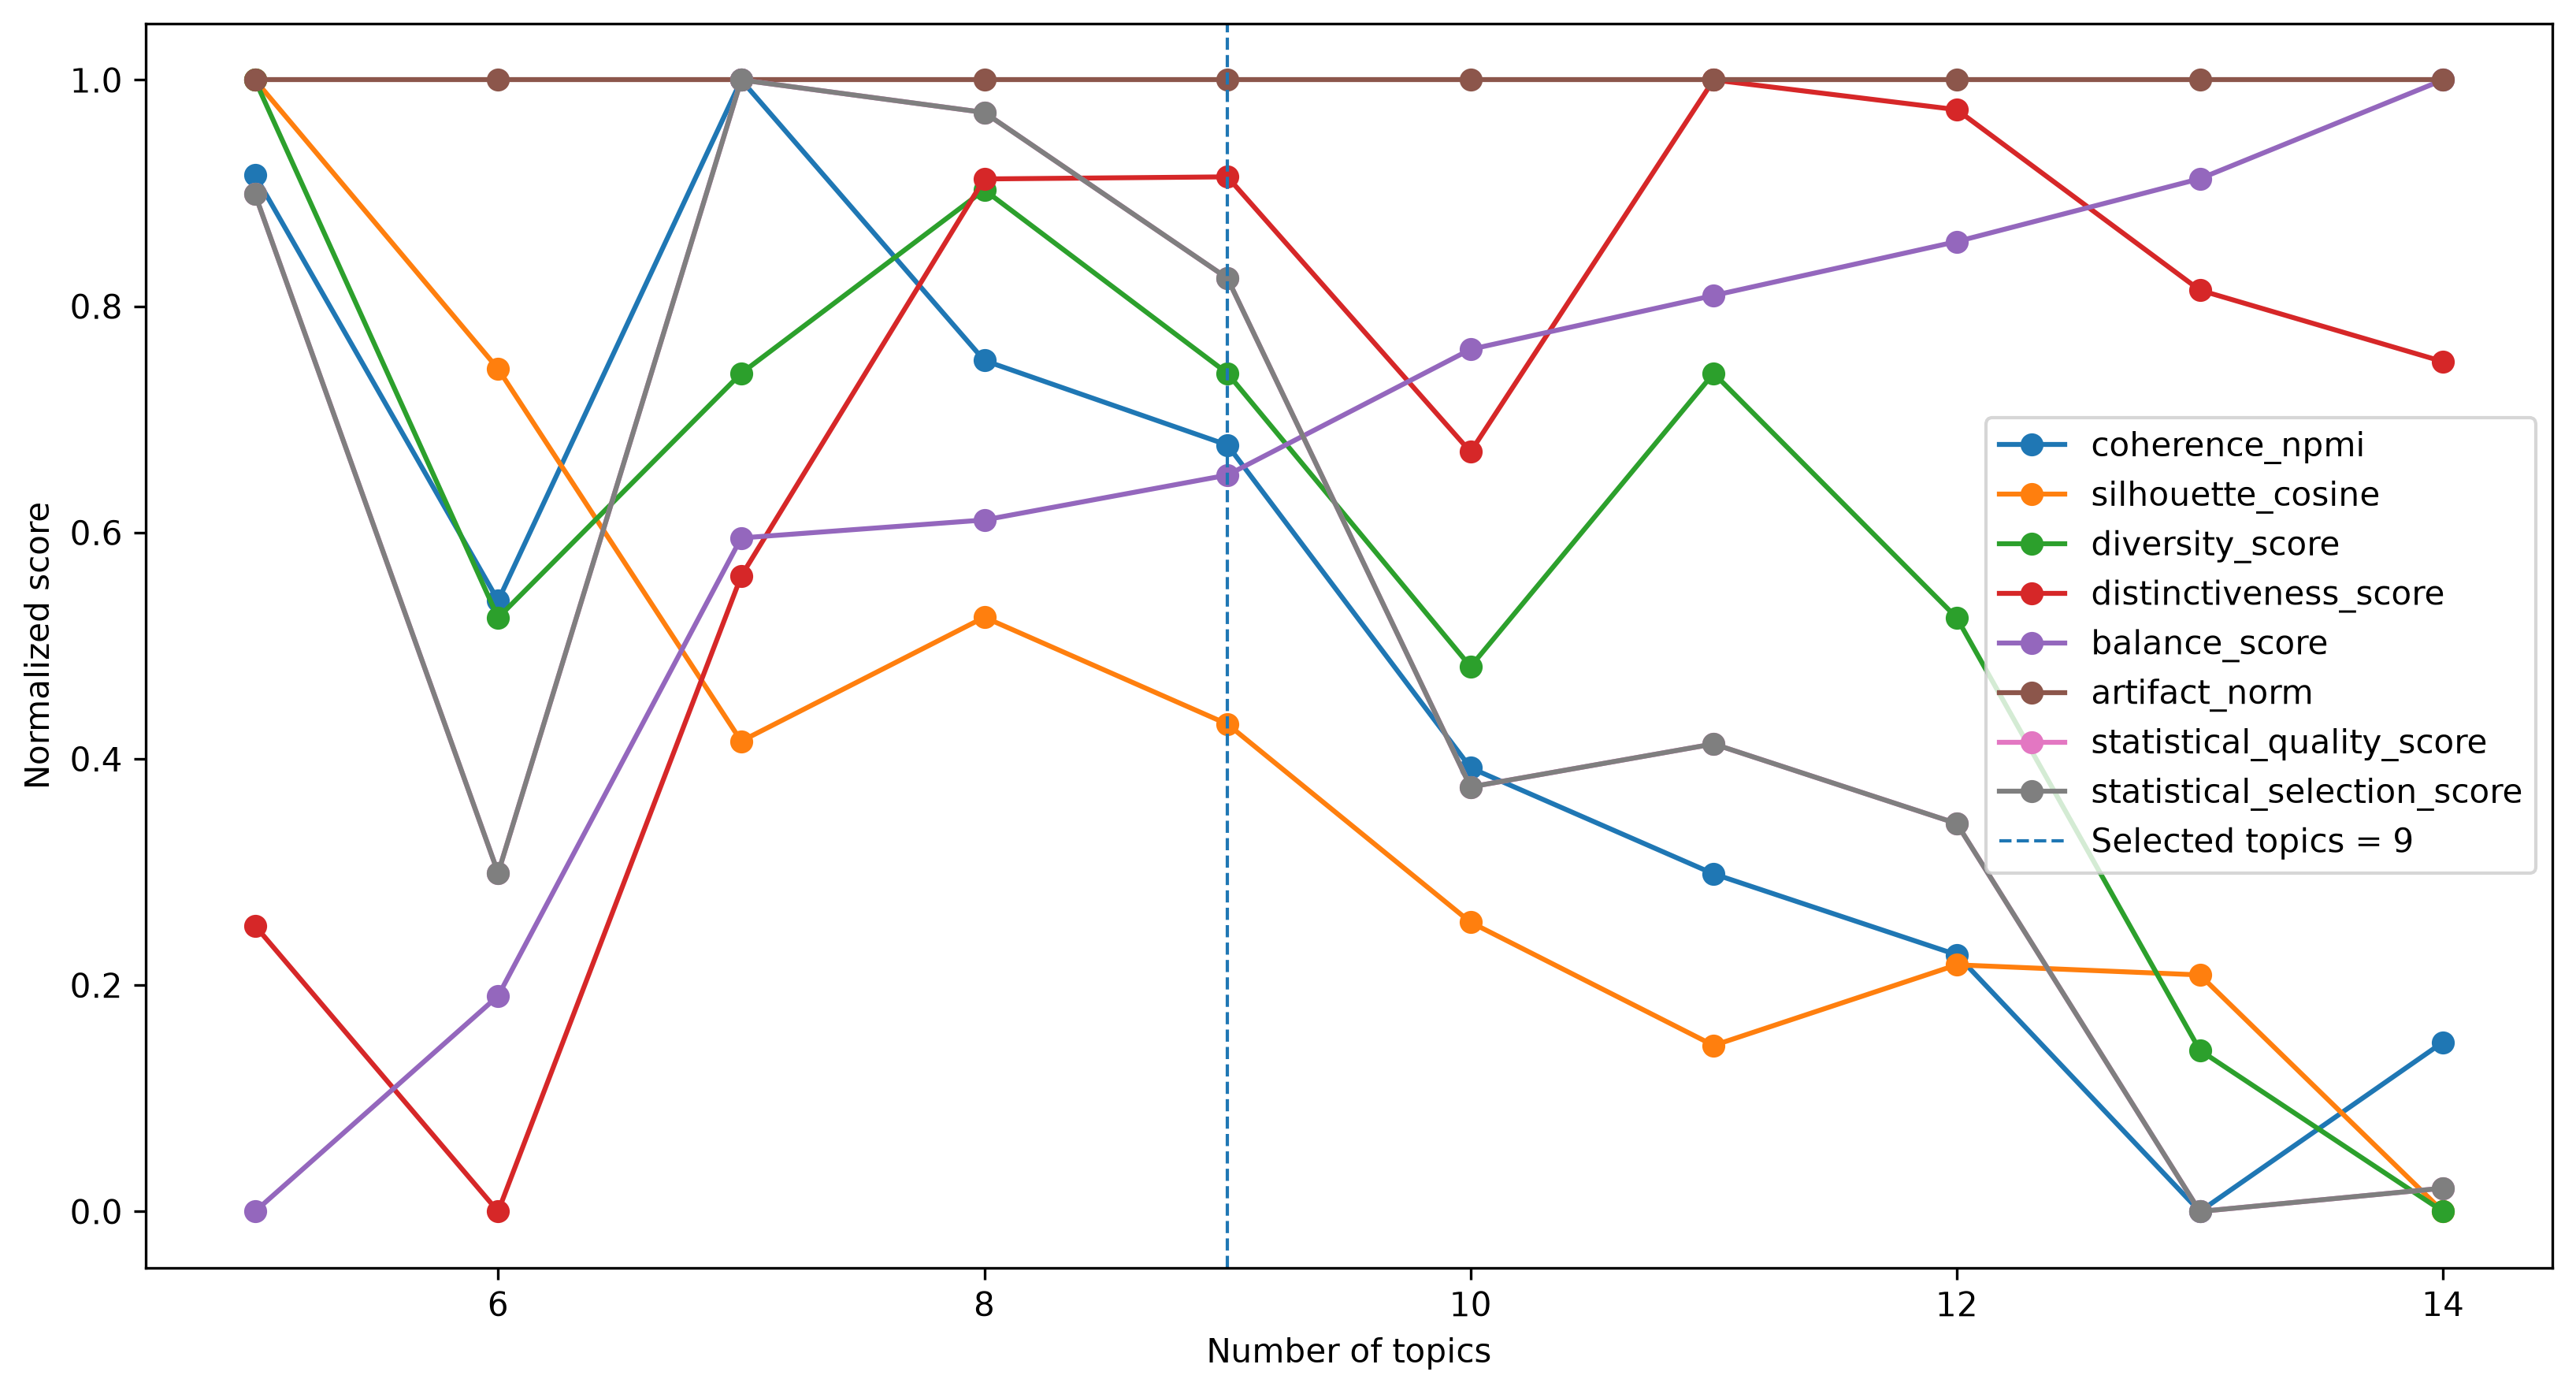
\includegraphics[scale=.26]
    {sentiment_nmf_topic_selection_metrics.png}
    \caption{Topic-number diagnostics.}
\end{subfigure}

\vspace{0.8em}

\begin{subfigure}[t]{0.49\linewidth}
    \centering
    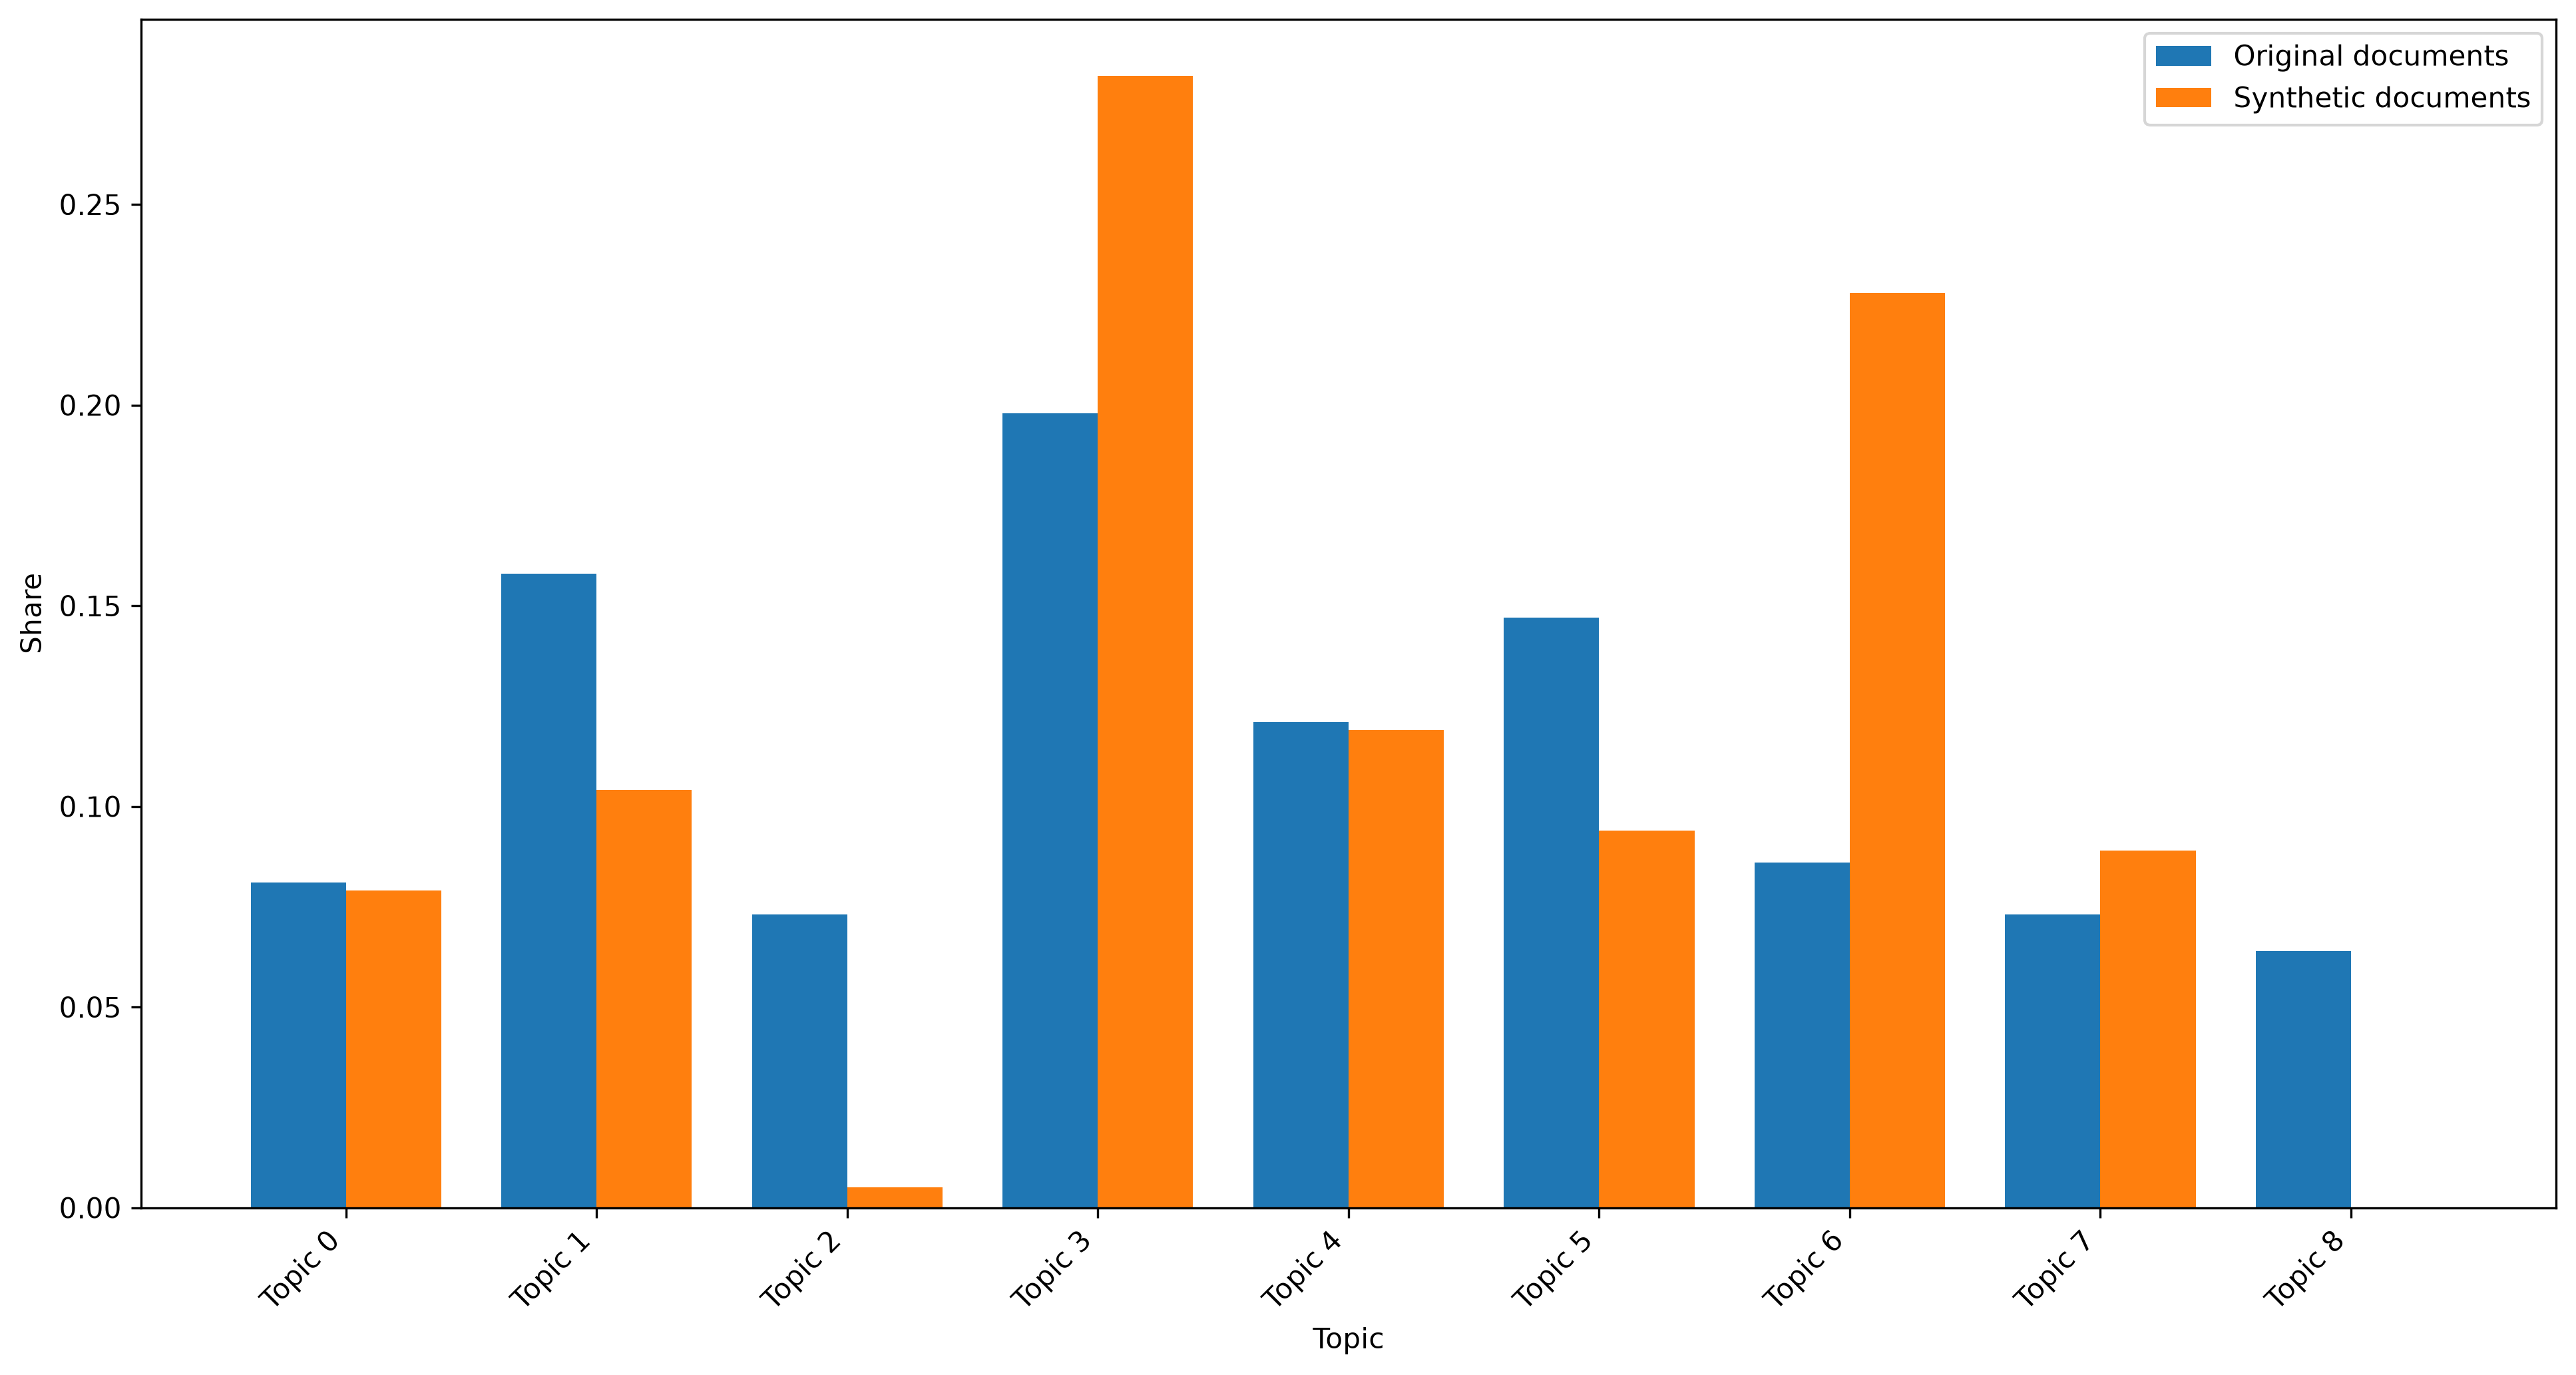
\includegraphics[scale=.21]
    {sentiment_nmf_original_vs_synthetic_distribution.png}
    \caption{Original and synthetic topic shares.}
\end{subfigure}
\hfill
\begin{subfigure}[t]{0.49\linewidth}
    \centering
    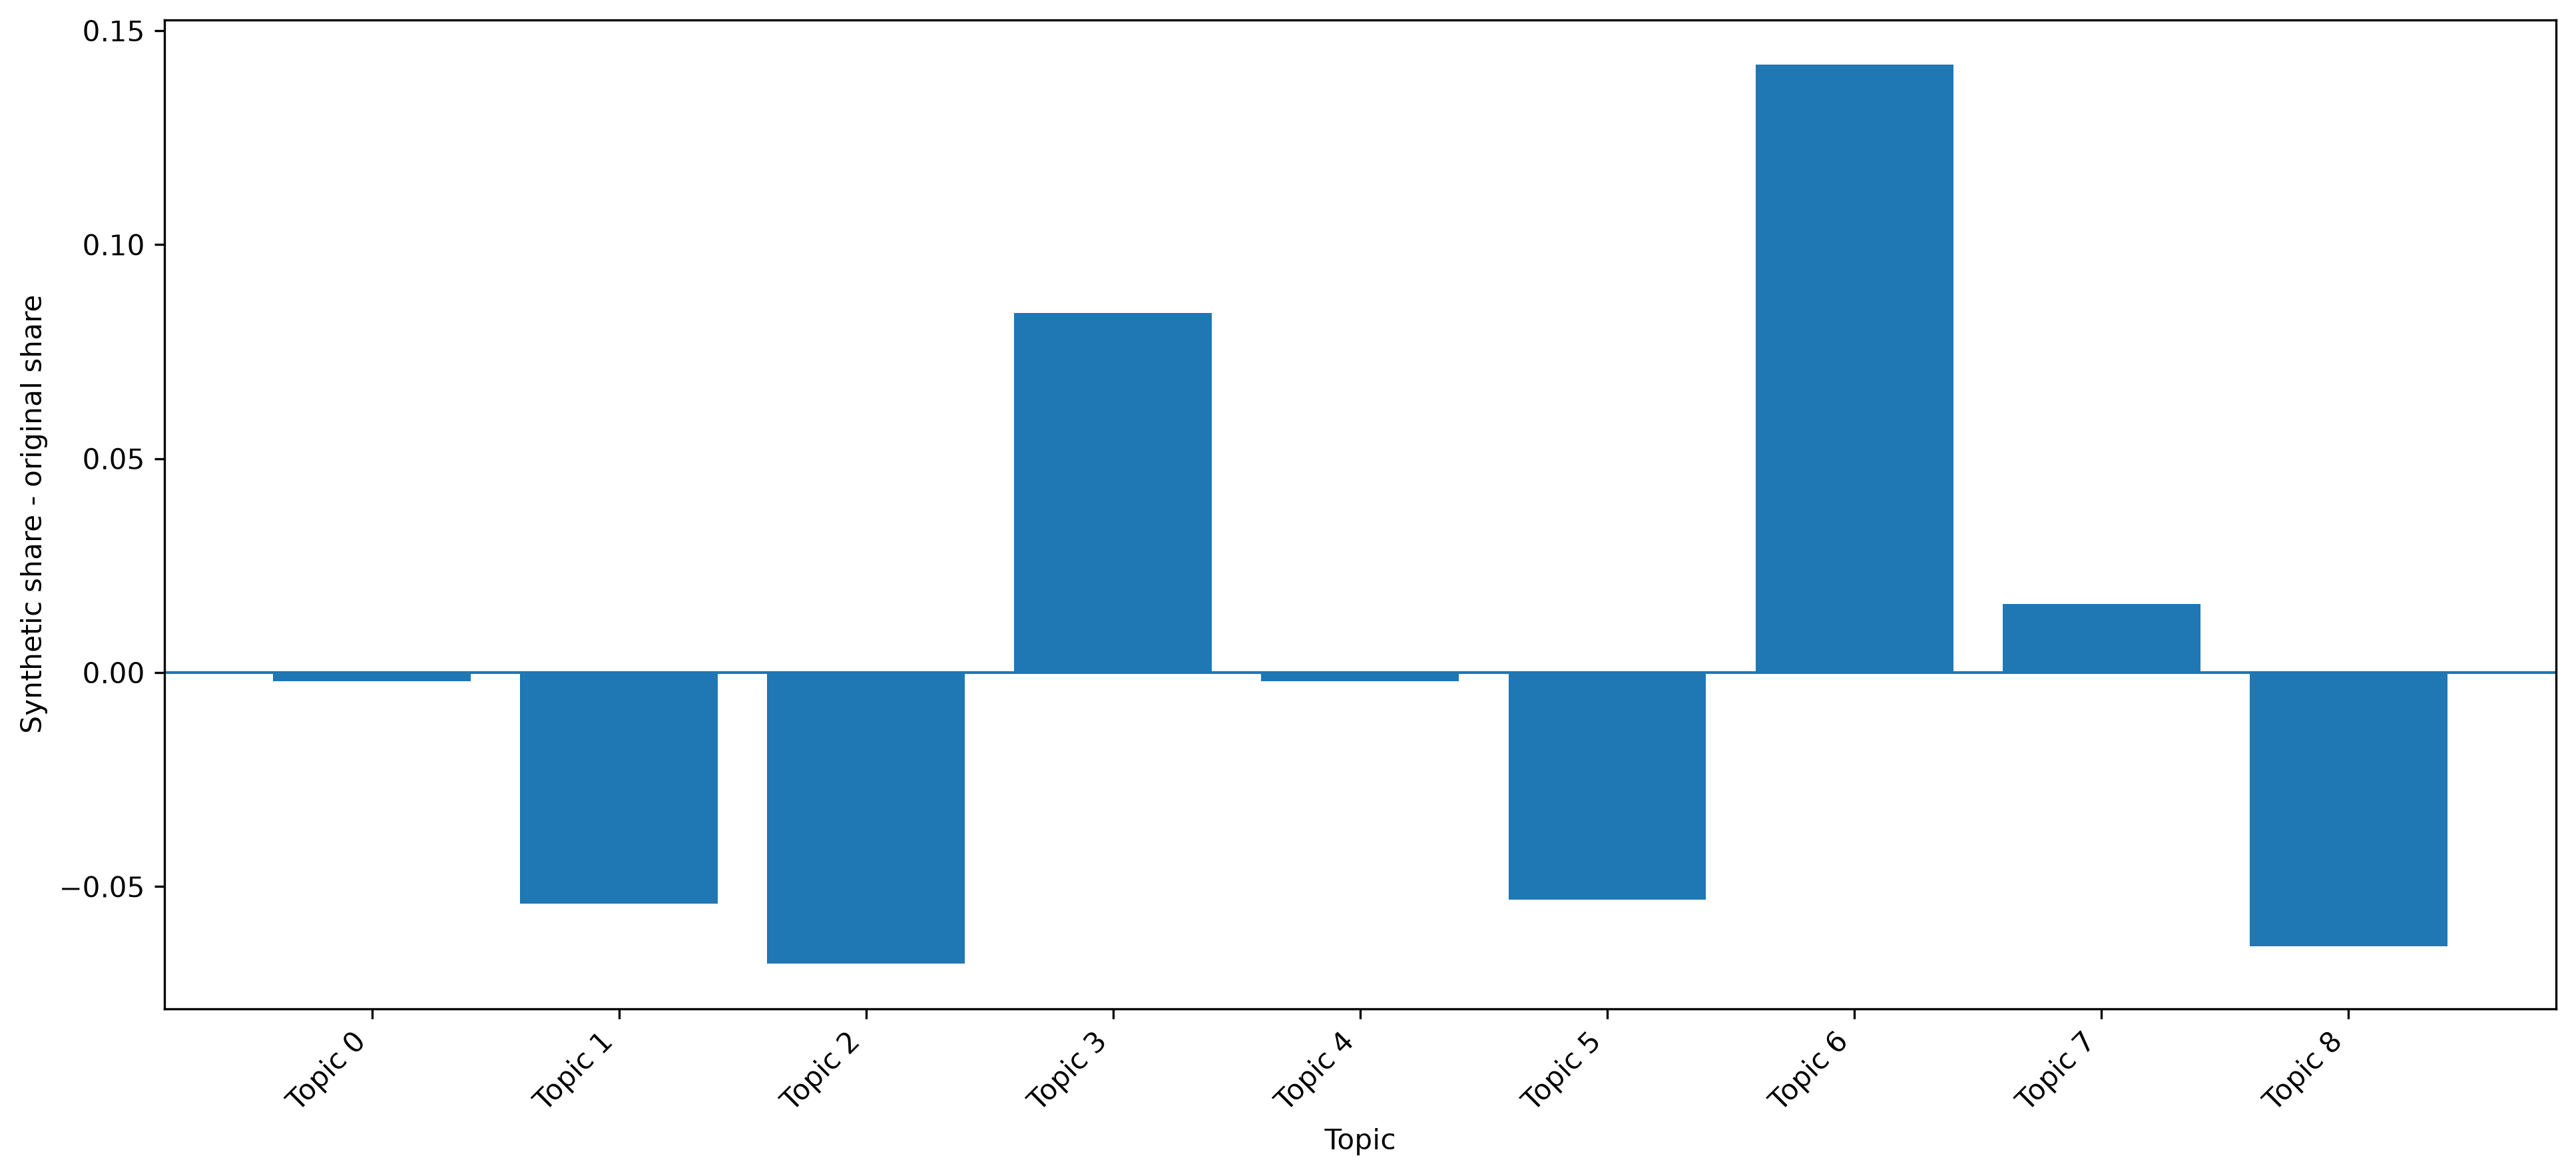
\includegraphics[scale=.22]
    {sentiment_nmf_synthetic_share_difference.png}
    \caption{Synthetic minus original share.}
\end{subfigure}

\caption{Sentiment NMF topic selection and synthetic-sentiment robustness results.}
\label{fig:impl-nmf-sentiment}
\end{figure}

\begin{table}[!htbp]
\centering
\scriptsize
\begin{tabular}{
>{\centering\arraybackslash}p{0.06\linewidth}
>{\raggedright\arraybackslash}p{0.45\linewidth}
rrr
}
\hline
Topic & Short label & Original & Synthetic & Difference \\
\hline
0 & Young people and well-being & 8.1\% & 7.9\% & $-0.2$ pp \\
1 & Student engagement and teacher adaptation & 15.8\% & 10.4\% & $-5.4$ pp \\
2 & GenAI assessment confusion & 7.3\% & 0.5\% & $-6.8$ pp \\
3 & Educator training and ethics & 19.8\% & 28.2\% & $+8.4$ pp \\
4 & Youth-worker perspectives & 12.1\% & 11.9\% & $-0.2$ pp \\
5 & Teacher experience and knowledge & 14.7\% & 9.4\% & $-5.3$ pp \\
6 & Public perception and employment & 8.6\% & 22.8\% & $+14.2$ pp \\
7 & Online-learning intention clarity & 7.3\% & 8.9\% & $+1.6$ pp \\
8 & French digital-technology views & 6.4\% & 0.0\% & $-6.4$ pp \\
\hline
\end{tabular}
\caption{Original and synthetic sentiment shares in the fitted NMF space.}
\label{tab:impl-nmf-synthetic-topics}
\end{table}



The synthetic corpus reproduced Topics~0 and~4 closely, with differences of only
$-0.2$ percentage points. It overrepresented educator training and ethics and public
perceptions of employment, while underrepresenting teacher adaptation, assessment
confusion, teacher experience, and French digital-technology views. Overall, the
synthetic data covered most topics across the retained space but did not preserve
their original proportions uniformly.

\subsection{Comparative Model Selection and Summary}

The three methods were treated as complementary rather than as directly comparable
optimisation problems. LDA supplied a broad probabilistic lexical baseline;
BERTopic-style clustering provided complete and reproducible hard assignments; and
NMF supplied an additive factorisation with explicit document--topic and topic--term
matrices. Their internal selection scores were used to compare candidate solutions
within each method, not to rank unlike modelling spaces.

Table~\ref{tab:impl-workflow-iterations} records the principal pipeline revisions and
the observations that led from one implementation step to the next. Table~\ref{tab:impl-topic-counts} summarises the candidate comparisons and retained
topic counts.

\begin{table}[!htbp]
\centering
\footnotesize
\renewcommand{\arraystretch}{1.0}
\setlength{\tabcolsep}{3pt}
\begin{tabular}{
>{\raggedright\arraybackslash}p{0.24\linewidth}
>{\raggedright\arraybackslash}p{0.32\linewidth}
>{\raggedright\arraybackslash}p{0.38\linewidth}
}
\hline
Initial approach or issue & Observed output & Implemented correction \\
\hline
Automatic acceptance of the highest-ranked topic count & Neighbouring solutions
sometimes contained both fragmented or overlapping topics. & Compare nearby candidates and review their topic outputs before retaining a count. \\[2pt]
Policy BERTopic with nine topics & Several education-practice topics contained
closely related terms, and diversity was absent from the original score. & Add topic
diversity, compare eight and nine, and retain eight. \\[1pt]
Sentiment BERTopic candidate search & Eight topics combined professional-learning
and French public-attitude material. & Compare eight, nine, and ten, and retain nine topics. \\
Synthetic data considered during topic discovery & Synthetic text changed topic
prevalence and, under LDA, produced a separate topic structure. & Keep synthetic data
separate and use it only after empirical fitting or in a separate LDA model. \\[1pt]
Country analysis limited to selected counts & Topic counts alone did not record the
country-specific outputs. & Export global country distributions and separate
country-topic summaries. \\[1pt]
Generic SLM topic phrases & Some initial phrases omitted the population, country, or
policy context visible in the source material. & Use the SLM only after fitting and
manually review the report labels without changing assignments. \\[1pt]
Sentiment NMF automatic plateau choice & Seven had the highest raw score, while nine
produced additional reported topics. & Record the raw winner and the retained
nine-topic output separately. \\[1pt]
Pipeline diagnostics & Artefact or non-converged components could remain unnoticed.
& Retain artefact screening and export reconstruction error, iteration counts, and
convergence diagnostics. \\
\hline
\end{tabular}
\caption{Topic-modelling workflow revisions and implemented corrections.}
\label{tab:impl-workflow-iterations}
\end{table}



\begin{table}[!htbp]
\centering
\small
\begin{tabular}{>{\raggedright\arraybackslash}p{0.20\linewidth}>{\raggedright\arraybackslash}p{0.22\linewidth}>{\raggedright\arraybackslash}p{0.12\linewidth}>{\raggedright\arraybackslash}p{0.34\linewidth}}
\hline
Model & Candidate comparison & Retained topics & Reported observation \\
\hline
Policy LDA & Coherence and diversity search & 4 & Highest retained LDA
combination reported by the search. \\
Original sentiment LDA & Coherence and diversity search & 3 & Original sentiment
retained three topics; synthetic sentiment retained four separately. \\
Policy BERTopic & 8 versus 9 & 8 & Eight had the higher combined score, coherence,
and diversity. \\
Original sentiment BERTopic & 8, 9, and 10 & 9 & Nine had the highest combined
score and coherence. \\
Policy NMF & 8, 9, and 10 & 9 & Nine had the highest combined score and balance,
with equal diversity to eight. \\
Original sentiment NMF & Raw best 7; candidate range 5, 7, 8, 9 & 9 & Seven had the
highest raw score; nine was retained after review of the candidate outputs. \\
\hline
\end{tabular}
\caption{Candidate comparisons and retained topic counts.}
\label{tab:impl-topic-counts}
\end{table}

Equation~\ref{eq:method-synthetic-robustness} was applied to the original and
synthetic share vectors within each retained nine-topic space. The absolute
topic-share differences underlying the total variation distance were averaged and
expressed in percentage points, giving 5.4 for NMF and 8.4 for BERTopic. Synthetic
chunks also covered eight NMF topics, compared with seven BERTopic topics.

These results supported retaining NMF as the reference topic space for the causal NLP
pipelines. The choice reflected operational requirements rather than superiority on
every metric. NMF preserved non-negative topic weights within each chunk, supporting
chunks containing related themes. It also provided fixed topic identifiers, direct
projection through the fitted TF--IDF and factorisation models, and explicit matrices
linkable to causal claims and frames.

\section{Causal NLP Implementation and Results}
\label{sec:impl-causal-nlp}

Following Section~\ref{sec:method-causal-nlp}, two independent causal NLP pipelines
were implemented on the shared cleaned sentence inventory. This section reports their
implemented settings, extracted analytical units, semantic-coverage outputs,
causal-frame network outputs, and synthetic sensitivity checks. The broader assessment
of these results and their cross-method implications is reserved for
Chapter~\ref{chap:analysis}.

\subsection{Shared Sentence Inventory and Extraction Scale}
\label{subsec:impl-causal-inventory}

As defined in Subsection~\ref{subsec:method-shared-causal-cleaning}, both pipelines
imported the cleaning module and verified the sentence-inventory
hash. The filter retained units containing 6--110 words.
{\color{blue} A causal claim linked plausible cause/effect spans through one of six relation families: \texttt{causes\_or\_increases}, \texttt{reduces\_or\_prevents},
\texttt{enables\_or\_supports}, \texttt{requires\_or\_depends\_on},
\texttt{risks\_or\_threatens}, and \texttt{expected\_to\_improve}}. The semantic workflow retained one claim per eligible
sentence; the frame workflow extracted relation occurrences and removed
within-document duplicates. Tables~\ref{tab:impl-causal-scale} and~\ref{tab:impl-causal-settings}
report the resulting analytical units and principal implementation settings.

\begin{table}[!htbp]
\centering
\small
\setlength{\tabcolsep}{5pt}
\begin{tabular}{lrrr}
\hline
Analytical unit & Policy & Original sentiment & Synthetic sentiment \\
\hline
Clean sentences & 15,281 & 4,182 & 2,128 \\
Semantic causal claims & 3,930 & 761 & 761 \\
Validated causal frames & 3,196 & 655 & 674 \\
\hline
\end{tabular}
\caption{Shared causal sentence inventory and method-specific extraction scale.}
\label{tab:impl-causal-scale}
\end{table}

\begin{table}[!htbp]
\vspace*{-.25cm}
    \centering
\scriptsize
\setlength{\tabcolsep}{3.5pt}
\renewcommand{\arraystretch}{1.06}
\begin{tabular}{
>{\raggedright\arraybackslash}p{0.20\linewidth}
>{\raggedright\arraybackslash}p{0.32\linewidth}
>{\raggedright\arraybackslash}p{0.37\linewidth}
}
\hline
Component & Implemented setting & Purpose \\
\hline
Semantic representation &
\texttt{paraphrase-multilingual-MiniLM-L12-v2} &
Provides multilingual sentence embeddings for English and French causal claims. \\

Semantic neighbourhood &
Three nearest claims ($k=3$) &
Uses several candidate matches while retaining a local coverage measure. \\

Balanced comparison &
50 resamples of 761 claims per direction &
Controls the difference between policy and sentiment claim-pool sizes. \\

Inspection threshold &
$\tau=0.511861$, pooled original-sentiment tenth percentile &
Selects claims for manual inspection without defining a validated classification
boundary. \\

Frame acceptance &
Minimum quality score of $0.40$ &
Removes incomplete or weakly formed frames while retaining usable relations. \\

Span-topic projection &
Minimum similarity $0.02$ and minimum margin $0.003$ &
Requires evidence for assigning cause and effect spans to the frozen policy NMF
space. \\

Projection fallback &
Source-document topic for uncertain spans &
Retains valid relations whose short spans cannot be assigned directly. \\

Network sensitivity &
Four specifications and 250 source resamples &
Measures variation under weighting, source composition, frame quality, and projection
rules. \\
\hline
\end{tabular}
\caption{Implemented settings for the semantic-coverage and causal-frame pipelines.}
\label{tab:impl-causal-settings}
\end{table}

All claims and frames retained source-sentence identifiers, preserving
traceability to the cleaned corpus. The frame workflow retained all six relation
families and removed publication residue and repeated within-document relations.
Accepted frames met the quality score of $0.40$. {\color{blue}Span-topic projection
required similarity of at least $0.02$ and a $0.003$ margin over the next-best
topic, limiting weak or ambiguous assignments.} Uncertain projections used the
source-document topic fallback defined in
Subsection~\ref{subsec:method-frame-network}. Projection status, similarity, margin,
and fallback use were retained for inspection.

\subsection{Semantic Causal-Claim Coverage Results}
\label{subsec:impl-semantic-coverage}

The semantic workflow followed Subsection~\ref{subsec:method-semantic-coverage} (see
\texttt{CN1} in Table~\ref{tab:impl-repository-links}). Each claim was compared with
its three nearest claims in the opposite corpus (\(k=3\)), and coverage and deficit
were calculated using Equation~\ref{eq:method-semantic-coverage}. Using three
neighbours provided a balanced local comparison: it reduced dependence on a single
close match without averaging over a broad set of weaker claims. The same value was
applied in both directions to ensure a consistent comparison.

{\small
\begin{verbatim}
Shared cleaned sentence inventory
  -> identify eligible sentences and extract one auditable claim
  -> encode claims with multilingual sentence embeddings
  -> compare each claim with its three nearest opposite-corpus claims
  -> balance both directions through equal-size resampling
  -> calculate directional similarity and coverage deficits
  -> aggregate results globally, by topic, and by country
  -> flag lower-coverage claims using the inspection threshold
  -> project synthetic claims and compare coverage results
\end{verbatim}
}

The directional comparison used 50 equal-size resamples of 761 claims. Following
Equation~\ref{eq:method-balanced-semantic}, policy-to-sentiment mean similarity was
0.6415, producing a mean deficit of 0.3585. Sentiment-to-policy mean similarity was
0.6325, producing a mean deficit of 0.3675. The reverse-direction deficit exceeded
the forward-direction deficit by approximately \(0.0089\).
Table~\ref{tab:impl-semantic-global} reports the balanced outputs.

\begin{table}[!htbp]
\centering
\small
\setlength{\tabcolsep}{5pt}
\begin{tabular}{lrrr}
\hline
Direction & Mean similarity & Mean deficit & 95\% resampling interval \\
\hline
Policy $\rightarrow$ sentiment & 0.6415 & 0.3585 & [0.3534, 0.3638] \\
Sentiment $\rightarrow$ policy & 0.6325 & 0.3675 & [0.3644, 0.3712] \\
\hline
\end{tabular}
\caption{Balanced semantic causal-claim coverage.}
\label{tab:impl-semantic-global}
\end{table}


As reported in Table~\ref{tab:impl-causal-settings}, the inspection threshold was
\(\tau=0.511861\), {\color{blue}the value below which the lowest 10\% of pooled
empirical scores fell.} It selected low-coverage claims for review {\color{blue}and
closer manual inspection}. The audit contained 160 comparisons, but {\color{blue}some
records lacked a completed label stating whether the paired claims matched.}
Threshold counts were therefore used only for inspection, while similarity scores and
deficits remained the pipeline measures. This avoided treating an unchecked cut-off
as evidence of accuracy. {\color{blue}The percentile was a screening rule, not a
validated decision boundary. It flagged relatively weak matches rather than
classifying causal correctness.}

\begin{figure}[ht]
\centering

\begin{subfigure}[t]{0.49\textwidth}
 \centering
 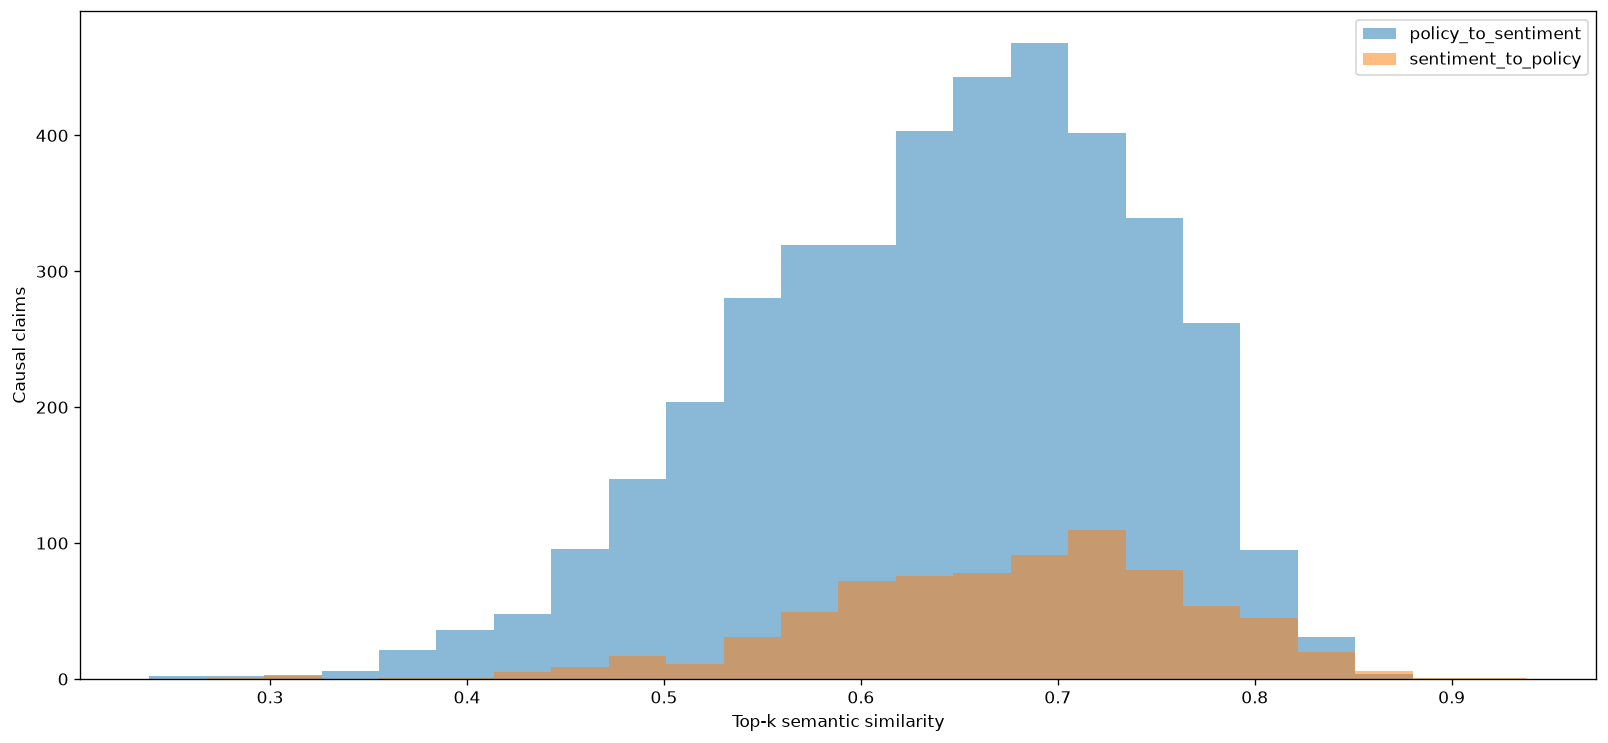
\includegraphics[width=\linewidth]
 {semantic_similarity_histogram.png}
 \caption{Directional top-\(k\) similarity distributions.}
 \label{fig:impl-semantic-distributions}
\end{subfigure}
\hfill
\begin{subfigure}[t]{0.49\textwidth}
 \centering
 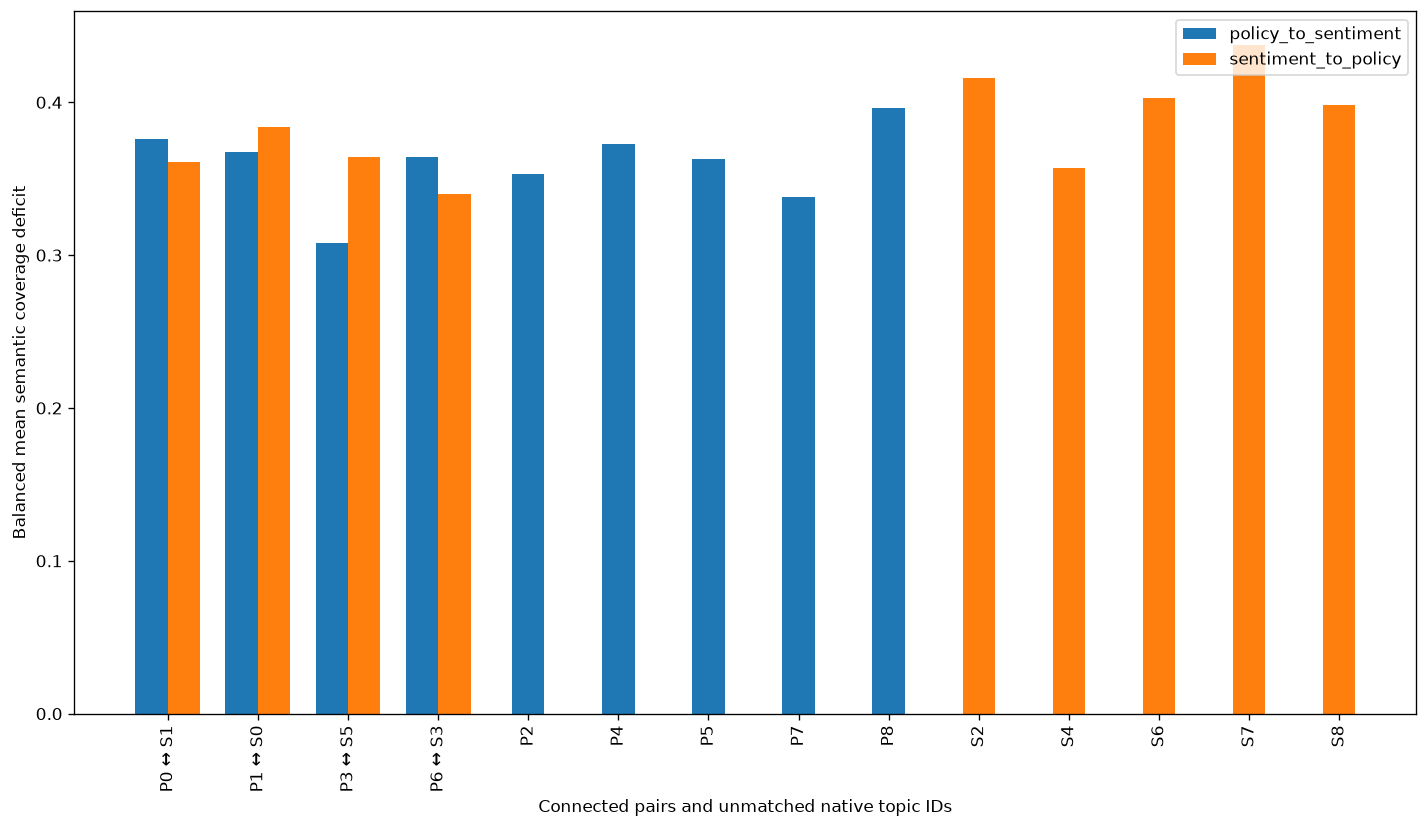
\includegraphics[width=\linewidth]
 {global_semantic_deficit_by_topic_id.png}
 \caption{Balanced native-topic deficits.}
 \label{fig:impl-semantic-topic-deficits}
\end{subfigure}

\vspace{0.8em}

\begin{subfigure}[t]{0.49\textwidth}
 \centering
 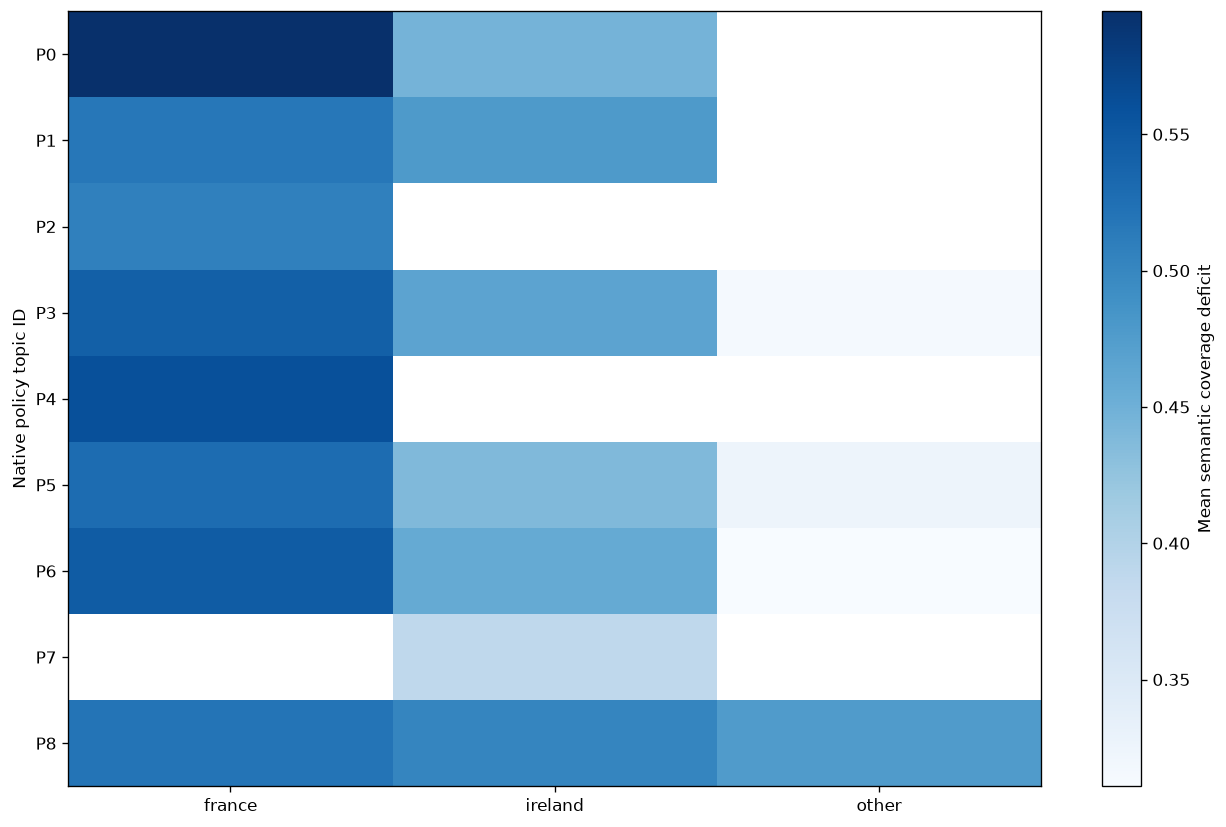
\includegraphics[scale=.15]
 {country_policy_to_sentiment_deficit_by_topic_id.png}
 \caption{Country policy-to-sentiment deficits.}
 \label{fig:impl-semantic-country-forward}
\end{subfigure}
\hfill
\begin{subfigure}[t]{0.49\textwidth}
 \centering
 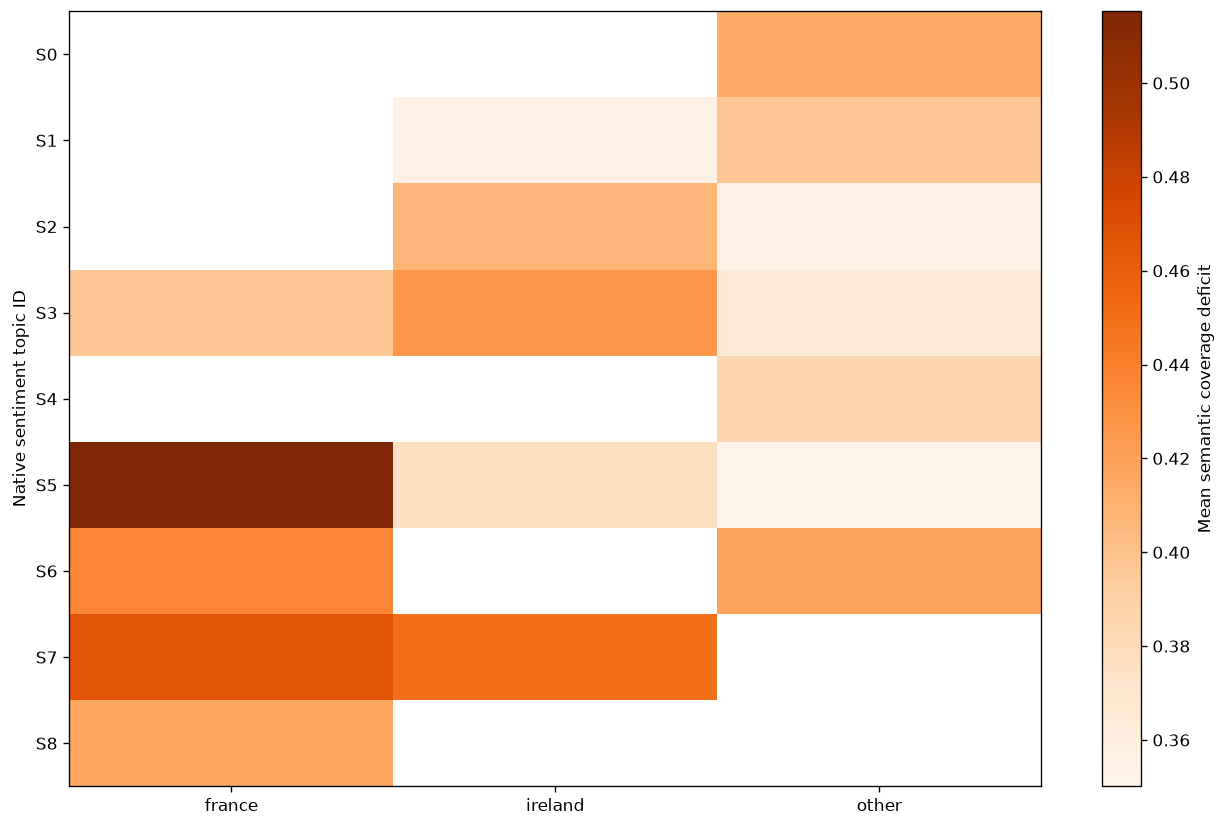
\includegraphics[scale=.15]
 {country_sentiment_to_policy_deficit_by_topic_id.png}
 \caption{Country sentiment-to-policy deficits.}
 \label{fig:impl-semantic-country-reverse}
\end{subfigure}

\caption{Semantic causal-claim coverage results: (a) directional similarity
distributions; (b) global topic deficits; and (c)--(d) country-level directional
deficits. Policy-to-sentiment is shown in blue and sentiment-to-policy in orange in
panel~(a). Empty heatmap cells contain no eligible claims, while darker cells indicate
larger deficits.}
\label{fig:impl-semantic-results}
\end{figure}



As shown in Figure~\ref{fig:impl-semantic-results}(b), P8 (AI curriculum
development and school oversight) had the largest balanced policy-topic deficit at
0.3960, followed by P0 (AI-assisted learning-assessment protocols) at 0.3763, P4
(cognitive offloading in AI-assisted education) at 0.3729, and P1 (AI child
protection and rights) at 0.3677. P8 contained 431 claims from 26 documents, P0
contained 604 claims from 29 documents, and P4 drew on six documents. P3 (AI
competency-framework and curriculum development) had the smallest deficit at
0.3079. The P8 and P0 values had broader document support, whereas P4 reflected a
narrower source base. Among sentiment topics, the largest deficits occurred for S7
(online-learning intention clarity and classroom relevance), S2 (GenAI detection and
assessment confusion), and S6 (public perceptions of AI and youth employment).
These results locate the strongest semantic gaps in curriculum oversight, assessment,
and selected sentiment themes, with differing levels of support.

Synthetic claims were projected into the original semantic analysis only as a
sensitivity check. Following Equation~\ref{eq:method-semantic-synthetic-change},
most native sentiment-topic deficits changed by small amounts, while S2 changed by
approximately \(-0.057\). No synthetic claims were assigned to S8, so no change was
calculated for that topic. Synthetic outputs remained separate from the original
coverage results.

The country-level results are shown in
Figure~\ref{fig:impl-semantic-results}(c)--(d). France had its largest
policy-to-sentiment deficits for P0 and P6, although some cells contained claims
from only one to three documents. Ireland had broader source support, with P8
producing its largest forward deficit and S7 its largest reverse-direction deficit.
Empty cells indicate that no eligible claims were available for the
comparison.

\subsection{Causal-Frame Network Results}
\label{subsec:impl-frame-networks}

The causal-frame workflow followed
Subsection~\ref{subsec:method-frame-network}
(see \texttt{CN2} in Table~\ref{tab:impl-repository-links}). It extracted cause,
relation, and effect spans, calculated frame-quality scores, projected both spans into
the frozen policy NMF space, and constructed weighted policy and sentiment networks.

{\small
\begin{verbatim}
Shared cleaned sentence inventory
  -> detect English and French causal cues
  -> extract cause, relation, and effect spans
  -> validate frames and calculate quality scores
  -> remove repeated relations within each document
  -> project cause and effect spans to frozen policy NMF topics
  -> build weighted policy and sentiment frame networks
  -> calculate global divergence and topic-level gaps
  -> run specification, source-resampling, and synthetic checks
\end{verbatim}
}

Using Equation~\ref{eq:method-frame-js}, the quality-weighted network produced
\(D_{\mathrm{JS}}=0.2596\). The source-balanced, high-quality-frame, and
directly projected-span specifications produced 0.2425, 0.2738, and 0.2964,
respectively. Across 250 source-level resamples, mean divergence was 0.3359, with
a 2.5th--97.5th percentile range of 0.2663--0.4157. This range reflects variation
in source composition rather than a conventional confidence interval.
Table~\ref{tab:impl-frame-robustness} reports the four specifications.
{\color{blue}Divergence remained across specifications, suggesting no single
weighting choice explained the result. The higher projected-only value suggests
that excluding fallback assignments increased network differences.}

\begin{table}[!htbp]
\centering
\small
\setlength{\tabcolsep}{4.5pt}
\begin{tabular}{lccc}
\hline
Specification & Policy frames & Sentiment frames & \(D_{\mathrm{JS}}\) \\
\hline
Quality-weighted primary & 3,196 & 655 & 0.2596 \\
Source-balanced only & 3,196 & 655 & 0.2425 \\
High-quality frames only & 2,513 & 547 & 0.2738 \\
Reliable projected spans only & 1,540 & 294 & 0.2964 \\
\hline
\end{tabular}
\caption{Causal-frame network divergence across four specifications.}
\label{tab:impl-frame-robustness}
\end{table}

\begin{figure}[!htbp]
\centering

\begin{subfigure}[t]{0.32\textwidth}
 \centering
 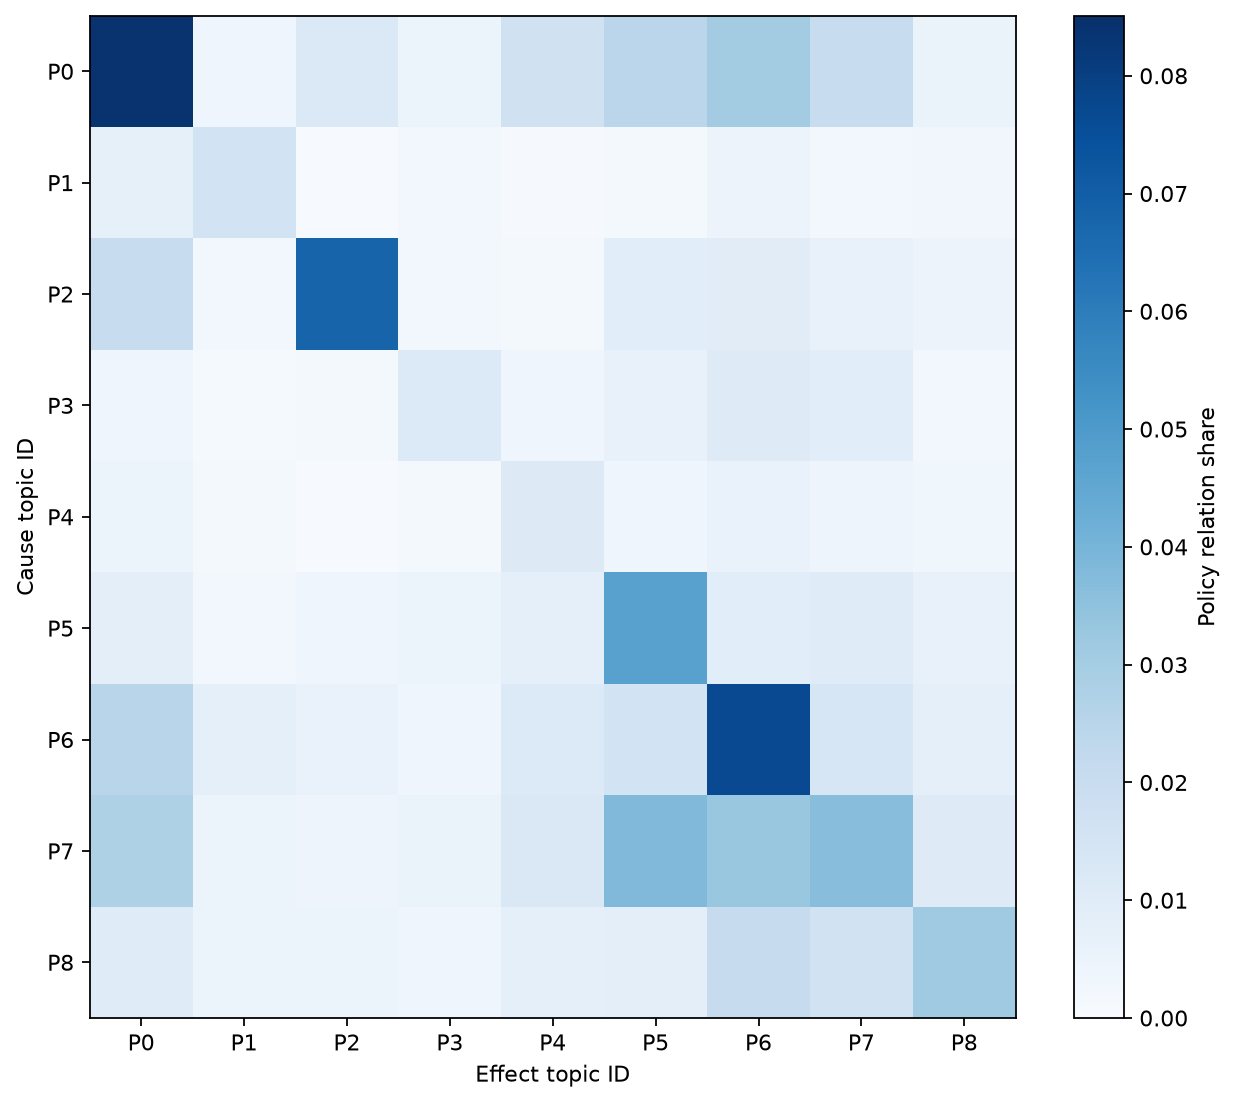
\includegraphics[width=\linewidth]
 {global_policy_causal_frame_matrix.png}
 \caption{Policy matrix.}
 \label{fig:impl-frame-policy-matrix}
\end{subfigure}
\hfill
\begin{subfigure}[t]{0.32\textwidth}
 \centering
 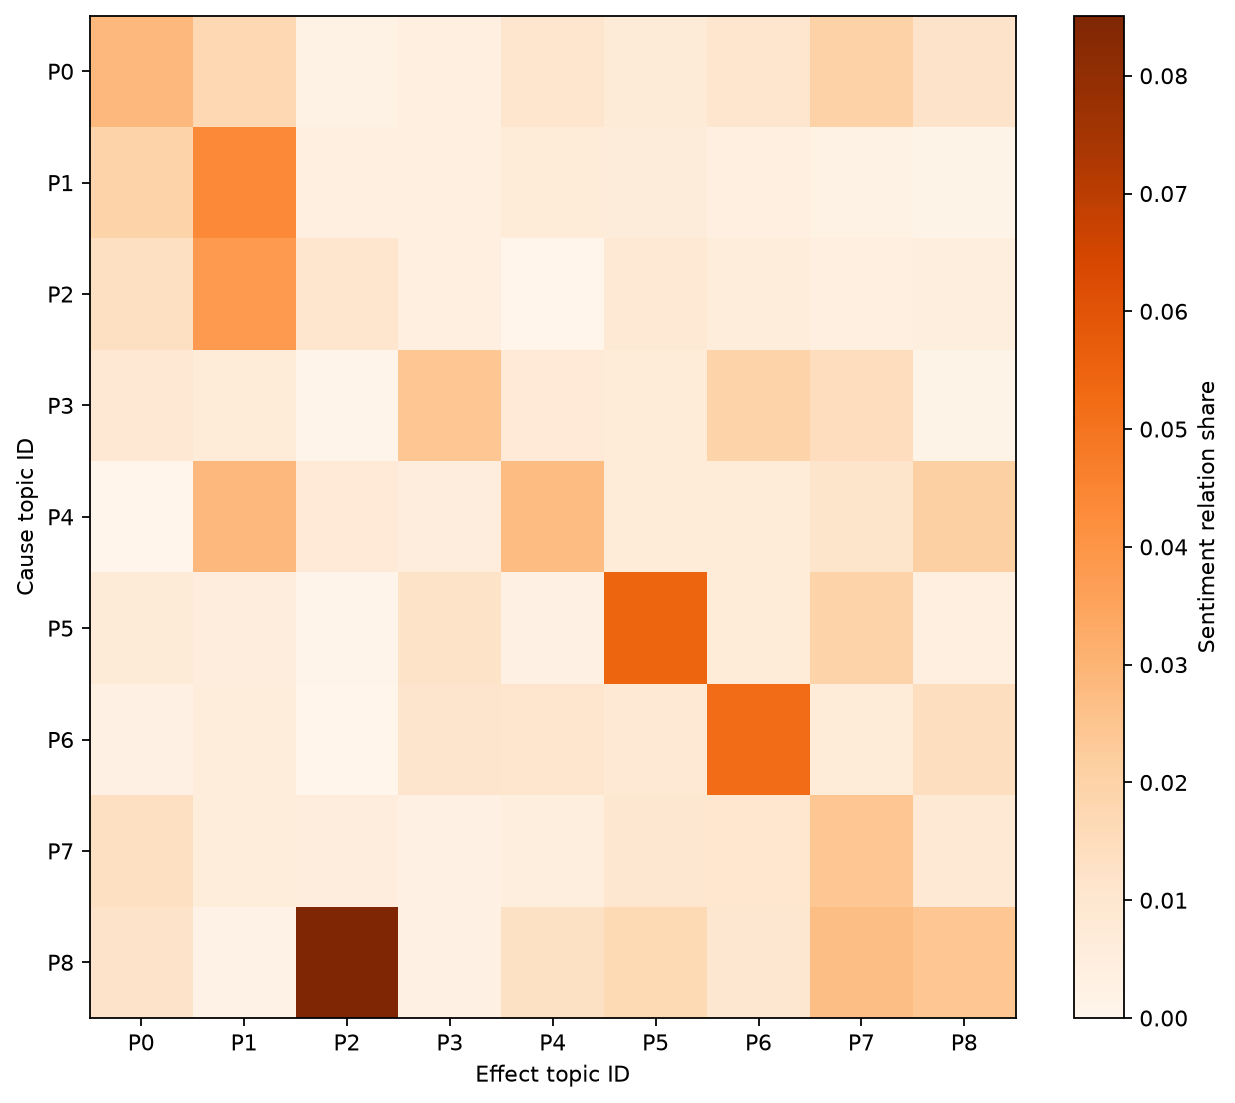
\includegraphics[width=\linewidth]
 {global_sentiment_causal_frame_matrix.png}
 \caption{Sentiment matrix.}
 \label{fig:impl-frame-sentiment-matrix}
\end{subfigure}
\hfill
\begin{subfigure}[t]{0.32\textwidth}
 \centering
 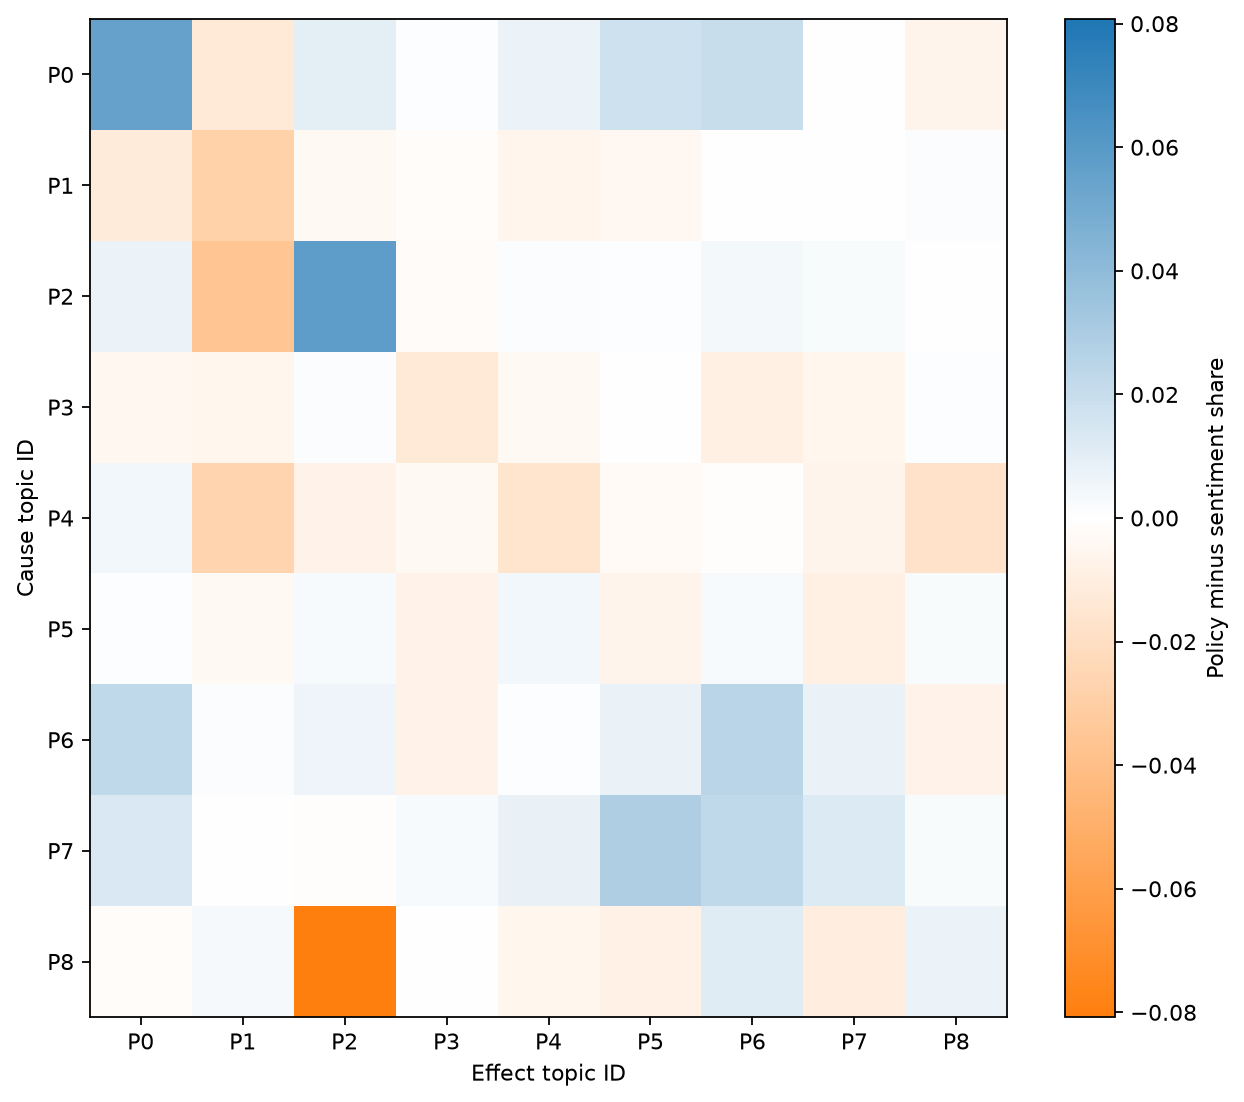
\includegraphics[width=\linewidth]
 {global_causal_frame_gap_matrix.png}
 \caption{Signed share differences.}
 \label{fig:impl-frame-gap-matrix}
\end{subfigure}

\caption{Global causal-frame matrices in the frozen policy NMF topic space.
Panels~(a) and~(b) show policy and sentiment frame shares projected onto the common
\(P0\)--\(P8\) axes. Panel~(c) shows their signed differences, where blue indicates
greater policy weight and orange greater sentiment weight, {\color{blue}highlighting
the strongest contrasts}.}
\label{fig:impl-frame-matrices}
\end{figure}

Document-topic fallback was used for approximately 31--35\% of cause and effect span
assignments, depending on corpus and span role. {\color{blue}Exact zero-similarity
assignments were cases where a span had no measurable similarity to any policy
topic.} They were absent from sentiment and accounted for approximately 0.1\% of
policy assignments. The reliable-projection specification excluded fallback
assignments and retained only spans meeting the similarity and margin rules.

Figure~\ref{fig:impl-frame-matrices}(a)--(b) compares the normalised cause--effect
matrices for policy and original sentiment. Policy placed greater weight on the
P0--P0, P2--P2, and P6--P6 connections, while sentiment showed a stronger P8--P2
connection and greater weight in several cells ending in P1. The signed matrix in
panel~(c) locates these differences directly: positive cells indicate greater policy
weight and negative cells greater sentiment weight. This view complements the global
divergence by identifying the topic pairs contributing to the structural difference.
{\color{blue}In practice, these patterns indicate which topic-to-topic causal links
received relatively greater weight in each corpus. They describe differences in the
extracted frame distributions, rather than establishing stronger real-world causal
relationships between the topics.}



\begin{figure}[ht]
\centering

\begin{subfigure}[t]{0.49\textwidth}
 \centering
 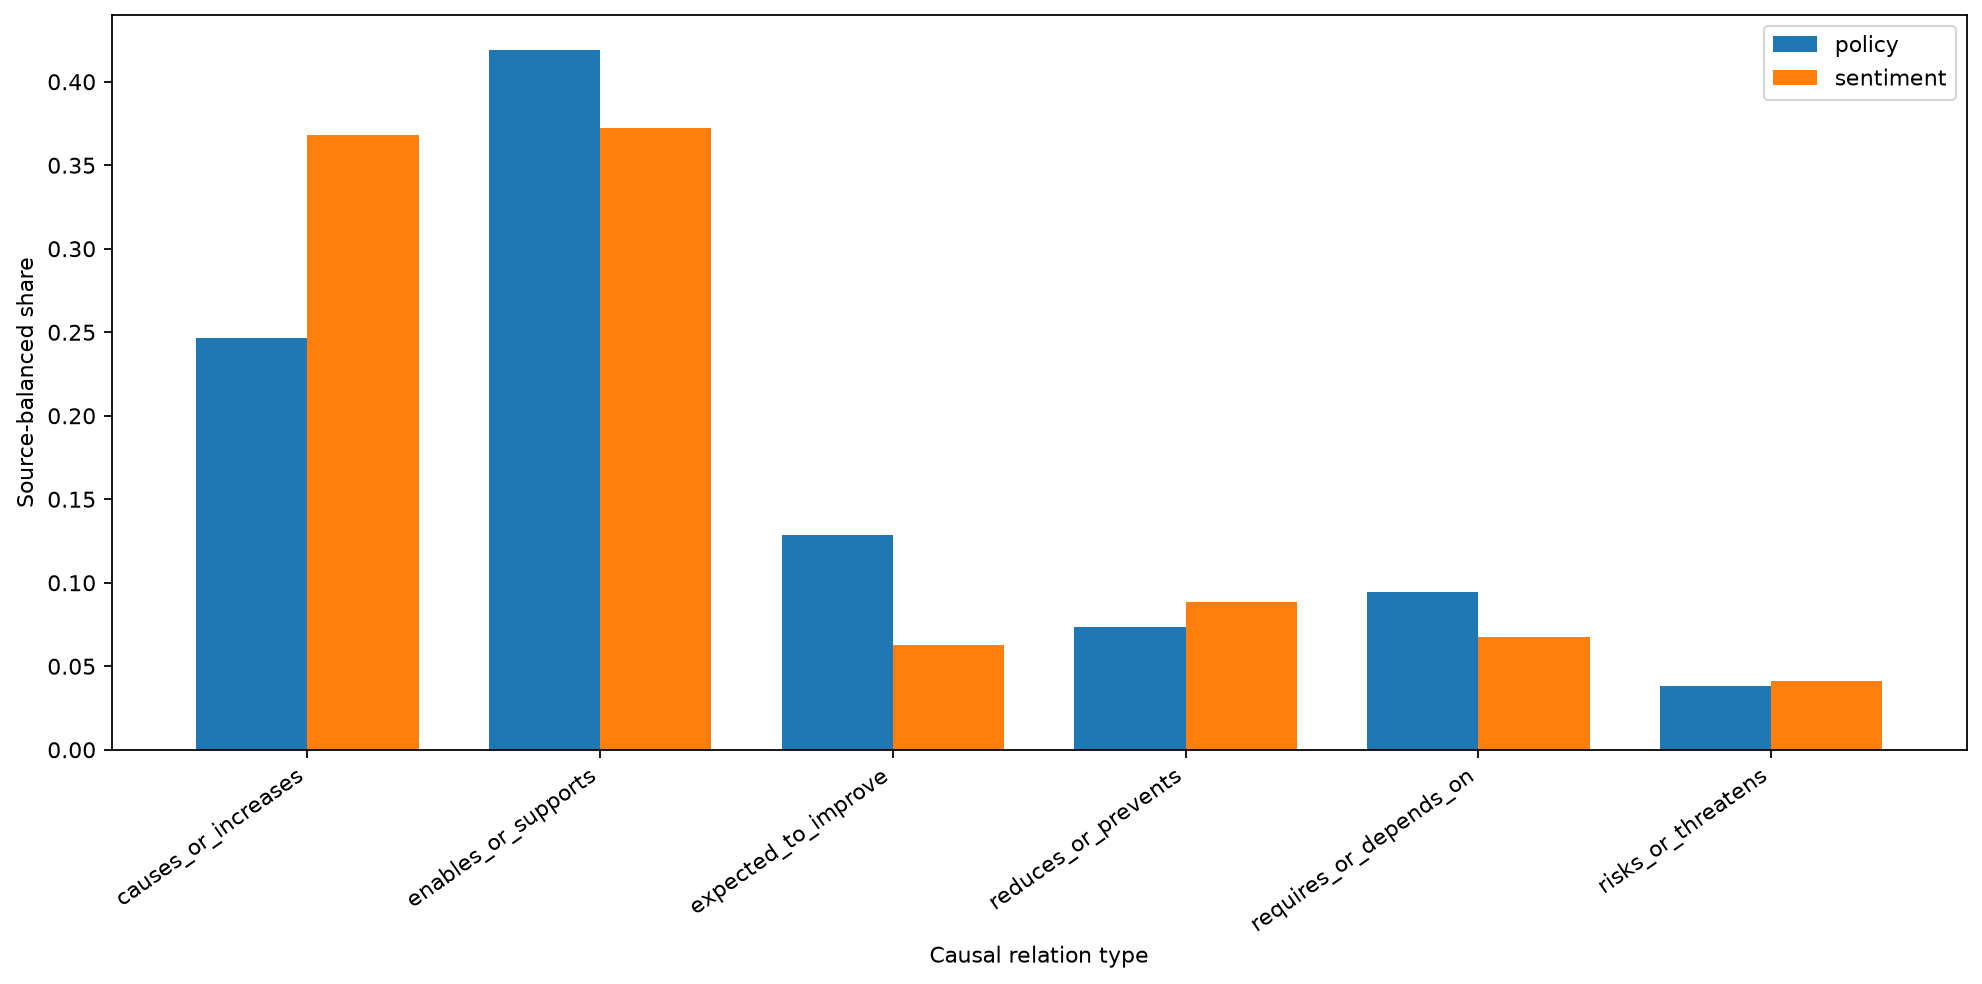
\includegraphics[width=\linewidth]
 {global_causal_frame_relation_types.png}
 \caption{Relation-family shares.}
 \label{fig:impl-frame-relation-shares}
\end{subfigure}
\hfill
\begin{subfigure}[t]{0.49\textwidth}
 \centering
 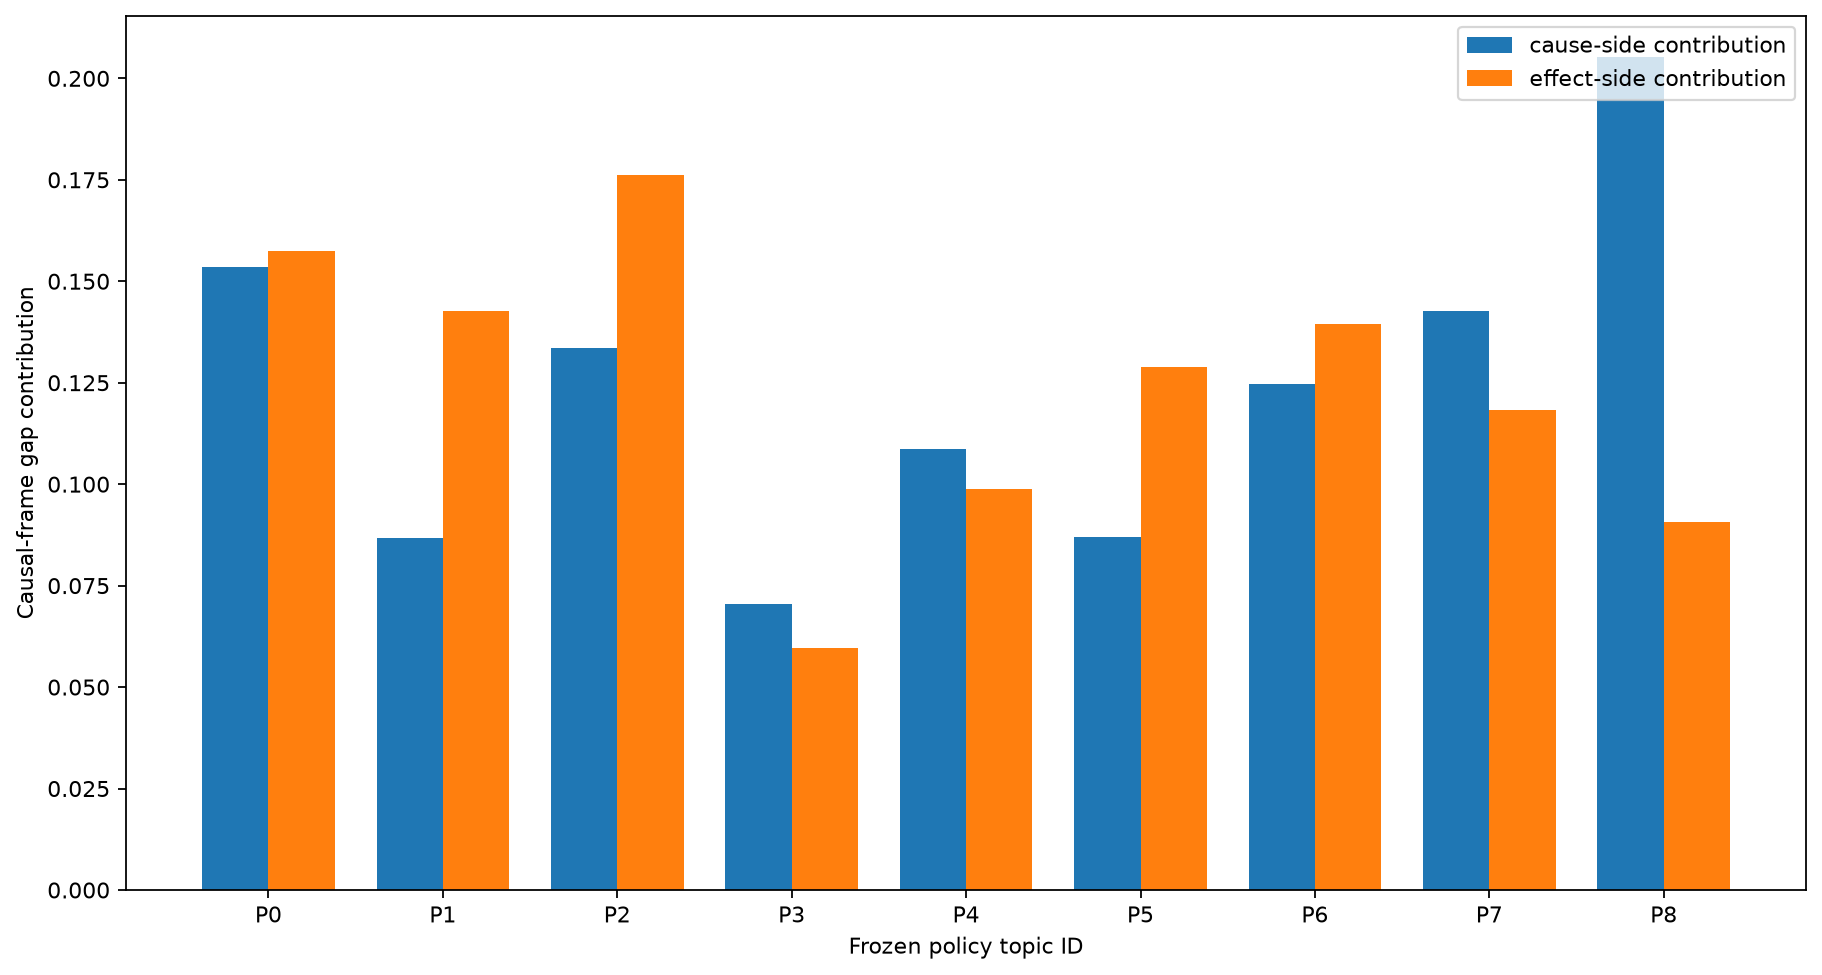
\includegraphics[width=\linewidth]
 {global_causal_frame_gap_by_topic_id.png}
 \caption{Cause- and effect-side topic gaps.}
 \label{fig:impl-frame-topic-gaps}
\end{subfigure}

\vspace{0.8em}

\begin{subfigure}[t]{0.66\textwidth}
 \centering
 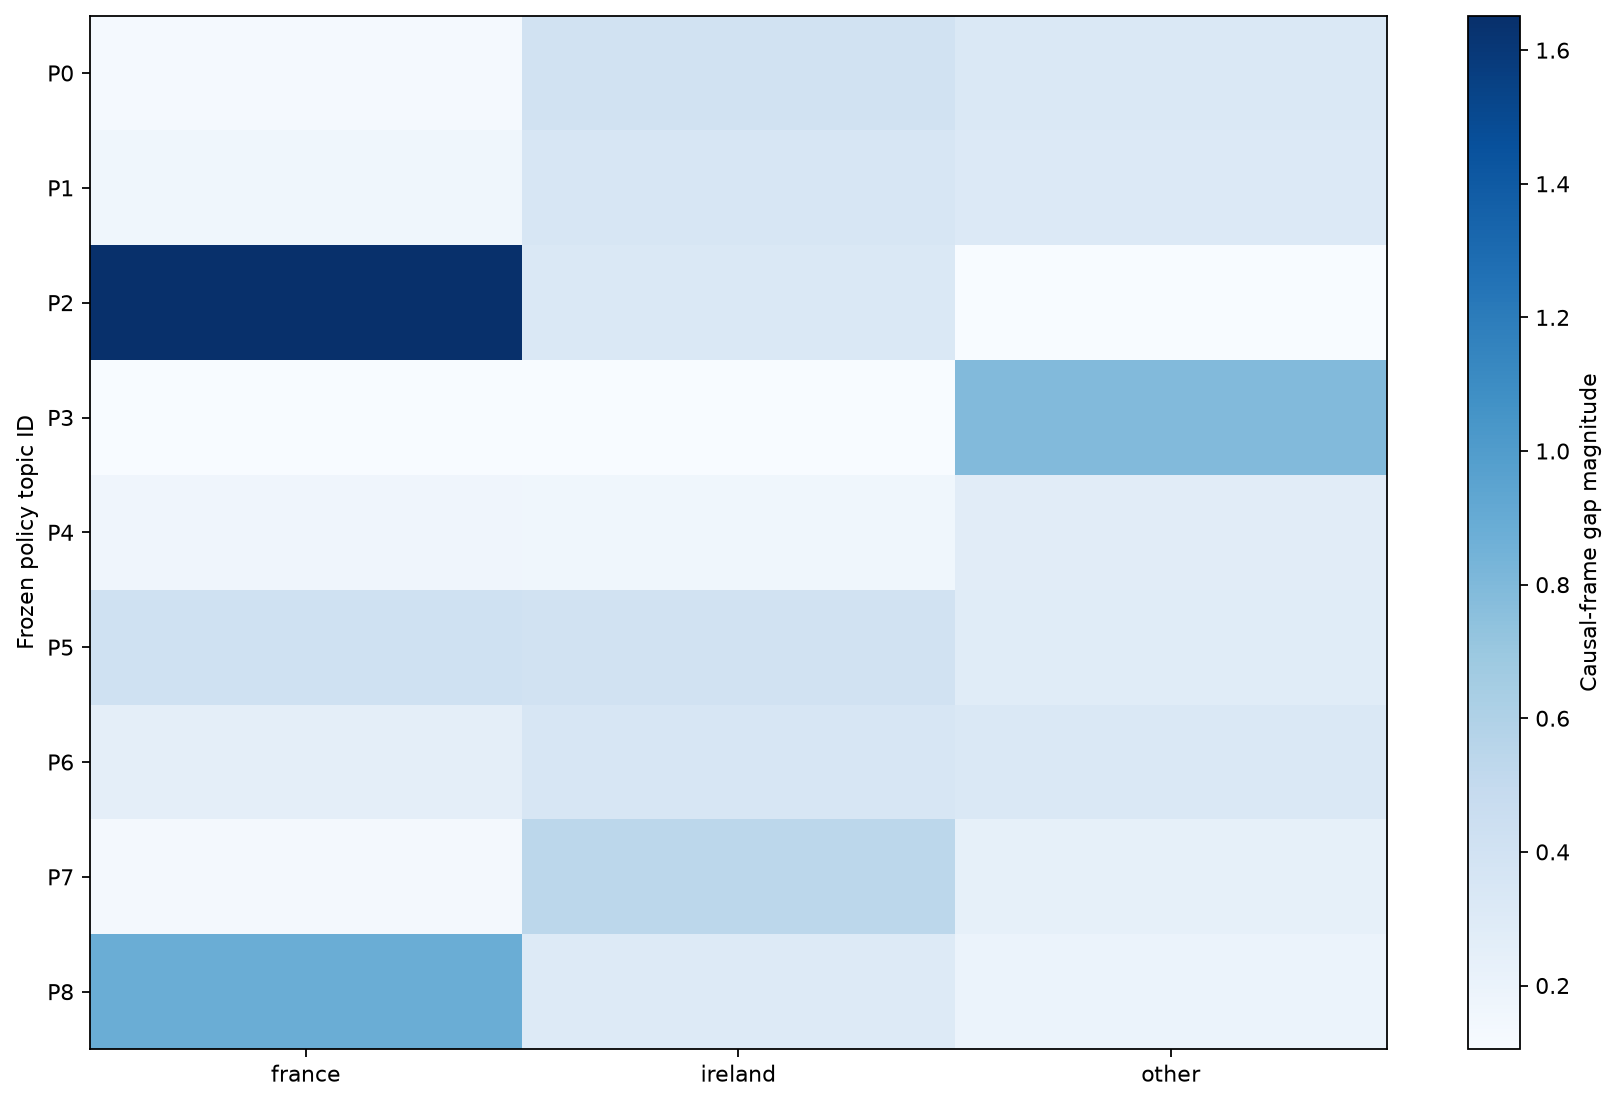
\includegraphics[scale=0.13]
 {country_causal_frame_gap_by_topic_id.png}
 \caption{Country-level frame gaps by policy topic.}
 \label{fig:impl-frame-country}
\vspace*{-.25cm}
\end{subfigure}

\caption{Causal-frame network results: (a) global relation-family shares;
(b) global topic-level gaps; and (c) country-level gap magnitudes. Policy is shown
in blue and sentiment in orange in panel~(a). Darker cells in panel~(c) indicate
larger combined cause- and effect-side gaps.}
\label{fig:impl-frame-results}
\end{figure}


As shown in Figure~\ref{fig:impl-frame-results}(a), relation-family shares differed
most for causes/increases, which accounted for 36.8\% of sentiment frame weight and
24.7\% of policy weight. Policy assigned 41.9\% to enables/supports, compared with
37.2\% in sentiment; 12.9\% to expected improvement, compared with 6.3\%; and 9.4\%
to requirements/dependencies, compared with 6.8\%. Risk/threat relations accounted
for 3.8\% of policy weight and 4.1\% of sentiment weight.
{\color{blue}These shares suggest different emphases in the extracted relation
families rather than differences in causal strength. Representative causal links
underlying these patterns are examined in Chapter~5.}


The synthetic-frame check produced \(D_{\mathrm{JS}}=0.3611\), compared with 0.2596
for the original sentiment network, a difference of approximately 0.1015. The
requirements/dependencies family produced the largest relation-share change under
synthetic input. Synthetic frames remained separate from the original network.
Following Equation~\ref{eq:method-topic-gap}, P0 had the largest topic-level gap at
0.3109, followed by P2 at 0.3099 and P8 at 0.2959. P6 and P7 produced gaps of 0.2641
and 0.2609, while P3 produced the smallest value at 0.1301. These results are shown
in Figure~\ref{fig:impl-frame-results}(b). The leading topic-level outputs drew on
54--60 source documents. {\color{blue}Larger gaps indicate greater differences in
how topics participate in extracted cause--effect links. Specific links contributing
to these differences are discussed in Chapter~5.}

The topic-level measure \(G_t\) is an unnormalised sum of incoming and outgoing
absolute differences. It is non-negative but is not bounded above by one and is
therefore interpreted separately from the global Jensen--Shannon divergence. The
country outputs are shown in Figure~\ref{fig:impl-frame-results}(c) for France,
Ireland, and the pooled Other European group. France had its largest values for P2
and P8, with P2 reaching 1.6518. Ireland had its largest value for P7 at 0.5391,
followed by P0 and P5 at approximately 0.397. The pooled Other European group had its
largest value for P3 at 0.7929. France and Ireland each contained three original
sentiment sources. {\color{blue}These values identify where structural differences
are most evident; their substantive meaning is considered in Chapter~5.}

% The substantive interpretation and assessment of the directional, topic-level,
% country-level, relation-family, source-support, and global network differences are
% presented in Section~\ref{sec:analysis-gap}.

\section{LLM-Assisted Causal-Gap Discovery}
\label{sec:impl-llm-causal-gap}